% !TeX program = xelatex
%% 부득이하게 pdflatex을 사용해야 할 경우 위의 magic comment를 제거하십시오.

%%%%%%%%%%%%%%%%%%%%%%%%%%%%%%%%%%%%%%%%%%%%%%%%%%%%%%%%%%%%%%%%%%%%%%%%%%%%%%%%%
%%%  LaTeX document class of the thesis of the Gyeonggi Science High School   %%%
%%%  Last edition 2015.11.13 by Chinook Mok                                   %%%
%%%  Continously being modified by gshslatexintro after 2016.02.02.           %%%
%%%  Check the latest version at : latex.gs.hs.kr                             %%%
%%%  Also refer to https://www.facebook.com/gshstexsociety                    %%%
%%%%%%%%%%%%%%%%%%%%%%%%%%%%%%%%%%%%%%%%%%%%%%%%%%%%%%%%%%%%%%%%%%%%%%%%%%%%%%%%%

\documentclass{gshs_thesis}

\graphicspath{{images/}}
% 이곳에 필요한 별도의 패키지들을 적어넣으시오.
%\usepackage{...}
\usepackage{verbatim} % for commment, verbatim environment
\usepackage{spverbatim} % automatic linebreak verbatim environment
\usepackage{listings}
\lstset{
	basicstyle=\small\ttfamily,
	columns=flexible,
	breaklines=true
}
\usepackage{hologo}

% -----------------------------------------------------------------------
%                   이 부분은 수정하지 마시오.
% -----------------------------------------------------------------------
\titleheader{졸업논문청구논문}
\school{과학영재학교 경기과학고등학교}
\approval{위 논문은 과학영재학교 경기과학고등학교 졸업논문으로\\
졸업논문심사위원회에서 심사 통과하였음.}
\chairperson{심사위원장}
\examiner{심사위원}
\apprvsign{(인)}
\korabstract{초 록}
\koracknowledgement{감사의 글}
\korresearches{연 구 활 동}

%: ----------------------------------------------------------------------
%:                  논문 제목과 저자 이름을 입력하시오
% ----------------------------------------------------------------------
\title{한글 제목} %한글 제목
\engtitle{English Title} %영문 제목
\korname{홍 길 동} %저자 이름을 한글로 입력하시오 (글자 사이 띄어쓰기)
\engname{Hong, Gil-Dong} %저자 이름을 영어로 입력하시오 (family name, personal name)
\chnname{洪 吉 東} %저자 이름을 한자로 입력하시오 (글자 사이 띄어쓰기)
\studid{14201} %학번을 입력하시오

%------------------------------------------------------------------------
%                  심사위원과 논문 승인 날짜를 입력하시오
%------------------------------------------------------------------------
\advisor{Mok, Chinook}  %지도교사 영문 이름 (family name, personal name)
\judgeone{박 승 원} %심사위원장
\judgetwo{이 주 찬}   %심사위원1
\judgethree{목 진 욱} %심사위원2(지도교사)
\degreeyear{2017}   %졸업 년도
\degreedate{2016}{11}{13} %논문 승인 날짜 양식

%------------------------------------------------------------------------
%                  논문제출 전 체크리스트를 확인하시오
%------------------------------------------------------------------------
\checklisttitle{[논문제출 전 체크리스트]} %수정하지 마시오
\checklistI{1. 이 논문은 내가 직접 연구하고 작성한 것이다.} %수정하지 마시오
% 이 항목이 사실이라면 다음 줄 앞에 "%"기호 삽입, 다다음 줄 앞의 "%"기호 제거하시오
\checklistmarkI{$\square$}
%\checklistmarkI{$\text{\rlap{$\checkmark$}}\square$}
\checklistII{2. 인용한 모든 자료(책, 논문, 인터넷자료 등)의 인용표시를 바르게 하였다.} %수정하지 마시오
% 이 항목이 사실이라면 다음 줄 앞에 "%"기호 삽입, 다다음 줄 앞의 "%"기호 제거하시오
\checklistmarkII{$\square$}
%\checklistmarkII{$\text{\rlap{$\checkmark$}}\square$}
\checklistIII{3. 인용한 자료의 표현이나 내용을 왜곡하지 않았다.} %수정하지마시오
% 이 항목이 사실이라면 다음 줄 앞에 "%"기호 삽입, 다다음 줄 앞의 "%"기호 제거하시오
\checklistmarkIII{$\square$}
%\checklistmarkIII{$\text{\rlap{$\checkmark$}}\square$}
\checklistIV{4. 정확한 출처제시 없이 다른 사람의 글이나 아이디어를 가져오지 않았다.} %수정하지 마시오
% 이 항목이 사실이라면 다음 줄 앞에 "%"기호 삽입, 다다음 줄 앞의 "%"기호 제거하시오
\checklistmarkIV{$\square$}
%\checklistmarkIV{$\text{\rlap{$\checkmark$}}\square$}
\checklistV{5. 논문 작성 중 도표나 데이터를 조작(위조 혹은 변조)하지 않았다.} %수정하지 마시오
% 이 항목이 사실이라면 다음 줄 앞에 "%"기호 삽입, 다다음 줄 앞의 "%"기호 제거하시오
\checklistmarkV{$\square$}
%\checklistmarkV{$\text{\rlap{$\checkmark$}}\square$}
\checklistVI{6. 다른 친구와 같은 내용의 논문을 제출하지 않았다.} %수정하지 마시오
% 이 항목이 사실이라면 다음 줄 앞에 "%"기호 삽입, 다다음 줄 앞의 "%"기호 제거하시오
\checklistmarkVI{$\square$}
%\checklistmarkVI{$\text{\rlap{$\checkmark$}}\square$} % usepackage 등의 명령어는 여기에.

\usepackage{tocloft}
\setlength{\cftbeforesecskip}{0pt}
\setlength{\cftbeforesubsecskip}{0pt}
\setlength{\cftbeforesubsubsecskip}{0pt}

\begin{document}
%	\renewcommand\baselinestretch{1.2} % line spacing in the paragraph

	\baselineskip=2.2em         % line spacing in the paragraph
	
%	\maketitle  % command to print the title page with above variables
\setcounter{page}{1}
%---------------------------------------------------------------------
%                  영문 초록을 입력하시오
%---------------------------------------------------------------------
\begin{abstracts}     %this creates the heading for the abstract page
	\addcontentsline{toc}{section}{Abstract}  %%% TOC에 표시
	\noindent{
		Put your abstract here. It is completely consistent with 
		한글초록.
	}
\end{abstracts}

%---------------------------------------------------------------------
%                  국문 초록을 입력하시오
%---------------------------------------------------------------------
\begin{abstractskor}        %this creates the heading for the abstract page
	\addcontentsline{toc}{section}{초록}  %%% TOC에 표시
	\noindent{
		초록(요약문)은 가장 마지막에 작성한다. 연구한 내용, 즉 본론부터 
		요약한다. 서론 요약은 하지 않는다. 대개 첫 문장은 연구 주제 
		(+방법을 핵심적으로 나타낼 수 있는 문구: 실험적으로, 
		이론적으로, 시뮬레이션을 통해)를 쓴다. 다음으로 연구 방법을 
		요약한다. 선행 연구들과 구별되는 특징을 중심으로 쓴다. 뚜렷한 
		특징이 없다면 연구방법은 안써도 상관없다. 다음으로 연구 결과를 
		쓴다. 연구 결과는 추론을 담지 않고, 객관적으로 서술한다. 
		마지막으로 결론을 쓴다. 이 연구를 통해 주장하고자 하는 바를 
		간략히 쓴다. 요약문 전체에서 연구 결과와 결론이 차지하는 비율이 
		절반이 넘도록 한다. 읽는 이가 요약문으로부터 얻으려는 정보는 
		연구 결과와 결론이기 때문이다. 연구 결과만 레포트하는 논문인 
		경우, 결론을 쓰지 않는 경우도 있다.
	}
\end{abstractskor}


%----------------------------------------------
%   Table of Contents (자동 작성됨)
%----------------------------------------------
\cleardoublepage
\addcontentsline{toc}{section}{Contents}
\setcounter{secnumdepth}{3} % organisational level that receives a numbers
\setcounter{tocdepth}{3}    % print table of contents for level 3
\baselineskip=2.2em
\tableofcontents


%----------------------------------------------
%     List of Figures/Tables (자동 작성됨)
%----------------------------------------------
\cleardoublepage
\clearpage
\listoftables
% 표 목록과 캡션을 출력한다. 만약 논문에 표가 없다면 이 위 줄의 맨 앞에 
% `%' 기호를 넣어서 주석 처리한다.

\cleardoublepage
\clearpage
\listoffigures
% 그림 목록과 캡션을 출력한다. 만약 논문에 그림이 없다면 이 위 줄의 맨 앞에 
% `%' 기호를 넣어서 주석 처리한다.

\cleardoublepage
\clearpage
\renewcommand{\thepage}{\arabic{page}}
\setcounter{page}{1} % Abstract
	
%----------------------------------------------------------------------------------------
%	TITLE PAGE
%----------------------------------------------------------------------------------------

\begingroup
\thispagestyle{empty}
\begin{tikzpicture}[remember picture,overlay]
\node[inner sep=0pt] (background) at (current page.center) {\includegraphics[width=\paperwidth]{background}};
\draw (current page.center) node [fill=ocre!30!white,fill opacity=0.6,text opacity=1,inner sep=1cm]{\Huge\centering\bfseries\sffamily\parbox[c][][t]{\paperwidth}{\centering 대기과학 실험\\[15pt] % Book title
		{\Large Atmospheric science experiments}\\[20pt] % Subtitle
		{\huge 박 기 현 }}}; % Author name
\end{tikzpicture}
\vfill
\endgroup

%----------------------------------------------------------------------------------------
%	COPYRIGHT PAGE
%----------------------------------------------------------------------------------------

\newpage
~\vfill
\thispagestyle{empty}

\noindent Copyright \copyright\ 2017 Park, Kie-hyun\\ % Copyright notice

\noindent \textsc{Published by 경기과학고등학교}\\ % Publisher

\noindent \textsc{www.gs.hs.kr}\\ % URL

\noindent Licensed under the Creative Commons Attribution-NonCommercial 3.0 Unported License (the ``License''). You may not use this file except in compliance with the License. You may obtain a copy of the License at \url{http://creativecommons.org/licenses/by-nc/3.0}. Unless required by applicable law or agreed to in writing, software distributed under the License is distributed on an \textsc{``as is'' basis, without warranties or conditions of any kind}, either express or implied. See the License for the specific language governing permissions and limitations under the License.\\ % License information

\noindent \textit{First printing, August 2017} % Printing/edition date

%----------------------------------------------------------------------------------------
%	TABLE OF CONTENTS
%----------------------------------------------------------------------------------------

%\usechapterimagefalse % If you don't want to include a chapter image, use this to toggle images off - it can be enabled later with \usechapterimagetrue

\chapterimage{chapter_head_1.pdf} % Table of contents heading image

\pagestyle{empty} % No headers

\tableofcontents % Print the table of contents itself

\cleardoublepage % Forces the first chapter to start on an odd page so it's on the right

\pagestyle{fancy} % Print headers again
 % Title

	%%%%%%%%%%%%%%%%%%%%%%%%%%%%%%%%%%%%%%%%%%%%%%%%%%%%%%%%%%%
	%%%% Main Document %%%%%%%%%%%%%%%%%%%%%%%%%%%%%%%%%%%%%%%%
	%%%%%%%%%%%%%%%%%%%%%%%%%%%%%%%%%%%%%%%%%%%%%%%%%%%%%%%%%%%
	% Next Section (e.g. Experiment, Linear theory, etc...) 
	% 이외에도 추가로 section마다 파일을 sub 폴더 안에 넣고 여기에서 
	% include 해주면 됩니다.
	% 예시 : methodology.tex을 sub 폴더안에 저장, 이 자리에 
	% \section{Methodology}

\subsection{Study area}

The East Sea (Sea of Japan) was chosen in order to calculate chlorophyll-a concentration using the ocean color data. The study area is shown in Figure \ref{fig:Map_of_Research_Area}. as 34.00°N - 44.00°N, 127.00°E - 135.00°E which covers the whole East Sea (Sea of Japan) near Korea. The reasons for excluding the South Sea and the Yellow Sea from the study area are that it is difficult to calculate the chlorophyll-a concentration using the ocean color algorithm because of shallow depth. 

The depth of the East Sea is rapidly increase  from the east coast. And the East has a surface area of about 978,000 $\rm km^2$, a mean depth of 1,752 $\rm m $ and a maximum depth of 3,742 $\rm m$. The Terrains under the East Sea near Korean Peninsula is complex and the area of the continental shelf is steep.

\begin{figure}[h]

	\centering
{\includegraphics[width=0.95\textwidth]	{Map_of_Research_Area} }

\caption{Map showing study area.}
	\label{fig:Map_of_Research_Area}

\end{figure}

\newpage


\subsection{SeaWiFS data and Study period}

This research used SeaWiFS ocean color data to derive chlorophyll-a concentration since SeaWiFS is a satellite created to collect global ocean biological data. However, it is not able to obtain recent measurements  since SeaWiFS had only activated from September 1997 to December 2010. {Table \ref{table01}.} shows the mission characteristics of SeaWiFS and Table \ref{table02}. shows the characteristics of the SeaWiFS ocean color sensor \cite{hooker1992An}.

 \begin{table}[h!]
 	\caption{The mission characteristics of SeaWiFS.}
 	\label{table01}
 	\centering
 	\begin{tabular}{c  c}
  	\toprule%[width=0.9\textwidth]
  	 	Orbit Type	& Sun Synchronous at 705 km \\ \hline
  	%\midrule
 	Equator Crossing &	Noon +20 min, descending \\ \hline
 	Orbital Period &	99 minutes  \\ \hline
 	Swath Width &	2,801 km LAC/HRPT (58.3 degrees)  \\ \hline
 	Swath Width &	1,502 km GAC (45 degrees)  \\ \hline
 	Spatial Resolution &	1.1 km LAC, 4.5 km GAC  \\ \hline
 	Real-Time Data Rate &	665 kbps  \\ \hline
 	Revisit Time &	1 day  \\ \hline
 	Digitization &	10 bits  \\ 
 	\bottomrule
 	\end{tabular}
 \end{table}

 \begin{table}[h!]%[width=1.0\linewidth]
	\caption{Characteristics of the SeaWiFS ocean color sensor.}
	\label{table02}
	\centering
	\begin{tabular}{c  c  c  c  c}
		\toprule
		%\hline \setlength{\arrayrulewidth}{0.8pt}. 
		Band	& Wavelength FWHM[nm] & Saturation Radiance & Input Radiance & SNR\\ %\hline{5.0pt}
		\midrule
		1 & 402-422 & 13.63 & 9.10 & 499 \\ %\hline
		2 & 433-453 & 13.25 & 8.41 & 674  \\ %\hline
		3 & 480-500 & 10.50 & 6.56 & 667 \\ %\hline
		4 & 500-520 & 9.08 & 5.64 & 640  \\ %\hline
		5 & 545-565 & 7.44 & 4.57 & 596 \\ %\hline
		6 & 660-680 & 4.20 & 2.46 & 442  \\ %\hline
		7 & 745-785 & 3.00 & 1.61 & 455 \\ %\hline
		8 & 845-885 & 2.13 & 1.09 & 467  \\ %\hline
		 	\bottomrule
	\end{tabular}
\end{table}
 
 

The Ocean Biology Processing Group collects and processes data from Earth-viewing satellites. These data are organized in various ways reflecting different spatial, temporal, and parameter groupings. Over the years, certain terminology about remote sensing data has arisen to describe these organizational conventions. Level-0 is unprocessed data from remote sensing instruments at a full resolution. Level-1 data is obtained through radiometric and geometric calibration. Level-2 data is made of geophysical variables processed from level-1 data using developed algorithms \cite{feldman2017ocean}. In this research, chlorophyll-a concentration is the geophyscial variable we choose to process.

The SeaWiFS Level-2 Ocean Color chlorophyll-a Data Version 2014 can be downloaded from the NASA Goddard Space Flight Center (GSFC) Distributed Active Archive Center (DAAC). Processing Level-1 data to Level-2 data was conducted by NASA, using NASA SeaDAS program\cite{NASASeaFiWSdata}. NASA SeaDAS uses two algorithms to create chlorophyll-a concentration data from the Level-1 data of remote sensing reflectance ($\rm R_{rs}$); these algorithms are the OCx band ratio algorithm and the color index (CI) algorithm of Hu. 

The OCx band ratio algorithm use the ratio of two bands in a fourth-order polynomial equation in a relation with chlorophyll-a. It can be expressed as \eqref{eq:001}.
 
 \begin{equation}
 {\rm log_{10} (chlor_a) = a_0 + \sum_{i=1}^4 a_i ~ log_{10} \left( \frac{(R_{rs}(\lambda_{blue})}{(R_{rs}(\lambda_{green})} \right) ^i }
 \label{eq:001}
 \end{equation}
 
The coefficients $\rm a_0$ - $\rm a_4$ are values for each sensor acquired experimentally. The OCx algorithm was proved to be accurate by O’Reilly et. al\cite{o2000ocean}. The CI algorithm uses three bands and can be expressed as \eqref{eq:002}.

 \begin{equation}
{\rm CI = R_{rs} ({\lambda}_{green}) - [R_{rs} ({\lambda}_{blue}) + \frac {({\lambda}_{green} - {\lambda}_{blue})} {({\lambda}_{red} - {\lambda}_{blue})} * (R_{rs}{\lambda}_{red} - R_{rs} ({\lambda}_{blue}) ]}
\label{eq:002}
\end{equation}

The $\rm {\lambda}_{blue}$, $\rm {\lambda}_{green}$, $\rm {\lambda}_{red}$ are wavelengths closest to 443 $\rm nm$, 555 $\rm nm$ and 670 $\rm nm$, different for each sensor. According to Hu, C., Lee, Z., and Franz, B., for the lower concentration of chlorophyll-a (less than 0.25 $\rm mg/m^3$), it is more accurate to use CI algorithm \cite{hu2012chlorophyll}. The NASA SeaDAS software uses CI algorithm for chlorophyll retrievals below 0.15 $\rm mg/m^3$, and OCx band ratio algorithm for retrievals above 0.2 $\rm mg/m^3$. For the concentration between 0.15 $\rm mg/m^3$ and 0.2 $\rm mg/m^3$, it blends both algorithm.


The level-2 GAC data of the East sea (Sea of Japan) can be obtained from 1997 to 2010 but the level-2 LAC data can be obtained only from 2003 to 2006. Only a few LAC data files of the East Sea (Sea of Japan) are available after 2007. That is why the study period was set from 2003 to 2006. The information of on used data is shown in Table \ref{data_information}.

The level-3 LAC and GAC data are derived geophysical variables that have been aggregated onto a well-defined over a well-defined time period and projected onto a well-defined spatial grid.

 \begin{table}[h]
	\centering
	\caption{The number of Level-2 files for analysis.}
	\label{data_information}
	\begin{tabular}{c  c  c  }
		%\hline \setlength{\arrayrulewidth}{3.5pt}. 
		\toprule
		year & LAC data  & GAC data \\ %\hline
		\midrule
		2003 (N) & 482 & 490 \\ %\hline
		2004 (N) & 441 & 497 \\ %\hline
		2005 (N) & 270 & 494 \\ %\hline
		2006 (N) & 313 & 498 \\ %\hline
			\midrule
		total (N) & 1,506 & 1,979 \\ %\hline
		\bottomrule
	\end{tabular}
\end{table}




\hfill \break


 \subsection{Deriving Chlorophyll-a Concentration using LAC data and GAC data}
 
NASA SeaDAS is used to process the level-2 data of chlorophyll-a to level-3 data of monthly-mean/ 8-day-mean of chlorophyll-a concentration data. Monthly-mean data is created to show the overall tendency, while 8-day-mean data is created to see more specific tendency. Simple average method had been used to create the mean files. This method sums pixel values of chlorophyll-a at the same location and divides it by the number of data that have been compiled. This process also gives latitude longitude value to the pixels, creating a Standard Mapped Image (SMI). Chae, H. J., \& Park, K. (2009) used weighted average method to process data. However, according to Park, K. A., Park, J. E., Lee, M. S., \& Kang, C. K. (2012), both the weighted average method and the simple average method are suitable for processing SeaWiFS data in the East Sea (Sea of Japan). In addition, the more general method, the simple average method is used in this research

Since running each process using SeaDAS is inconvenient, so the process is automated by using python batch processing. This commands SeaDAS to repeat the process. Python can also create png files from the SMI. We use the obtained monthly-mean and 8-day-mean data to find the annual variability of chlorophyll-a concentration.

The effect of spatial resolution on the data was studied by comparing the LAC and the GAC data. The monthly average data was compared and the differences of the values were calculated. Further analysis was done on pixels with a value over 10 $\rm mg/m^3$. The maximum value of each month was also compared. These research were done to find out which data was more reliable. 와 같이 작성
	%%%% 주의
	%%%% 파일이 나뉠 때마다 자동으로 페이지넘김(\clearpage)가 됩니다. 
	%%%% 따라서 subsection을 나누는 용도로는 사용하지 마십시오.
	%%%% \include{sub/experiment} 와 같이...
	
%	\section{Introduction}

서론은 연구를 진행하게 된 배경을 기술하는 곳으로 보통 다음과 같은 순서로 쓰는 편이다.
\begin{itemize}
\item{연구 주제의 전반적 관심을 조명.}
\item{연구 분야의 스페셜 이슈를 조명.}
\item{해당 이슈를 해결하기 위한 다양한 선행 연구들을 서술.}
\item{선행 연구들의 한계점을 기술.}
\item{한계를 극복하기 위한 본 연구의 목적을 밝힘.}
\item{논문의 구성을 서술 (optional).}
\end{itemize}
서론은 과거부터 현재까지 해당 분야의 연구 진행을 기술하기 때문에 선행 연구 논문들을 레퍼런스로 도입하는 경우가 빈번하게 나타난다. \LaTeX에서 참고문헌을 표기하는 방법을 알아보자. 먼저 이 문서의 후반부에 위치한 레퍼런스 부분을 찾아간다. 이 문서를 컴파일했을 때 생성된 PDF 파일에는 {\bf References}라고 나와 있지만 여기서는 {\textbackslash}begin\{thebibliography\}\{99\}로 시작에서 {\textbackslash}end\{thebibliography\}로 종료되는 그 사이에 참고문헌을 작성하면 된다. 여기서 숫자 99는 참고문헌이 100개 넘는 논문을 작성하는 것이 아니라면 그대로 놔둔다. 참고문헌 작성 예시는 다음과 같다.
\begin{lstlisting}[breaklines=false]
\bibitem{Mok10}Mok, C., Ryu, C.-M., Yoon, P., \& Lui, A. (2010). Obliquely 
propagating electromagnetic drift ion cyclotron instability. \textit{Journal of 
Geophysical Research: Space Physics}, \textit{115}(A4).
\end{lstlisting}
{\textbackslash}bibitem 다음의 \{ \} 안에는 자신이 그 논문을 기억하기 쉬운 
규칙을 정하여 작성하면 된다. 보통 논문 주저자의 last name과 논문 출판 년도를 
사용하여 표기한다.
참고 문헌의 입력은 표준 APA 양식을 따른다. Author, Co-authors, (Publication 
Year), Article title, Journal title, Volume(Issue), pp.-pp. 순으로 작성한다. 
저자는 family name, personal name 순으로 입력하며 Family name 다음에 쉼표를 
찍는다. 저자는 7명까지 표시하며 7명이 넘을 경우 앞의 6명까지 표시한 다음 .~.~. 
뒤에 마지막 저자를 표시한다. 마지막 저자 앞에는 \& 기호를 붙여야 한다. 저널명은 
이탤릭체로 표기하며 관용적으로 약어로 표기 가능하다. 단 약어는 저널에서 
공식으로 인정된 표준 약어를 사용한다. 약어 뒤에는 마침표를 넣는다. 권 
(volume)은 기울임체로 숫자만 입력한다. 호 (issue)와 출판년도는 괄호 안에 
입력한다. 참고 문헌이 전문 서적인 경우, Author, (Publication Year), Title of 
work, Publisher City, State: Publisher, pp.-pp. 순서로 입력한다. 더 자세한 것은 
본 양식 참고 문헌 예시를 참고한다.

이제 서론에서 해당 논문을 인용할 준비 작업은 끝났다. 서론에서 필요한 부분에 이 논문을 인용 표기할 경우 {\textbackslash}cite 라고 입력한 후 \{ \} 안에 해당 논문을 표시하면 된다. 표시하는 방법은 바로 레퍼런스에서 {\textbackslash}bibitem 이후 \{ \} 안에 적었던 것을 넣어주면 된다. 논문 인용 표시가 문장 마지막에 등장할 때는 마침표의 위치는 인용 표시 다음이다. 아래 문장은 논문 인용 표시의 예로 C. Mok의 2010년 논문에서 인용하였다 \cite{Mok10}.
\begin{lstlisting}
Various plasma instabilities have been proposed as playing important roles during the substorm onset process. These include the tearing \cite{Schindler74, Sitnov97, Zelenyi08}, ballooning \cite{Cheng98, Bhattacharjee98, Dobias04, Zhu03, Saito08, Friedrich01}, lower hybrid drift \cite{Shinohara98, Yoon02, Mok06}, Kelvin--Helmholtz \cite{Rostoker84, Dovias06}, and the ion Weibel \cite{Yoon93, Sadovskii01} instabilities.
\end{lstlisting}
위와 같이 입력한 후 컴파일하면 pdf 파일에는 다음과 같이 나타날 것이다.
\begin{quote}
Various plasma instabilities have been proposed as playing important roles during the substorm onset process. These include the tearing \cite{Schindler74, Sitnov97, Zelenyi08}, ballooning \cite{Cheng98, Bhattacharjee98, Dobias04, Zhu03, Saito08, Friedrich01}, lower hybrid drift \cite{Shinohara98, Yoon02, Mok06}, Kelvin--Helmholtz \cite{Rostoker84, Dovias06}, and the ion Weibel \cite{Yoon93, Sadovskii01} instabilities.
\end{quote}
이 때 참고 문헌은 번호 순서대로 나오도록 한다. 또한 세 개 이상의 문헌이 연속된 
번호로 이어진 경우 자동으로 첫 번호와 마지막 번호가 hyphen으로 연결된 형태로 
등장함을 확인할 수 있다.


참고문헌은 다음의 조건들을 만족해야 한다.
\begin{itemize}
\item{저자가 명시되어야 한다.}
\item{검증이 된 내용이어야 한다.}
\item{이미 출판되어 수정이 불가능해야 한다.}
\end{itemize}
전문 논문 저널에 수록된 논문들은 위 조건들을 만족하므로 되도록 논문을 참고문헌으로 삼도록 한다. 웹사이트는 위 조건들을 만족하지 못하므로 참고문헌으로 부적절하다. 또한 누구라도 책을 출판할 수 있으므로 전문 서적을 참고문헌으로 사용하는 경우에는 널리 받아들여지고 인정받는 서적만 사용해야 한다. 사실 전공 서적의 저자는 여러 연구 논문들을 참고로 하여 책을 집필하기 때문에 전공서적에도 참고 문헌(논문)이 명시되어 있다. 이 경우 전공 서적 대신에 책에서 지시하는 논문을 참고문헌으로 삼도록 한다.

\paragraph{\hologo{BibTeX} 사용 방법}
\hologo{BibTeX} 은 \TeX 에서 참고문헌을 쉽게 관리하기 위한 도구이다. 보통의 
경우 thebibliography 환경을 사용하여 참고문헌을 넣는데, \hologo{BibTeX}을 
사용할 경우 단순히 다음과 같은 두 줄의 코드로 사용할 수 있다. 
\begin{lstlisting}
\bibliographystyle{ieeetr}
\bibliography{bibfile}
\end{lstlisting}
위에서 `bibfile'은 단순히 참고문헌 데이터베이스가 기록되어 있는 BibTeX 파일의 
이름이다. 또한, `ieeetr'은 MLA, APA style 처럼 \hologo{BibTeX} 에서 사용 
가능한 bibliography 스타일 중 하나로, 가장 많이 쓰이는 스타일 중 하나이다. 
인터넷 검색을 통해 TeXLive에서 기본적으로 제공되는 \hologo{BibTeX} style의 
종류에 관해 알아볼 수 있다. 2016학년도 경기과학고 졸업논문 양식은 표준 APA 
방식을 따른다고 되어 있어 경기과학고 \TeX 사용자협회에서도 ieeetr 스타일 대신 
APA 스타일을 사용하려 했으나, APA 스타일을 완벽히 구현하는 알려진 스타일 파일이 
없어서 `newapa.bst' 파일을 수정하여 `gshs\_thesis.bst' 파일을 제작하였다.
본 양식에는 이미 cls 파일에 bibliographystyle 명령이 지정되어 있으므로 실제 
문서를 작성할 때에는 bibliography 명령만 사용하면 된다.

\hologo{BibTeX}이 단순한 thebibliography 환경에 비해 갖는 장점들은 다음과 같다.
\begin{itemize}
	\item 참고문헌들이 본문 내의 인용 순으로 {\bf 자동 정렬}된다. (.bst 
	파일의 설정에 따라 인용 순 외 여러 정렬 방법을 이용할 수 있다.)
	\item JabRef 와 같은 \hologo{BibTeX} 관리 프로그램을 이용하여 
	참고문헌들을 효율적으로 관리할 수 있다.
\end{itemize}

\hologo{BibTeX} 을 사용하기 위해서는 `bibfile.bib' 파일에 각각의 논문의 코드를 
쌓아놓기만 하면 된다. 인용 방식은 평소와 같이 \textbackslash cite\{Mok10\} 과 
같이 하면 되며, \hologo{BibTeX} 코드는 직접 작성할 수도 있으나 쉽게 얻는 방법은 
다음과 같다.
\begin{enumerate}
	\item Google Scholar 에서 검색한 결과에서 `인용'을 클릭한다.
	\item APA, MLA style 등이 나온다. 보통 여기에서 텍스트를 얻어오곤 했을 
	것이다.
	\item 여기에서 BibTeX 코드를 얻고자 한다면, 하단의 `BibTeX' 을 클릭.
	\item 코드가 나온다. Ctrl+A, Ctrl+C로 복사, bibfile에 붙여넣기.
\end{enumerate}
Google Scholar 외에도 doi2bib 와 같이 DOI 만 갖고 있으면 \hologo{BibTeX} 파일을 
제공하는 사이트도 있으나, Google Scholar 에 비해서는 적은 양의 정보를 제공하는 
것으로 보인다. 다음은 동일한 논문에 대한 thebibliography에서 사용할 코드와 
\hologo{BibTeX} 코드이다. 어떤 차이점을 갖는지 비교해 보라.
\begin{lstlisting}[breaklines=false]
\bibitem{Mok10}Mok, C., Ryu, C.-M., Yoon, P., \& Lui, A. (2010). Obliquely 
propagating electromagnetic drift ion cyclotron instability. \textit{Journal of 
Geophysical Research: Space Physics}, \textit{115}(A4).
\end{lstlisting}

\begin{lstlisting}
@article{Mok10,
title={Obliquely propagating electromagnetic drift ion cyclotron instability},
author={Mok, Chinook and Ryu, Chang-Mo and Yoon, PH and Lui, ATY},
journal={Journal of Geophysical Research: Space Physics},
volume={115},
number={A4},
year={2010},
publisher={Wiley Online Library}
}
\end{lstlisting}
 % Introduction
%	\section{Methodology}

\subsection{Study area}

The East Sea (Sea of Japan) was chosen in order to calculate chlorophyll-a concentration using the ocean color data. The study area is shown in Figure \ref{fig:Map_of_Research_Area}. as 34.00°N - 44.00°N, 127.00°E - 135.00°E which covers the whole East Sea (Sea of Japan) near Korea. The reasons for excluding the South Sea and the Yellow Sea from the study area are that it is difficult to calculate the chlorophyll-a concentration using the ocean color algorithm because of shallow depth. 

The depth of the East Sea is rapidly increase  from the east coast. And the East has a surface area of about 978,000 $\rm km^2$, a mean depth of 1,752 $\rm m $ and a maximum depth of 3,742 $\rm m$. The Terrains under the East Sea near Korean Peninsula is complex and the area of the continental shelf is steep.

\begin{figure}[h]

	\centering
{\includegraphics[width=0.95\textwidth]	{Map_of_Research_Area} }

\caption{Map showing study area.}
	\label{fig:Map_of_Research_Area}

\end{figure}

\newpage


\subsection{SeaWiFS data and Study period}

This research used SeaWiFS ocean color data to derive chlorophyll-a concentration since SeaWiFS is a satellite created to collect global ocean biological data. However, it is not able to obtain recent measurements  since SeaWiFS had only activated from September 1997 to December 2010. {Table \ref{table01}.} shows the mission characteristics of SeaWiFS and Table \ref{table02}. shows the characteristics of the SeaWiFS ocean color sensor \cite{hooker1992An}.

 \begin{table}[h!]
 	\caption{The mission characteristics of SeaWiFS.}
 	\label{table01}
 	\centering
 	\begin{tabular}{c  c}
  	\toprule%[width=0.9\textwidth]
  	 	Orbit Type	& Sun Synchronous at 705 km \\ \hline
  	%\midrule
 	Equator Crossing &	Noon +20 min, descending \\ \hline
 	Orbital Period &	99 minutes  \\ \hline
 	Swath Width &	2,801 km LAC/HRPT (58.3 degrees)  \\ \hline
 	Swath Width &	1,502 km GAC (45 degrees)  \\ \hline
 	Spatial Resolution &	1.1 km LAC, 4.5 km GAC  \\ \hline
 	Real-Time Data Rate &	665 kbps  \\ \hline
 	Revisit Time &	1 day  \\ \hline
 	Digitization &	10 bits  \\ 
 	\bottomrule
 	\end{tabular}
 \end{table}

 \begin{table}[h!]%[width=1.0\linewidth]
	\caption{Characteristics of the SeaWiFS ocean color sensor.}
	\label{table02}
	\centering
	\begin{tabular}{c  c  c  c  c}
		\toprule
		%\hline \setlength{\arrayrulewidth}{0.8pt}. 
		Band	& Wavelength FWHM[nm] & Saturation Radiance & Input Radiance & SNR\\ %\hline{5.0pt}
		\midrule
		1 & 402-422 & 13.63 & 9.10 & 499 \\ %\hline
		2 & 433-453 & 13.25 & 8.41 & 674  \\ %\hline
		3 & 480-500 & 10.50 & 6.56 & 667 \\ %\hline
		4 & 500-520 & 9.08 & 5.64 & 640  \\ %\hline
		5 & 545-565 & 7.44 & 4.57 & 596 \\ %\hline
		6 & 660-680 & 4.20 & 2.46 & 442  \\ %\hline
		7 & 745-785 & 3.00 & 1.61 & 455 \\ %\hline
		8 & 845-885 & 2.13 & 1.09 & 467  \\ %\hline
		 	\bottomrule
	\end{tabular}
\end{table}
 
 

The Ocean Biology Processing Group collects and processes data from Earth-viewing satellites. These data are organized in various ways reflecting different spatial, temporal, and parameter groupings. Over the years, certain terminology about remote sensing data has arisen to describe these organizational conventions. Level-0 is unprocessed data from remote sensing instruments at a full resolution. Level-1 data is obtained through radiometric and geometric calibration. Level-2 data is made of geophysical variables processed from level-1 data using developed algorithms \cite{feldman2017ocean}. In this research, chlorophyll-a concentration is the geophyscial variable we choose to process.

The SeaWiFS Level-2 Ocean Color chlorophyll-a Data Version 2014 can be downloaded from the NASA Goddard Space Flight Center (GSFC) Distributed Active Archive Center (DAAC). Processing Level-1 data to Level-2 data was conducted by NASA, using NASA SeaDAS program\cite{NASASeaFiWSdata}. NASA SeaDAS uses two algorithms to create chlorophyll-a concentration data from the Level-1 data of remote sensing reflectance ($\rm R_{rs}$); these algorithms are the OCx band ratio algorithm and the color index (CI) algorithm of Hu. 

The OCx band ratio algorithm use the ratio of two bands in a fourth-order polynomial equation in a relation with chlorophyll-a. It can be expressed as \eqref{eq:001}.
 
 \begin{equation}
 {\rm log_{10} (chlor_a) = a_0 + \sum_{i=1}^4 a_i ~ log_{10} \left( \frac{(R_{rs}(\lambda_{blue})}{(R_{rs}(\lambda_{green})} \right) ^i }
 \label{eq:001}
 \end{equation}
 
The coefficients $\rm a_0$ - $\rm a_4$ are values for each sensor acquired experimentally. The OCx algorithm was proved to be accurate by O’Reilly et. al\cite{o2000ocean}. The CI algorithm uses three bands and can be expressed as \eqref{eq:002}.

 \begin{equation}
{\rm CI = R_{rs} ({\lambda}_{green}) - [R_{rs} ({\lambda}_{blue}) + \frac {({\lambda}_{green} - {\lambda}_{blue})} {({\lambda}_{red} - {\lambda}_{blue})} * (R_{rs}{\lambda}_{red} - R_{rs} ({\lambda}_{blue}) ]}
\label{eq:002}
\end{equation}

The $\rm {\lambda}_{blue}$, $\rm {\lambda}_{green}$, $\rm {\lambda}_{red}$ are wavelengths closest to 443 $\rm nm$, 555 $\rm nm$ and 670 $\rm nm$, different for each sensor. According to Hu, C., Lee, Z., and Franz, B., for the lower concentration of chlorophyll-a (less than 0.25 $\rm mg/m^3$), it is more accurate to use CI algorithm \cite{hu2012chlorophyll}. The NASA SeaDAS software uses CI algorithm for chlorophyll retrievals below 0.15 $\rm mg/m^3$, and OCx band ratio algorithm for retrievals above 0.2 $\rm mg/m^3$. For the concentration between 0.15 $\rm mg/m^3$ and 0.2 $\rm mg/m^3$, it blends both algorithm.


The level-2 GAC data of the East sea (Sea of Japan) can be obtained from 1997 to 2010 but the level-2 LAC data can be obtained only from 2003 to 2006. Only a few LAC data files of the East Sea (Sea of Japan) are available after 2007. That is why the study period was set from 2003 to 2006. The information of on used data is shown in Table \ref{data_information}.

The level-3 LAC and GAC data are derived geophysical variables that have been aggregated onto a well-defined over a well-defined time period and projected onto a well-defined spatial grid.

 \begin{table}[h]
	\centering
	\caption{The number of Level-2 files for analysis.}
	\label{data_information}
	\begin{tabular}{c  c  c  }
		%\hline \setlength{\arrayrulewidth}{3.5pt}. 
		\toprule
		year & LAC data  & GAC data \\ %\hline
		\midrule
		2003 (N) & 482 & 490 \\ %\hline
		2004 (N) & 441 & 497 \\ %\hline
		2005 (N) & 270 & 494 \\ %\hline
		2006 (N) & 313 & 498 \\ %\hline
			\midrule
		total (N) & 1,506 & 1,979 \\ %\hline
		\bottomrule
	\end{tabular}
\end{table}




\hfill \break


 \subsection{Deriving Chlorophyll-a Concentration using LAC data and GAC data}
 
NASA SeaDAS is used to process the level-2 data of chlorophyll-a to level-3 data of monthly-mean/ 8-day-mean of chlorophyll-a concentration data. Monthly-mean data is created to show the overall tendency, while 8-day-mean data is created to see more specific tendency. Simple average method had been used to create the mean files. This method sums pixel values of chlorophyll-a at the same location and divides it by the number of data that have been compiled. This process also gives latitude longitude value to the pixels, creating a Standard Mapped Image (SMI). Chae, H. J., \& Park, K. (2009) used weighted average method to process data. However, according to Park, K. A., Park, J. E., Lee, M. S., \& Kang, C. K. (2012), both the weighted average method and the simple average method are suitable for processing SeaWiFS data in the East Sea (Sea of Japan). In addition, the more general method, the simple average method is used in this research

Since running each process using SeaDAS is inconvenient, so the process is automated by using python batch processing. This commands SeaDAS to repeat the process. Python can also create png files from the SMI. We use the obtained monthly-mean and 8-day-mean data to find the annual variability of chlorophyll-a concentration.

The effect of spatial resolution on the data was studied by comparing the LAC and the GAC data. The monthly average data was compared and the differences of the values were calculated. Further analysis was done on pixels with a value over 10 $\rm mg/m^3$. The maximum value of each month was also compared. These research were done to find out which data was more reliable.	
	%----------------------------------------------------------------------------------------
%	PART
%----------------------------------------------------------------------------------------
\usechapterimagetrue
\part{Part One}

%----------------------------------------------------------------------------------------
%	CHAPTER 1
%----------------------------------------------------------------------------------------

\chapterimage{chapter_head_2.pdf} % Chapter heading image

\chapter{Text Chapter}

\section{Paragraphs of Text}\index{Paragraphs of Text}

\lipsum[1-7] % Dummy text

%------------------------------------------------

\section{Citation}\index{Citation}

This statement requires citation \cite{book_key}; this one is more specific \cite[122]{article_key}.

%------------------------------------------------

\section{Lists}\index{Lists}

Lists are useful to present information in a concise and/or ordered way\footnote{Footnote example...}.

\subsection{Numbered List}\index{Lists!Numbered List}

\begin{enumerate}
\item The first item
\item The second item
\item The third item
\end{enumerate}

\subsection{Bullet Points}\index{Lists!Bullet Points}

\begin{itemize}
\item The first item
\item The second item
\item The third item
\end{itemize}

\subsection{Descriptions and Definitions}\index{Lists!Descriptions and Definitions}

\begin{description}
\item[Name] Description
\item[Word] Definition
\item[Comment] Elaboration
\end{description}

%----------------------------------------------------------------------------------------
%	CHAPTER 2
%----------------------------------------------------------------------------------------

\chapter{In-text Elements}

\section{Theorems}\index{Theorems}

This is an example of theorems.

\subsection{Several equations}\index{Theorems!Several Equations}
This is a theorem consisting of several equations.

\begin{theorem}[Name of the theorem]
In $E=\mathbb{R}^n$ all norms are equivalent. It has the properties:
\begin{align}
& \big| ||\mathbf{x}|| - ||\mathbf{y}|| \big|\leq || \mathbf{x}- \mathbf{y}||\\
&  ||\sum_{i=1}^n\mathbf{x}_i||\leq \sum_{i=1}^n||\mathbf{x}_i||\quad\text{where $n$ is a finite integer}
\end{align}
\end{theorem}

\subsection{Single Line}\index{Theorems!Single Line}
This is a theorem consisting of just one line.

\begin{theorem}
A set $\mathcal{D}(G)$ in dense in $L^2(G)$, $|\cdot|_0$. 
\end{theorem}

%------------------------------------------------

\section{Definitions}\index{Definitions}

This is an example of a definition. A definition could be mathematical or it could define a concept.

\begin{definition}[Definition name]
Given a vector space $E$, a norm on $E$ is an application, denoted $||\cdot||$, $E$ in $\mathbb{R}^+=[0,+\infty[$ such that:
\begin{align}
& ||\mathbf{x}||=0\ \Rightarrow\ \mathbf{x}=\mathbf{0}\\
& ||\lambda \mathbf{x}||=|\lambda|\cdot ||\mathbf{x}||\\
& ||\mathbf{x}+\mathbf{y}||\leq ||\mathbf{x}||+||\mathbf{y}||
\end{align}
\end{definition}

%------------------------------------------------

\section{Notations}\index{Notations}

\begin{notation}
Given an open subset $G$ of $\mathbb{R}^n$, the set of functions $\varphi$ are:
\begin{enumerate}
\item Bounded support $G$;
\item Infinitely differentiable;
\end{enumerate}
a vector space is denoted by $\mathcal{D}(G)$. 
\end{notation}

%------------------------------------------------

\section{Remarks}\index{Remarks}

This is an example of a remark.

\begin{remark}
The concepts presented here are now in conventional employment in mathematics. Vector spaces are taken over the field $\mathbb{K}=\mathbb{R}$, however, established properties are easily extended to $\mathbb{K}=\mathbb{C}$.
\end{remark}

%------------------------------------------------

\section{Corollaries}\index{Corollaries}

This is an example of a corollary.

\begin{corollary}[Corollary name]
The concepts presented here are now in conventional employment in mathematics. Vector spaces are taken over the field $\mathbb{K}=\mathbb{R}$, however, established properties are easily extended to $\mathbb{K}=\mathbb{C}$.
\end{corollary}

%------------------------------------------------

\section{Propositions}\index{Propositions}

This is an example of propositions.

\subsection{Several equations}\index{Propositions!Several Equations}

\begin{proposition}[Proposition name]
It has the properties:
\begin{align}
& \big| ||\mathbf{x}|| - ||\mathbf{y}|| \big|\leq || \mathbf{x}- \mathbf{y}||\\
&  ||\sum_{i=1}^n\mathbf{x}_i||\leq \sum_{i=1}^n||\mathbf{x}_i||\quad\text{where $n$ is a finite integer}
\end{align}
\end{proposition}

\subsection{Single Line}\index{Propositions!Single Line}

\begin{proposition} 
Let $f,g\in L^2(G)$; if $\forall \varphi\in\mathcal{D}(G)$, $(f,\varphi)_0=(g,\varphi)_0$ then $f = g$. 
\end{proposition}

%------------------------------------------------

\section{Examples}\index{Examples}

This is an example of examples.

\subsection{Equation and Text}\index{Examples!Equation and Text}

\begin{example}
Let $G=\{x\in\mathbb{R}^2:|x|<3\}$ and denoted by: $x^0=(1,1)$; consider the function:
\begin{equation}
f(x)=\left\{\begin{aligned} & \mathrm{e}^{|x|} & & \text{si $|x-x^0|\leq 1/2$}\\
& 0 & & \text{si $|x-x^0|> 1/2$}\end{aligned}\right.
\end{equation}
The function $f$ has bounded support, we can take $A=\{x\in\mathbb{R}^2:|x-x^0|\leq 1/2+\epsilon\}$ for all $\epsilon\in\intoo{0}{5/2-\sqrt{2}}$.
\end{example}

\subsection{Paragraph of Text}\index{Examples!Paragraph of Text}

\begin{example}[Example name]
\lipsum[2]
\end{example}

%------------------------------------------------

\section{Exercises}\index{Exercises}

This is an example of an exercise.

\begin{exercise}
This is a good place to ask a question to test learning progress or further cement ideas into students' minds.
\end{exercise}

%------------------------------------------------

\section{Problems}\index{Problems}

\begin{problem}
What is the average airspeed velocity of an unladen swallow?
\end{problem}

%------------------------------------------------

\section{Vocabulary}\index{Vocabulary}

Define a word to improve a students' vocabulary.

\begin{vocabulary}[Word]
Definition of word.
\end{vocabulary}

	
%----------------------------------------------------------------------------------------
%	PART
%----------------------------------------------------------------------------------------

\part{Part Two}


	
%----------------------------------------------------------------------------------------
%	PART
%----------------------------------------------------------------------------------------

\part{Part Two}
		

%	\section{Results}

\subsection{Calculation of the Monthly mean of Chlorophyll-a Concentration in the East Sea (Sea of Japan)}

The monthly-mean chlorophyll-a concentration of LAC from 2003 to 2006 is shown in Figure \ref{fig:monLAC01}. - Figure \ref{fig:monLAC03}. The monthly-mean chlorophyll-a concentration of GAC from 2003 to 2006 is shown in Figure \ref{fig:monGAC01} - Figure \ref{fig:monGAC03}. In these figures, the grey area is land of western part of Korean and southeastern part of Japan. Red area refers to relatively higher concentration compared to the blue area as it is shown at the color bar. Spring (March, April, May) and fall (October, November) show high concentration. The black area is part with no data due to cloud coverage or satellite failures. 

start 박기현
The result of monthly-mean chlorophyll-a concentration using th  LAC from 2003 to 2006 is shown in Figure \ref{fig:monLAC01}. - Figure \ref{fig:monLAC03}. The monthly-mean chlorophyll-a concentration of GAC from 2003 to 2006 is shown in Figure \ref{fig:monGAC01} - Figure \ref{fig:monGAC03}. In these figures, the grey area is land of western part of Korean and southeastern part of Japan. Red area refers to relatively higher concentration compared to the blue area as it is shown at the color bar. Spring (March, April, May) and fall (October, November) show high concentration. The black area is part with no data due to cloud coverage or satellite failures. 
end 박기현

\begin{figure}[p]
	\centering
	\includegraphics[width=1.0\textwidth]{monLAC01}\\
	\caption{The monthly-mean chlorophyll-a distribution in the East Sea (Sea of Japan), LAC. From 2003 to 2006, January to April. The unit of the color bar is $\rm mg/m^3$.}
	\label{fig:monLAC01}
\end{figure}


\begin{figure}[p]
	\centering
	\includegraphics[width=1.00\textwidth]{../images/monLAC02}\\
	\caption{The monthly-mean chlorophyll-a distribution in the East Sea (Sea of Japan), LAC. From 2003 to 2006, May to August. The unit of the color bar is $\rm mg/m^3$.}
	\label{fig:monLAC02}
\end{figure}

\begin{figure}[p]
	\centering
	\includegraphics[width=1.00\textwidth]{../images/monLAC03}\\
	\caption{The monthly-mean chlorophyll-a distribution in the East Sea (Sea of Japan), LAC. From 2003 to 2006, September to December. The unit of the color bar is $\rm mg/m^3$.}
	\label{fig:monLAC03}
\end{figure}


\begin{figure}[p]
	\centering
	\includegraphics[width=1.0\textwidth]{../images/monGAC01}\\
	\caption{The monthly-mean chlorophyll-a distribution in the East Sea (Sea of Japan), LAC. From 2003 to 2006, January to April. The unit of the color bar is $\rm mg/m^3$.}
	\label{fig:monGAC01}
\end{figure}


\begin{figure}[p]
	\centering
	\includegraphics[width=1.00\textwidth]{../images/monGAC02}\\
	\caption{The monthly-mean chlorophyll-a distribution in the East Sea (Sea of Japan), LAC. From 2003 to 2006, May to August. The unit of the color bar is $\rm mg/m^3$.}
	\label{fig:monGAC02}
\end{figure}


\begin{figure}[p]
	\centering
	\includegraphics[width=1.00\textwidth]{../images/monGAC03}\\
	\caption{The monthly-mean chlorophyll-a distribution in the East Sea (Sea of Japan), LAC. From 2003 to 2006, September to December. The unit of the color bar is $\rm mg/m^3$.}
	\label{fig:monGAC03}
\end{figure}


\newpage
 
\subsection{The Annual Variability of Chlorophyll-a Concentration in the East Sea (Sea of Japan)}
 

%%%%%%%%%%%%%%%%%%%%%%%%%%%%%%%%%%%%%%%%%%%%%%%%%%%%%%%%%%%%%%%%%%%%%%%%%%   
% \begin{figure}[b]
% 	\centering
% 	\includegraphics[width=1.0\textwidth]{../images/annualmon}\\
% 	\caption{The annual variability of monthly-mean chlorophyll-a concentration in the East Sea (Sea of Japan) from 2003 to 2006, (a) LAC (b) GAC.}
% 	\label{fig:annualmon}
% \end{figure}

%%%%%%%%%%%%%%%%%%%%%%%%%%%%%%%%%%%%%%%%%%%%%%%%%%%%%%%%%%%%%%%%%%%%%%%%%%   


\definecolor{bblue}{HTML}{4F81BD}
\definecolor{rred}{HTML}{C0504D}
\definecolor{ggreen}{HTML}{9BBB59}
\definecolor{ppurple}{HTML}{9F4C7C}

%%%%%%%%%%%%%%%%%%%%%%%%%%%%%%%%%%%%%%%%%%%%%%%%%%%%%%%%%%%%%%%%%%%%%%%%%%   
%7-1 37--1  7-1  7-1  7-1  

\begin{figure}[b]
	\begin{tikzpicture}
	\begin{axis} [
	width=1.0\textwidth,   height = 6cm, 
	major x tick style = transparent,
	xtick = data,
	%grid=major, 
	symbolic x coords={Jan, Feb, Mar, Apr, May, Jun, Jul, Aug, Sep, Oct, Nov, Dec},
	%	xlabel= Kraft $\lbrack{}$ \si{F} $\rbrack$, 
	%xmin=0, xstep=4, xmax=47,
	ylabel= {\sffamily\small chlorophyll-a concentration ($\rm mg/m^3$)},
	ymin=0,	ystep=0.5, 	%ymax=2.1,
	scaled y ticks = false,
	ymajorgrids = true,
	%nodes near coords, % data 값 표시
	% % % % % Ausrichten der Punktbeschriftung
	every node near coord/.append style={font=\scriptsize,/pgf/number format/precision=3}]
	\addplot table [x=Month, y=meanLAC_2003] {./data/mon_over00_year.csv}; \addlegendentry{\sffamily\scriptsize 2003 LAC}
	\addplot table [x=Month, y=meanGAC_2003] {./data/mon_over00_year.csv}; \addlegendentry{\sffamily\scriptsize 2003 GAC}
	%Month,YMonth,FileLAC_2003,sumLAC_2003,meanLAC_2003,medianLAC_2003,stdLAC_2003,varLAC_2003,maxLAC_2003,minLAC_2003,totalpixLAC_2003,nanpixLAC_2003,statipixLAC_2003,percentLAC_2003,fileGAC_2003,sumGAC_2003,meanGAC_2003,medianGAC_2003,stdGAC_2003,varGAC_2003,maxGAC_2003,minGAC_2003,totalpixGAC_2003,nanpixGAC_2003,statipixGAC_2003,percentGAC_2003,sumDIFF_2003,meanDIFF_2003,medianDIFF_2003,stdDIFF_2003,varDIFF_2003,maxDIFF_2003,minDIFF_2003,totalpixDIFF_2003,nanpixDIFF_2003,statipixDIFF_2003,percentDIFF_2003,
	
	%   \fill[gray,fill opacity=0.25] (axis cs:5,0) rectangle (axis cs:7,12); %Bereich einfügen
	\end{axis}
	\end{tikzpicture}
	
	\begin{tikzpicture}
	\begin{axis} [
	width=1.0\textwidth,   height = 5cm, 
	major x tick style = transparent,
	%xmin=0, xstep=4, xmax=47,
	xtick = data,
	%grid=major, 
	symbolic x coords={Jan, Feb, Mar, Apr, May, Jun, Jul, Aug, Sep, Oct, Nov, Dec},
	%	xlabel= Kraft $\lbrack{}$ \si{F} $\rbrack$, 
	%	xmin=0,
	%	xmax=15,
	ylabel= {\sffamily\small difference ($\rm mg/m^3$)},
	%ymin=-0.2,	
	ystep=0.1, 	%ymax=0.2,
	scaled y ticks = false,
	ymajorgrids = true,
	%nodes near coords, % data 값 표시
	% % % % % Ausrichten der Punktbeschriftung
	every node near coord/.append style={font=\scriptsize,/pgf/number format/precision=3},]
	[legend pos=north east]
	\addplot table [x=Month, y=meanDIFF_2003] {./data/mon_over00_year.csv}; %\addlegendentry{\sffamily\scriptsize 2003 LAC}
	
	%Month,YMonth,FileLAC_2003,sumLAC_2003,meanLAC_2003,medianLAC_2003,stdLAC_2003,varLAC_2003,maxLAC_2003,minLAC_2003,totalpixLAC_2003,nanpixLAC_2003,statipixLAC_2003,percentLAC_2003,fileGAC_2003,sumGAC_2003,meanGAC_2003,medianGAC_2003,stdGAC_2003,varGAC_2003,maxGAC_2003,minGAC_2003,totalpixGAC_2003,nanpixGAC_2003,statipixGAC_2003,percentGAC_2003,sumDIFF_2003,meanDIFF_2003,medianDIFF_2003,stdDIFF_2003,varDIFF_2003,maxDIFF_2003,minDIFF_2003,totalpixDIFF_2003,nanpixDIFF_2003,statipixDIFF_2003,percentDIFF_2003,
	
	%   \fill[gray,fill opacity=0.25] (axis cs:5,0) rectangle (axis cs:7,12); %Bereich einfügen
	\end{axis}
	\end{tikzpicture}
	
	\begin{tikzpicture}	
	\begin{axis} [
	width=1.0\textwidth,   height = 6cm, 
	major x tick style = transparent,
	xtick = data,
	symbolic x coords={Jan, Feb, Mar, Apr, May, Jun, Jul, Aug, Sep, Oct, Nov, Dec},
	ybar=4*\pgflinewidth,
	bar width=8pt,
	ymajorgrids = true,
	ylabel= {\sffamily\scriptsize number (\%)},
	scaled y ticks = false,
	%enlarge x limits=0.25,
	ymin=0, ystep=10, %ymax=100,
	%legend cell align=left,
	%legend style={	%at={(1,1.05)},		anchor=south east, 		%column sep=1ex, 	}]
	legend pos=north east
	]

	\addplot[style={blue,fill=blue,mark=none}] table [x=Month, y=percentLAC_2003] {./data/mon_over10_year.csv}; \addlegendentry{\sffamily\scriptsize 2003 LAC}
	\addplot[style={red,fill=red,mark=none}] table [x=Month, y=percentGAC_2003] {./data/mon_over10_year.csv}; \addlegendentry{\sffamily\scriptsize 2003 GAC}
	
	%Month,YMonth,FileLAC_2003,sumLAC_2003,meanLAC_2003,medianLAC_2003,stdLAC_2003,varLAC_2003,maxLAC_2003,minLAC_2003,totalpixLAC_2003,nanpixLAC_2003,statipixLAC_2003,percentLAC_2003,fileGAC_2003,sumGAC_2003,meanGAC_2003,medianGAC_2003,stdGAC_2003,varGAC_2003,maxGAC_2003,minGAC_2003,totalpixGAC_2003,nanpixGAC_2003,statipixGAC_2003,percentGAC_2003,sumDIFF_2003,meanDIFF_2003,medianDIFF_2003,stdDIFF_2003,varDIFF_2003,maxDIFF_2003,minDIFF_2003,totalpixDIFF_2003,nanpixDIFF_2003,statipixDIFF_2003,percentDIFF_2003,
	\end{axis}
	\end{tikzpicture}
	
	\caption{(a) monthly mean values of chlorophyll-a concentration in 2003 using LAC (blue line) and GAC (red line) and (b) its differences between the LAC and GAC data and (c) is shown the percent of pixel number ( > 3 ) (7-1  7-1  7-1  7-1  7-1  )}
	\label{fig:diff_2003}
\end{figure}


%%%%%%%%%%%%%%%%%%%%%%%%%%%%%%%%%%%%%%%%%%%%%%%%%%%%%%%%%%%%%%%%%%%%%%%%%%   
%7-2  7-2  7-2  7-2  7-2  

\begin{figure}[h]
	\begin{tikzpicture}
	\begin{axis} [
	width=1.0\textwidth,   height = 6cm, 
	major x tick style = transparent,
	xtick = data,
	%grid=major, 
	symbolic x coords={Jan, Feb, Mar, Apr, May, Jun, Jul, Aug, Sep, Oct, Nov, Dec},
	%	xlabel= Kraft $\lbrack{}$ \si{F} $\rbrack$, 
	%xmin=0, xstep=4, xmax=47,
	ylabel= {\sffamily\small chlorophyll-a concentration ($\rm mg/m^3$)},
	ymin=0,	ystep=0.5, 	%ymax=2.1,
	scaled y ticks = false,
	ymajorgrids = true,
	%nodes near coords, % data 값 표시
	% % % % % Ausrichten der Punktbeschriftung
	every node near coord/.append style={font=\scriptsize,/pgf/number format/precision=3}]
	\addplot table [x=Month, y=meanLAC_2004] {./data/mon_over00_year.csv}; \addlegendentry{\sffamily\scriptsize 2004 LAC}
	\addplot table [x=Month, y=meanGAC_2004] {./data/mon_over00_year.csv}; \addlegendentry{\sffamily\scriptsize 2004 GAC}
	%Month,YMonth,FileLAC_2003,sumLAC_2003,meanLAC_2003,medianLAC_2003,stdLAC_2003,varLAC_2003,maxLAC_2003,minLAC_2003,totalpixLAC_2003,nanpixLAC_2003,statipixLAC_2003,percentLAC_2003,fileGAC_2003,sumGAC_2003,meanGAC_2003,medianGAC_2003,stdGAC_2003,varGAC_2003,maxGAC_2003,minGAC_2003,totalpixGAC_2003,nanpixGAC_2003,statipixGAC_2003,percentGAC_2003,sumDIFF_2003,meanDIFF_2003,medianDIFF_2003,stdDIFF_2003,varDIFF_2003,maxDIFF_2003,minDIFF_2003,totalpixDIFF_2003,nanpixDIFF_2003,statipixDIFF_2003,percentDIFF_2003,
	
	%   \fill[gray,fill opacity=0.25] (axis cs:5,0) rectangle (axis cs:7,12); %Bereich einfügen
	\end{axis}
	\end{tikzpicture}
	
	\begin{tikzpicture}
	\begin{axis} [
	width=1.0\textwidth,   height = 4cm, 
	major x tick style = transparent,
	%xmin=0, xstep=4, xmax=47,
	xtick = data,
	%grid=major, 
	symbolic x coords={Jan, Feb, Mar, Apr, May, Jun, Jul, Aug, Sep, Oct, Nov, Dec},
	%	xlabel= Kraft $\lbrack{}$ \si{F} $\rbrack$, 
	%	xmin=0,
	%	xmax=15,
	ylabel= {\sffamily\small difference ($\rm mg/m^3$)},
	%ymin=-0.2,	
	ystep=0.1, 		%ymax=0.2,
	scaled y ticks = false,
	ymajorgrids = true,
	%nodes near coords, % data 값 표시
	% % % % % Ausrichten der Punktbeschriftung
	every node near coord/.append style={font=\scriptsize,/pgf/number format/precision=3},]
	[legend pos=north east]
	\addplot table [x=Month, y=meanDIFF_2004] {./data/mon_over00_year.csv}; %\addlegendentry{\sffamily\scriptsize 2004 LAC}
	
	%Month,YMonth,FileLAC_2003,sumLAC_2003,meanLAC_2003,medianLAC_2003,stdLAC_2003,varLAC_2003,maxLAC_2003,minLAC_2003,totalpixLAC_2003,nanpixLAC_2003,statipixLAC_2003,percentLAC_2003,fileGAC_2003,sumGAC_2003,meanGAC_2003,medianGAC_2003,stdGAC_2003,varGAC_2003,maxGAC_2003,minGAC_2003,totalpixGAC_2003,nanpixGAC_2003,statipixGAC_2003,percentGAC_2003,sumDIFF_2003,meanDIFF_2003,medianDIFF_2003,stdDIFF_2003,varDIFF_2003,maxDIFF_2003,minDIFF_2003,totalpixDIFF_2003,nanpixDIFF_2003,statipixDIFF_2003,percentDIFF_2003,
	
	%   \fill[gray,fill opacity=0.25] (axis cs:5,0) rectangle (axis cs:7,12); %Bereich einfügen
	\end{axis}
	\end{tikzpicture}
	
	\begin{tikzpicture}	
	\begin{axis} [
	width=1.0\textwidth,   height = 6cm, 
	major x tick style = transparent,
	xtick = data,
	symbolic x coords={Jan, Feb, Mar, Apr, May, Jun, Jul, Aug, Sep, Oct, Nov, Dec},
	ybar=4*\pgflinewidth,
	bar width=8pt,
	ymajorgrids = true,
	ylabel= {\sffamily\small number (\%)},
	scaled y ticks = false,
	%enlarge x limits=0.25,
	ymin=0, ystep=10, %ymax=1
	00,
	%legend cell align=left,
	%legend style={	%at={(1,1.05)},		anchor=south east, 		%column sep=1ex, 	}]
	legend pos=north east
	]
	\addplot[style={blue,fill=blue,mark=none}] table [x=Month, y=percentLAC_2004] {./data/mon_over10_year.csv}; \addlegendentry{\sffamily\scriptsize 2004 LAC}
	\addplot[style={red,fill=red,mark=none}] table [x=Month, y=percentGAC_2004] {./data/mon_over10_year.csv}; \addlegendentry{\sffamily\scriptsize 2004 GAC}
	
	%Month,YMonth,FileLAC_2003,sumLAC_2003,meanLAC_2003,medianLAC_2003,stdLAC_2003,varLAC_2003,maxLAC_2003,minLAC_2003,totalpixLAC_2003,nanpixLAC_2003,statipixLAC_2003,percentLAC_2003,fileGAC_2003,sumGAC_2003,meanGAC_2003,medianGAC_2003,stdGAC_2003,varGAC_2003,maxGAC_2003,minGAC_2003,totalpixGAC_2003,nanpixGAC_2003,statipixGAC_2003,percentGAC_2003,sumDIFF_2003,meanDIFF_2003,medianDIFF_2003,stdDIFF_2003,varDIFF_2003,maxDIFF_2003,minDIFF_2003,totalpixDIFF_2003,nanpixDIFF_2003,statipixDIFF_2003,percentDIFF_2003,
	\end{axis}
	\end{tikzpicture}
	
	\caption{(a) monthly mean values of chlorophyll-a concentration in 2004 using LAC (blue line) and GAC (red line) and (b) its differences between the LAC and GAC data and (c) is shown the percent of pixel number ( > 3 ) (7-2  7-2  7-2  7-2  7-2  )}
	\label{fig:diff_2004}
\end{figure}


%%%%%%%%%%%%%%%%%%%%%%%%%%%%%%%%%%%%%%%%%%%%%%%%%%%%%%%%%%%%%%%%%%%%%%%%%%   
%7-3  7-3  7-3  7-3  7-3  

\begin{figure}[h]
	\begin{tikzpicture}
	\begin{axis} [
	width=1.0\textwidth,   height = 6cm, 
	major x tick style = transparent,
	xtick = data,
	%grid=major, 
	symbolic x coords={Jan, Feb, Mar, Apr, May, Jun, Jul, Aug, Sep, Oct, Nov, Dec},
	%	xlabel= Kraft $\lbrack{}$ \si{F} $\rbrack$, 
	%xmin=0, xstep=4, xmax=47,
	ylabel= {\sffamily\small chlorophyll-a concentration ($\rm mg/m^3$)},
	ymin=0,	ystep=0.5, 	%ymax=2.1,
	scaled y ticks = false,
	ymajorgrids = true,
	%nodes near coords, % data 값 표시
	% % % % % Ausrichten der Punktbeschriftung
	every node near coord/.append style={font=\scriptsize,/pgf/number format/precision=3}]
	\addplot table [x=Month, y=meanLAC_2005] {./data/mon_over00_year.csv}; \addlegendentry{\sffamily\scriptsize 2005 LAC}
	\addplot table [x=Month, y=meanGAC_2005] {./data/mon_over00_year.csv}; \addlegendentry{\sffamily\scriptsize 2005 GAC}
	%Month,YMonth,FileLAC_2003,sumLAC_2003,meanLAC_2003,medianLAC_2003,stdLAC_2003,varLAC_2003,maxLAC_2003,minLAC_2003,totalpixLAC_2003,nanpixLAC_2003,statipixLAC_2003,percentLAC_2003,fileGAC_2003,sumGAC_2003,meanGAC_2003,medianGAC_2003,stdGAC_2003,varGAC_2003,maxGAC_2003,minGAC_2003,totalpixGAC_2003,nanpixGAC_2003,statipixGAC_2003,percentGAC_2003,sumDIFF_2003,meanDIFF_2003,medianDIFF_2003,stdDIFF_2003,varDIFF_2003,maxDIFF_2003,minDIFF_2003,totalpixDIFF_2003,nanpixDIFF_2003,statipixDIFF_2003,percentDIFF_2003,
	
	%   \fill[gray,fill opacity=0.25] (axis cs:5,0) rectangle (axis cs:7,12); %Bereich einfügen
	\end{axis}
	\end{tikzpicture}
	
	\begin{tikzpicture}
	\begin{axis} [
	width=1.0\textwidth,   height = 5cm, 
	major x tick style = transparent,
	%xmin=0, xstep=4, xmax=47,
	xtick = data,
	%grid=major, 
	symbolic x coords={Jan, Feb, Mar, Apr, May, Jun, Jul, Aug, Sep, Oct, Nov, Dec},
	%	xlabel= Kraft $\lbrack{}$ \si{F} $\rbrack$, 
	%	xmin=0,
	%	xmax=15,
	ylabel= {\sffamily\small difference ($\rm mg/m^3$)},
	%ymin=-0.2,	
	ystep=0.1, 	%ymax=0.2,
	scaled y ticks = false,
	ymajorgrids = true,
	%nodes near coords, % data 값 표시
	% % % % % Ausrichten der Punktbeschriftung
	every node near coord/.append style={font=\scriptsize,/pgf/number format/precision=3},]
	[legend pos=north east]
	\addplot table [x=Month, y=meanDIFF_2005] {./data/mon_over00_year.csv}; %\addlegendentry{\sffamily\scriptsize 2005 LAC}
	
	%Month,YMonth,FileLAC_2003,sumLAC_2003,meanLAC_2003,medianLAC_2003,stdLAC_2003,varLAC_2003,maxLAC_2003,minLAC_2003,totalpixLAC_2003,nanpixLAC_2003,statipixLAC_2003,percentLAC_2003,fileGAC_2003,sumGAC_2003,meanGAC_2003,medianGAC_2003,stdGAC_2003,varGAC_2003,maxGAC_2003,minGAC_2003,totalpixGAC_2003,nanpixGAC_2003,statipixGAC_2003,percentGAC_2003,sumDIFF_2003,meanDIFF_2003,medianDIFF_2003,stdDIFF_2003,varDIFF_2003,maxDIFF_2003,minDIFF_2003,totalpixDIFF_2003,nanpixDIFF_2003,statipixDIFF_2003,percentDIFF_2003,
	
	%   \fill[gray,fill opacity=0.25] (axis cs:5,0) rectangle (axis cs:7,12); %Bereich einfügen
	\end{axis}
	\end{tikzpicture}
	
	\begin{tikzpicture}	
	\begin{axis} [
	width=1.0\textwidth,   height = 6cm, 
	major x tick style = transparent,
	xtick = data,
	symbolic x coords={Jan, Feb, Mar, Apr, May, Jun, Jul, Aug, Sep, Oct, Nov, Dec},
	ybar=4*\pgflinewidth,
	bar width=8pt,
	ymajorgrids = true,
	ylabel= {\sffamily\small number (\%)},
	scaled y ticks = false,
	%enlarge x limits=0.25,
	ymin=0, ystep=10, %ymax=100,
	%legend cell align=left,
	%legend style={	%at={(1,1.05)},		anchor=south east, 		%column sep=1ex, 	}]
	legend pos=north east
	]
	\addplot[style={blue,fill=blue,mark=none}] table [x=Month, y=percentLAC_2005] {./data/mon_over10_year.csv}; \addlegendentry{\sffamily\scriptsize 2005 LAC}
	\addplot[style={red,fill=red,mark=none}] table [x=Month, y=percentGAC_2005] {./data/mon_over10_year.csv}; \addlegendentry{\sffamily\scriptsize 2005 GAC}
	
	%Month,YMonth,FileLAC_2003,sumLAC_2003,meanLAC_2003,medianLAC_2003,stdLAC_2003,varLAC_2003,maxLAC_2003,minLAC_2003,totalpixLAC_2003,nanpixLAC_2003,statipixLAC_2003,percentLAC_2003,fileGAC_2003,sumGAC_2003,meanGAC_2003,medianGAC_2003,stdGAC_2003,varGAC_2003,maxGAC_2003,minGAC_2003,totalpixGAC_2003,nanpixGAC_2003,statipixGAC_2003,percentGAC_2003,sumDIFF_2003,meanDIFF_2003,medianDIFF_2003,stdDIFF_2003,varDIFF_2003,maxDIFF_2003,minDIFF_2003,totalpixDIFF_2003,nanpixDIFF_2003,statipixDIFF_2003,percentDIFF_2003,
	\end{axis}
	\end{tikzpicture}
	
	\caption{(a) monthly mean values of chlorophyll-a concentration in 2005 using LAC (blue line) and GAC (red line) and (b) its differences between the LAC and GAC data and (c) is shown the percent of pixel number ( > 3 ) (7-3  7-3  7-3  7-3  7-3  )}
	\label{fig:diff_2005}
\end{figure}

%%%%%%%%%%%%%%%%%%%%%%%%%%%%%%%%%%%%%%%%%%%%%%%%%%%%%%%%%%%%%%%%%%%%%%%%%%   
%7-4  7-4  7-4  7-4  7-4  

\begin{figure}[h]
	\begin{tikzpicture}
	\begin{axis} [
	width=1.0\textwidth,   height = 6cm, 
	major x tick style = transparent,
	xtick = data,
	%grid=major, 
	symbolic x coords={Jan, Feb, Mar, Apr, May, Jun, Jul, Aug, Sep, Oct, Nov, Dec},
	%	xlabel= Kraft $\lbrack{}$ \si{F} $\rbrack$, 
	%xmin=0, xstep=4, xmax=47,
	ylabel= {\sffamily\small chlorophyll-a concentration ($\rm mg/m^3$)},
	ymin=0,	ystep=0.5, 	%ymax=2.1,
	scaled y ticks = false,
	ymajorgrids = true,
	%nodes near coords, % data 값 표시
	% % % % % Ausrichten der Punktbeschriftung
	every node near coord/.append style={font=\scriptsize,/pgf/number format/precision=3}]
	\addplot table [x=Month, y=meanLAC_2006] {./data/mon_over00_year.csv}; \addlegendentry{\sffamily\scriptsize 2006 LAC}
	\addplot table [x=Month, y=meanGAC_2006] {./data/mon_over00_year.csv}; \addlegendentry{\sffamily\scriptsize 2006 GAC}
	%Month,YMonth,FileLAC_2003,sumLAC_2003,meanLAC_2003,medianLAC_2003,stdLAC_2003,varLAC_2003,maxLAC_2003,minLAC_2003,totalpixLAC_2003,nanpixLAC_2003,statipixLAC_2003,percentLAC_2003,fileGAC_2003,sumGAC_2003,meanGAC_2003,medianGAC_2003,stdGAC_2003,varGAC_2003,maxGAC_2003,minGAC_2003,totalpixGAC_2003,nanpixGAC_2003,statipixGAC_2003,percentGAC_2003,sumDIFF_2003,meanDIFF_2003,medianDIFF_2003,stdDIFF_2003,varDIFF_2003,maxDIFF_2003,minDIFF_2003,totalpixDIFF_2003,nanpixDIFF_2003,statipixDIFF_2003,percentDIFF_2003,
	
	%   \fill[gray,fill opacity=0.25] (axis cs:5,0) rectangle (axis cs:7,12); %Bereich einfügen
	\end{axis}
	\end{tikzpicture}
	
	\begin{tikzpicture}
	\begin{axis} [
	width=1.0\textwidth,   height = 5cm, 
	major x tick style = transparent,
	%xmin=0, xstep=4, xmax=47,
	xtick = data,
	%grid=major, 
	%\sffamily\tiny
	{symbolic x coords={Jan, Feb, Mar, Apr, May, Jun, Jul, Aug, Sep, Oct, Nov, Dec}},
	%	xlabel= Kraft $\lbrack{}$ \si{F} $\rbrack$, 
	%	xmin=0,
	%	xmax=15,
	ylabel= {\sffamily\small difference ($\rm mg/m^3$)},
	%ymin=-0.2,	
	ystep=0.1, 	%ymax=0.2,
	scaled y ticks = false,
	ymajorgrids = true,
	y tick label style={/pgf/number format/.cd,sci,precision=5}]
	%nodes near coords, % data 값 표시
	% % % % % Ausrichten der Punktbeschriftung
	every node near coord/.append style={font=\scriptsize,/pgf/number format/precision=1},]
	[legend pos=north east]
	\addplot table [x=Month, y=meanDIFF_2006] {./data/mon_over00_year.csv}; %\addlegendentry{\sffamily\scriptsize 2006 LAC}
	
	%Month,YMonth,FileLAC_2003,sumLAC_2003,meanLAC_2003,medianLAC_2003,stdLAC_2003,varLAC_2003,maxLAC_2003,minLAC_2003,totalpixLAC_2003,nanpixLAC_2003,statipixLAC_2003,percentLAC_2003,fileGAC_2003,sumGAC_2003,meanGAC_2003,medianGAC_2003,stdGAC_2003,varGAC_2003,maxGAC_2003,minGAC_2003,totalpixGAC_2003,nanpixGAC_2003,statipixGAC_2003,percentGAC_2003,sumDIFF_2003,meanDIFF_2003,medianDIFF_2003,stdDIFF_2003,varDIFF_2003,maxDIFF_2003,minDIFF_2003,totalpixDIFF_2003,nanpixDIFF_2003,statipixDIFF_2003,percentDIFF_2003,
	
	%   \fill[gray,fill opacity=0.25] (axis cs:5,0) rectangle (axis cs:7,12); %Bereich einfügen
	\end{axis}
	\end{tikzpicture}
	
	\begin{tikzpicture}	
	\begin{axis} [
	width=1.0\textwidth,   height = 6cm, 
	major x tick style = transparent,
	xtick = data,
	symbolic x coords={Jan, Feb, Mar, Apr, May, Jun, Jul, Aug, Sep, Oct, Nov, Dec},
	ybar=4*\pgflinewidth,
	bar width=8pt,
	ymajorgrids = true,
	ylabel= {\sffamily\small number (\%)},
	scaled y ticks = false,
	%enlarge x limits=0.25,
	ymin=0, ystep=10, %ymax=100,
	%legend cell align=left,
	%legend style={	%at={(1,1.05)},		anchor=south east, 		%column sep=1ex, 	}]
	legend pos=north east
	]
	\addplot[style={blue,fill=blue,mark=none}] table [x=Month, y=percentLAC_2006] {./data/mon_over10_year.csv}; \addlegendentry{\sffamily\scriptsize 2006 LAC}
	\addplot[style={red,fill=red,mark=none}] table [x=Month, y=percentGAC_2006] {./data/mon_over10_year.csv}; \addlegendentry{\sffamily\scriptsize 2006 GAC}
	
	%Month,YMonth,FileLAC_2003,sumLAC_2003,meanLAC_2003,medianLAC_2003,stdLAC_2003,varLAC_2003,maxLAC_2003,minLAC_2003,totalpixLAC_2003,nanpixLAC_2003,statipixLAC_2003,percentLAC_2003,fileGAC_2003,sumGAC_2003,meanGAC_2003,medianGAC_2003,stdGAC_2003,varGAC_2003,maxGAC_2003,minGAC_2003,totalpixGAC_2003,nanpixGAC_2003,statipixGAC_2003,percentGAC_2003,sumDIFF_2003,meanDIFF_2003,medianDIFF_2003,stdDIFF_2003,varDIFF_2003,maxDIFF_2003,minDIFF_2003,totalpixDIFF_2003,nanpixDIFF_2003,statipixDIFF_2003,percentDIFF_2003,
	\end{axis}
	\end{tikzpicture}
	
	\caption{(a) monthly mean values of chlorophyll-a concentration in 2006 using LAC (blue line) and GAC (red line) and (b) its differences between the LAC and GAC data and (c) is shown the percent of pixel number ( > 3 ) (7-4  7-4  7-4  7-4  7-4  )}
	\label{fig:diff_2006}
\end{figure}



The annual variability of chlorophyll-a concentration in the East Sea (Sea of Japan) from 2003 - 2006 is shown in Figure 1 and Figure 2. Both the LAC data and the GAC data have similar tendency, showing peaks on spring (April) and fall (November). The maximum/minimum value of LAC and GAC data was each 1.61 $\rm mg/m^3$ / 0.28 $\rm mg/m^3$, and 1.72 $\rm mg/m^3$ / 0.32 $\rm mg/m^3$. The difference between the two data was not ignorable. This infers that the effect of spatial resolution on the data has to be considered.
It is shown in Figure \ref{fig:annualmon} that the annual variability of monthly-mean chlorophyll-a concentration in the East Sea (Sea of Japan) from 2003 to 2006, (a) LAC (b) GAC.

 
 
%%%%%%%%%%%%%%%%%%%%%%%%%%%%%%%%%%%%%%%%%%%%%%%%%%%%%%%%%%%%%%%%%%%%%%%% 
% \begin{figure}[b]
%	\centering
%	\includegraphics[width=1.0\textwidth]{../images/annualwky}\\
%	\caption{The annual variability of 8-day-mean chlorophyll-a concentration in the East Sea (Sea of Japan), (a) LAC (b) GAC. Each 8-day-mean data is average of data from 2003 to 2006.}
%	\label{fig:annuawkly}
%\end{figure}


  
  The annual variability of 8-day-mean chlorophyll-a concentration in the East Sea (Sea of Japan) from 2003 to 2006 is shown in Figure 3 and Figure 4. This result allowed more concrete analysis of the data. The spring peak had 1.2 - 1.3 $\rm mg/m^3$ of chlorophyll-a concentration and was higher than the fall peak which had 0.9 - 1.0 $\rm mg/m^3$. Winter had a higher concentration (0.6 $\rm mg/m^3$) compared to summer (0.4 $\rm mg/m^3$). The chlorophyll-a concentration in the East Sea (Sea of Japan) had clear seasonal differences. Both the LAC data and the GAC data were sufficient to show the seasonal differences. However, even though the 8-day-mean data was created using average of 4 years chlorophyll-a concentration data, the time of maximum concentration was different. 
  
  Part of the LAC data (2004 46th 8-day-mean, 2005 11th 8-day-mean, 2005 31th 8-day-mean) had been lost due to satellite failures. The data for these periods were substituted with the average of the adjacent data, which did not have a significant effect on the tendency. Consequently, the error was ignorable.
 
\begin{figure}[h]
	\begin{tikzpicture}
	\begin{axis} 
	[ width=0.98\textwidth,   height = 7cm, 
	major x tick style = transparent,
	xtick = data,
	%grid=major, 
	%zeichnet Koordinatengitter
	xmin=0, xstep=4, xmax=47,
	%symbolic x coords={5, 10, 15, 20, 25,30, 35, 40, 45, 50},
	%xlabel= Kraft $\lbrack{}$ \si{F} $\rbrack$, 
	ylabel= {\sffamily\small chlorophyll-a concentration ($\rm mg/m^3$)},
ymin=0,	ystep=0.5, 	ymax=3.1,
scaled y ticks = false,
%nodes near coords, % data 값 표시
% % % % % Ausrichten der Punktbeschriftung
every node near coord/.append style={font=\scriptsize,/pgf/number format/precision=3}]
[legend pos=north east]
\addplot table [x=Week, y=2003] {./data/wkyLAC.csv}; \addlegendentry{\sffamily\scriptsize 2003}
\addplot table [x=Week, y=2004] {./data/wkyLAC.csv}; \addlegendentry{\sffamily\scriptsize 2004}
\addplot table [x=Week, y=2005] {./data/wkyLAC.csv}; \addlegendentry{\sffamily\scriptsize 2005}
\addplot table [x=Week, y=2006] {./data/wkyLAC.csv}; \addlegendentry{\sffamily\scriptsize 2006}
%   \fill[gray,fill opacity=0.25] (axis cs:5,0) rectangle (axis cs:7,12); %Bereich einfügen
\end{axis}
\end{tikzpicture}

\begin{tikzpicture}
\begin{axis} 
[ width=0.98\textwidth,   height = 7cm, 
major x tick style = transparent,
xtick = data,
%grid=major, 
%zeichnet Koordinatengitter
xmin=0, xstep=4, xmax=47,
%symbolic x coords={Jan, Feb, Mar, Apr, May, Jun, Jul, Aug, Sep, Oct, Nov, Dec},
%xlabel= Kraft $\lbrack{}$ \si{F} $\rbrack$, 
ylabel= {\sffamily\small chlorophyll-a concentration ($\rm mg/m^3$)},
ymin=0,	ystep=0.5, 	ymax=3.1,
scaled y ticks = false,
%nodes near coords, % data 값 표시
% % % % % Ausrichten der Punktbeschriftung
every node near coord/.append style={font=\scriptsize,/pgf/number format/precision=3}]
[legend pos=north east]
\addplot table [x=Week, y=2003] {./data/wkyGAC.csv}; \addlegendentry{\sffamily\scriptsize 2003}
\addplot table [x=Week, y=2004] {./data/wkyGAC.csv}; \addlegendentry{\sffamily\scriptsize 2004}
\addplot table [x=Week, y=2005] {./data/wkyGAC.csv}; \addlegendentry{\sffamily\scriptsize 2005}
\addplot table [x=Week, y=2006] {./data/wkyGAC.csv}; \addlegendentry{\sffamily\scriptsize 2006}
%   \fill[gray,fill opacity=0.25] (axis cs:5,0) rectangle (axis cs:7,12); %Bereich einfügen

\end{axis}
\end{tikzpicture}
\caption{The annual variability of 8-day-mean chlorophyll-a concentration in the East Sea (Sea of Japan), (a) LAC (b) GAC. Each 8-day-mean data is average of data from 2003 to 2006.}
\label{fig:annuawkly}
\end{figure}


\newpage
\newpage

\subsection{The Effect of Spatial Resolution on the Data}
 
To find the effect of spatial resolution on the data, the histograms of LAC data and the GAC data of April, 2003 are compared. The histogram of GAC data showed more discontinuous shape compared to the LAC data in Figure \ref{fig:monHIS}. From the fact that a histogram of real data has continuous shape, it can be inferred that using LAC data is more accurate than using GAC data. The histogram of GAC data also shows more pixels with over $\rm mg/m^3$ of chlorophyll-a concentration with sporadic distribution. These pixels are the speckles from previous researches (Chae, H. J., and Park, K., 2009; Hu, C., Carder, K. L., and Muller-Karger, F. E., 2001). The number of speckles also show that LAC data is more appropriate for studying chlorophyll-a concentration \cite{chae2009characteristics,hu2001precise}.
  
\begin{figure}[h]
	\centering
	\includegraphics[width=0.8\textwidth]{../images/monHIS}\\
	\caption{The monthly chlorophyll-a mean histogram in the East Sea (Sea of Japan) on April, 2003, (a) LAC (b) GAC.}
	\label{fig:monHIS}
\end{figure}
 
In Figure\ref{fig:monHISHI}, part of the data with high chlorophyll-a concentration is enlarged to compare LAC data and GAC data. LAC data has 6 pixels over $\rm mg/m^3$, while GAC data has more than 100 pixels over 10 $\rm mg/m^3$. Such result is shown since one high-concentration value in GAC data affects a larger area compared to LAC because of its low resolution.
In Figure\ref{fig:monHISSPEC}, a part of the data with speckles is enlarged to compare LAC data and GAC data. GAC data has a larger size of speckle due to its low resolution, which causes more errors. Even if the speckles of the GAC data is corrected, it will correct a larger area compared to LAC causing a more gap between the real value. In addition, even with the speckle correction applied using corrected LAC data will be more accurate.
    
  \begin{figure}[h]
  	\centering
  	\includegraphics[width=0.8\textwidth]{../images/monHISHI}\\
  	\caption{The monthly chlorophyll-a mean distribution in the East Sea (Sea of Japan) on April, 2003, (a) LAC (b) GAC. Enlarged an area with high concentrations of chlorophyll-a.}
  	\label{fig:monHISHI}x
  \end{figure}
  
    \begin{figure}[h]
  	\centering
  	\includegraphics[width=0.8\textwidth]{../images/monHISSPEC}\\
  	\caption{The monthly chlorophyll-a mean distribution in the East Sea (Sea of Japan) on April, 2003, (a) LAC (b) GAC. Enlarged an area with speckles.}
  	\label{fig:monHISSPEC}
  \end{figure}
=======

\section{Results}

\subsection{Calculation of the Monthly mean of Chlorophyll-a Concentration in the East Sea (Sea of Japan)}
The monthly-mean chlorophyll-a concentration of LAC from 2003 to 2006 is shown in Figure \ref{fig:monGAC01} - \ref{fig:monGAC03}. The monthly-mean chlorophyll-a concentration of GAC from 2003 to 2006 is shown in Figure \ref{fig:monGAC01} - \ref{fig:monGAC03}. In these figures, the grey area is land of western part of Korean and southeastern part of Japan. Red area refers to relatively higher concentration compared to the blue area as it is shown at the color bar. Spring (March, April, May) and fall (October, November) show high concentration. The black area is part with no data due to cloud coverage or satellite failures. 

\begin{figure}[p]
	\centering
	\includegraphics[width=1.0\linewidth]{monLAC01}\\
	\caption{The monthly-mean chlorophyll-a distribution in the East Sea (Sea of Japan), LAC. From 2003 to 2006, January to April. The unit of the color bar is $\rm mg/m^3$.}
	\label{fig:monLAC01}
\end{figure}


\begin{figure}[p]
	\centering
	\includegraphics[width=1.00\linewidth]{../images/monLAC02}\\
	\caption{The monthly-mean chlorophyll-a distribution in the East Sea (Sea of Japan), LAC. From 2003 to 2006, May to August. The unit of the color bar is $\rm mg/m^3$.}
	\label{fig:monLAC02}
\end{figure}

\begin{figure}[p]
	\centering
	\includegraphics[width=1.00\linewidth]{../images/monLAC03}\\
	\caption{The monthly-mean chlorophyll-a distribution in the East Sea (Sea of Japan), LAC. From 2003 to 2006, September to December. The unit of the color bar is $\rm mg/m^3$.}
	\label{fig:monLAC03}
\end{figure}


\begin{figure}[p]
	\centering
	\includegraphics[width=1.0\linewidth]{../images/monGAC01}\\
	\caption{The monthly-mean chlorophyll-a distribution in the East Sea (Sea of Japan), LAC. From 2003 to 2006, January to April. The unit of the color bar is $\rm mg/m^3$.}
	\label{fig:monGAC01}
\end{figure}


\begin{figure}[p]
	\centering
	\includegraphics[width=1.00\linewidth]{../images/monGAC02}\\
	\caption{The monthly-mean chlorophyll-a distribution in the East Sea (Sea of Japan), LAC. From 2003 to 2006, May to August. The unit of the color bar is $\rm mg/m^3$.}
	\label{fig:monGAC02}
\end{figure}


\begin{figure}[p]
	\centering
	\includegraphics[width=1.00\linewidth]{../images/monGAC03}\\
	\caption{The monthly-mean chlorophyll-a distribution in the East Sea (Sea of Japan), LAC. From 2003 to 2006, September to December. The unit of the color bar is $\rm mg/m^3$.}
	\label{fig:monGAC03}
\end{figure}


\newpage
 
\subsection{The Annual Variability of Chlorophyll-a Concentration in the East Sea (Sea of Japan)}
 

%%%%%%%%%%%%%%%%%%%%%%%%%%%%%%%%%%%%%%%%%%%%%%%%%%%%%%%%%%%%%%%%%%%%%%%%%%   
% \begin{figure}[b]
% 	\centering
% 	\includegraphics[width=1.0\linewidth]{../images/annualmon}\\
% 	\caption{The annual variability of monthly-mean chlorophyll-a concentration in the East Sea (Sea of Japan) from 2003 to 2006, (a) LAC (b) GAC.}
% 	\label{fig:annualmon}
% \end{figure}

%%%%%%%%%%%%%%%%%%%%%%%%%%%%%%%%%%%%%%%%%%%%%%%%%%%%%%%%%%%%%%%%%%%%%%%%%%   

 \begin{figure}[h]
	\begin{tikzpicture}
	\begin{axis} [
	width=1.0\linewidth,   height = 5cm, 
	major x tick style = transparent,
	xtick = data,
	%grid=major, 
	%zeichnet Koordinatengitter
	symbolic x coords={Jan, Feb, Mar, Apr, May, Jun, Jul, Aug, Sep, Oct, Nov, Dec},
	%	xlabel= Kraft $\lbrack{}$ \si{F} $\rbrack$, 
	%xmin=0, xstep=4, xmax=47,
	ylabel= chlorophyll-a concentration ($\rm mg/m^3$),
	ymin=0,	ystep=0.5, 	ymax=3.1,
	scaled y ticks = false,
	%nodes near coords, % data 값 표시
	% % % % % Ausrichten der Punktbeschriftung
	every node near coord/.append style={font=\scriptsize,/pgf/number format/precision=3}]
	\addplot table [x=Month, y=2003] {monLAC.csv}; \addlegendentry{2003}
	\addplot table [x=Month, y=2004] {monLAC.csv}; \addlegendentry{2004}
	\addplot table [x=Month, y=2005] {monLAC.csv}; \addlegendentry{2005}
	\addplot table [x=Month, y=2006] {monLAC.csv}; \addlegendentry{2006}
	%   \fill[gray,fill opacity=0.25] (axis cs:5,0) rectangle (axis cs:7,12); %Bereich einfügen
	\end{axis}
	\end{tikzpicture}
	
	\begin{tikzpicture}
	\begin{axis} [
	width=1.0\linewidth,   height = 5cm, 
	major x tick style = transparent,
	xtick = data,
	%grid=major, 
	%zeichnet Koordinatengitter
	    symbolic x coords={Jan, Feb, Mar, Apr, May, Jun, Jul, Aug, Sep, Oct, Nov, Dec},
	%	xlabel= Kraft $\lbrack{}$ \si{F} $\rbrack$, 
	%	xmin=0,
	%	xmax=15,
	ylabel= chlorophyll-a concentration ($\rm mg/m^3$),
	ymin=0,	ystep=0.5, 	ymax=3.1,
	%xmin=0, xstep=4, xmax=47,
	scaled y ticks = false,
	%nodes near coords, % data 값 표시
	% % % % % Ausrichten der Punktbeschriftung
	every node near coord/.append style={font=\scriptsize,/pgf/number format/precision=3},]
	[legend pos=north east]
	\addplot table [x=Month, y=2003] {monGAC.csv}; \addlegendentry{2003}
	\addplot table [x=Month, y=2004] {monGAC.csv}; \addlegendentry{2004}
	\addplot table [x=Month, y=2005] {monGAC.csv}; \addlegendentry{2005}
	\addplot table [x=Month, y=2006] {monGAC.csv}; \addlegendentry{2006}

	%   \fill[gray,fill opacity=0.25] (axis cs:5,0) rectangle (axis cs:7,12); %Bereich einfügen
	\end{axis}
	\end{tikzpicture}
 	\caption{The annual variability of monthly-mean chlorophyll-a concentration in the East Sea (Sea of Japan) from 2003 to 2006, (a) LAC (b) GAC.}
	\label{fig:annualmon}
\end{figure}

The annual variability of chlorophyll-a concentration in the East Sea (Sea of Japan) from 2003 - 2006 is shown in Figure 1 and Figure 2. Both the LAC data and the GAC data have similar tendency, showing peaks on spring (April) and fall (November). The maximum/minimum value of LAC and GAC data was each 1.61 $\rm mg/m^3$ / 0.28 $\rm mg/m^3$, and 1.72 $\rm mg/m^3$ / 0.32 $\rm mg/m^3$. The difference between the two data was not ignorable. This infers that the effect of spatial resolution on the data has to be considered.
It is shown in Figure \ref{fig:annualmon} that the annual variability of monthly-mean chlorophyll-a concentration in the East Sea (Sea of Japan) from 2003 to 2006, (a) LAC (b) GAC.

 
 
%%%%%%%%%%%%%%%%%%%%%%%%%%%%%%%%%%%%%%%%%%%%%%%%%%%%%%%%%%%%%%%%%%%%%%%% 
% \begin{figure}[b]
%	\centering
%	\includegraphics[width=1.0\linewidth]{../images/annualwky}\\
%	\caption{The annual variability of 8-day-mean chlorophyll-a concentration in the East Sea (Sea of Japan), (a) LAC (b) GAC. Each 8-day-mean data is average of data from 2003 to 2006.}
%	\label{fig:annuawkly}
%\end{figure}


  
  The annual variability of 8-day-mean chlorophyll-a concentration in the East Sea (Sea of Japan) from 2003 to 2006 is shown in Figure 3 and Figure 4. This result allowed more concrete analysis of the data. The spring peak had 1.2 - 1.3 $\rm mg/m^3$ of chlorophyll-a concentration and was higher than the fall peak which had 0.9 - 1.0 $\rm mg/m^3$. Winter had a higher concentration (0.6 $\rm mg/m^3$) compared to summer (0.4 $\rm mg/m^3$). The chlorophyll-a concentration in the East Sea (Sea of Japan) had clear seasonal differences. Both the LAC data and the GAC data were sufficient to show the seasonal differences. However, even though the 8-day-mean data was created using average of 4 years chlorophyll-a concentration data, the time of maximum concentration was different. 
  
  Part of the LAC data (2004 46th 8-day-mean, 2005 11th 8-day-mean, 2005 31th 8-day-mean) had been lost due to satellite failures. The data for these periods were substituted with the average of the adjacent data, which did not have a significant effect on the tendency. Consequently, the error was ignorable.
 
\begin{figure}[h]
	\begin{tikzpicture}
	\begin{axis} 
	[ width=0.98\linewidth,   height = 7cm, 
	major x tick style = transparent,
	xtick = data,
	%grid=major, 
	%zeichnet Koordinatengitter
	xmin=0, xstep=4, xmax=47,
	%symbolic x coords={5, 10, 15, 20, 25,30, 35, 40, 45, 50},
	%xlabel= Kraft $\lbrack{}$ \si{F} $\rbrack$, 
	ylabel= {\sffamily\small chlorophyll-a concentration ($\rm mg/m^3$)},
ymin=0,	ystep=0.5, 	ymax=3.1,
scaled y ticks = false,
%nodes near coords, % data 값 표시
% % % % % Ausrichten der Punktbeschriftung
every node near coord/.append style={font=\scriptsize,/pgf/number format/precision=3}]
[legend pos=north east]
\addplot table [x=Week, y=2003] {wkyLAC.csv}; \addlegendentry{\sffamily\scriptsize 2003}
\addplot table [x=Week, y=2004] {wkyLAC.csv}; \addlegendentry{\sffamily\scriptsize 2004}
\addplot table [x=Week, y=2005] {wkyLAC.csv}; \addlegendentry{\sffamily\scriptsize 2005}
\addplot table [x=Week, y=2006] {wkyLAC.csv}; \addlegendentry{\sffamily\scriptsize 2006}
%   \fill[gray,fill opacity=0.25] (axis cs:5,0) rectangle (axis cs:7,12); %Bereich einfügen
\end{axis}
\end{tikzpicture}

\begin{tikzpicture}
\begin{axis} 
[ width=0.98\linewidth,   height = 7cm, 
major x tick style = transparent,
xtick = data,
%grid=major, 
%zeichnet Koordinatengitter
xmin=0, xstep=4, xmax=47,
%symbolic x coords={Jan, Feb, Mar, Apr, May, Jun, Jul, Aug, Sep, Oct, Nov, Dec},
%xlabel= Kraft $\lbrack{}$ \si{F} $\rbrack$, 
ylabel= {\sffamily\small chlorophyll-a concentration ($\rm mg/m^3$)},
ymin=0,	ystep=0.5, 	ymax=3.1,
scaled y ticks = false,
%nodes near coords, % data 값 표시
% % % % % Ausrichten der Punktbeschriftung
every node near coord/.append style={font=\scriptsize,/pgf/number format/precision=3}]
[legend pos=north east]
\addplot table [x=Week, y=2003] {wkyGAC.csv}; \addlegendentry{\sffamily\scriptsize 2003}
\addplot table [x=Week, y=2004] {wkyGAC.csv}; \addlegendentry{\sffamily\scriptsize 2004}
\addplot table [x=Week, y=2005] {wkyGAC.csv}; \addlegendentry{\sffamily\scriptsize 2005}
\addplot table [x=Week, y=2006] {wkyGAC.csv}; \addlegendentry{\sffamily\scriptsize 2006}
%   \fill[gray,fill opacity=0.25] (axis cs:5,0) rectangle (axis cs:7,12); %Bereich einfügen

\end{axis}
\end{tikzpicture}
\caption{The annual variability of 8-day-mean chlorophyll-a concentration in the East Sea (Sea of Japan), (a) LAC (b) GAC. Each 8-day-mean data is average of data from 2003 to 2006.}
\label{fig:annuawkly}
\end{figure}



\subsection{The Effect of Spatial Resolution on the Data}
 
To find the effect of spatial resolution on the data, the histograms of LAC data and the GAC data of April, 2003 are compared. The histogram of GAC data showed more discontinuous shape compared to the LAC data in Figure \ref{fig:monHIS}. From the fact that a histogram of real data has continuous shape, it can be inferred that using LAC data is more accurate than using GAC data. The histogram of GAC data also shows more pixels with over $\rm mg/m^3$ of chlorophyll-a concentration with sporadic distribution. These pixels are the speckles from previous researches (Chae, H. J., and Park, K., 2009; Hu, C., Carder, K. L., and Muller-Karger, F. E., 2001). The number of speckles also show that LAC data is more appropriate for studying chlorophyll-a concentration \cite{chae2009characteristics,hu2001precise}.
  
\begin{figure}[h]
	\centering
	\includegraphics[width=0.8\linewidth]{../images/monHIS}\\
	\caption{The monthly chlorophyll-a mean histogram in the East Sea (Sea of Japan) on April, 2003, (a) LAC (b) GAC.}
	\label{fig:monHIS}
\end{figure}
 
In Figure\ref{fig:monHISHI}, part of the data with high chlorophyll-a concentration is enlarged to compare LAC data and GAC data. LAC data has 6 pixels over $\rm mg/m^3$, while GAC data has more than 100 pixels over 10 $\rm mg/m^3$. Such result is shown since one high-concentration value in GAC data affects a larger area compared to LAC because of its low resolution.
In Figure\ref{fig:monHISSPEC}, a part of the data with speckles is enlarged to compare LAC data and GAC data. GAC data has a larger size of speckle due to its low resolution, which causes more errors. Even if the speckles of the GAC data is corrected, it will correct a larger area compared to LAC causing a more gap between the real value. In addition, even with the speckle correction applied using corrected LAC data will be more accurate.
    
  \begin{figure}[h]
  	\centering
  	\includegraphics[width=0.8\linewidth]{../images/monHISHI}\\
  	\caption{The monthly chlorophyll-a mean distribution in the East Sea (Sea of Japan) on April, 2003, (a) LAC (b) GAC. Enlarged an area with high concentrations of chlorophyll-a.}
  	\label{fig:monHISHI}x
  \end{figure}
  
    \begin{figure}[h]
  	\centering
  	\includegraphics[width=0.8\linewidth]{../images/monHISSPEC}\\
  	\caption{The monthly chlorophyll-a mean distribution in the East Sea (Sea of Japan) on April, 2003, (a) LAC (b) GAC. Enlarged an area with speckles.}
  	\label{fig:monHISSPEC}
  \end{figure}
>>>>>>> 0e4971fa6f3279fa1e85c06483c4b0917e1ffc50
  
%	\section{Results}

\subsection{Calculation of the Monthly mean of Chlorophyll-a Concentration in the East Sea (Sea of Japan)}

The monthly-mean chlorophyll-a concentration of LAC from 2003 to 2006 is shown in Figure \ref{fig:monLAC01}. - Figure \ref{fig:monLAC03}. The monthly-mean chlorophyll-a concentration of GAC from 2003 to 2006 is shown in Figure \ref{fig:monGAC01} - Figure \ref{fig:monGAC03}. In these figures, the grey area is land of western part of Korean and southeastern part of Japan. Red area refers to relatively higher concentration compared to the blue area as it is shown at the color bar. Spring (March, April, May) and fall (October, November) show high concentration. The black area is part with no data due to cloud coverage or satellite failures. 

start 박기현
The result of monthly-mean chlorophyll-a concentration using th  LAC from 2003 to 2006 is shown in Figure \ref{fig:monLAC01}. - Figure \ref{fig:monLAC03}. The monthly-mean chlorophyll-a concentration of GAC from 2003 to 2006 is shown in Figure \ref{fig:monGAC01} - Figure \ref{fig:monGAC03}. In these figures, the grey area is land of western part of Korean and southeastern part of Japan. Red area refers to relatively higher concentration compared to the blue area as it is shown at the color bar. Spring (March, April, May) and fall (October, November) show high concentration. The black area is part with no data due to cloud coverage or satellite failures. 
end 박기현


The annual variability of chlorophyll-a concentration in the East Sea (Sea of Japan) from 2003 - 2006 is shown in Figure 1 and Figure 2. Both the LAC data and the GAC data have similar tendency, showing peaks on spring (April) and fall (November). The maximum/minimum value of LAC and GAC data was each 1.61 $\rm mg/m^3$ / 0.28 $\rm mg/m^3$, and 1.72 $\rm mg/m^3$ / 0.32 $\rm mg/m^3$. The difference between the two data was not ignorable. This infers that the effect of spatial resolution on the data has to be considered.
It is shown in Figure \ref{fig:annualmon} that the annual variability of monthly-mean chlorophyll-a concentration in the East Sea (Sea of Japan) from 2003 to 2006, (a) LAC (b) GAC.



\begin{figure}[h]
	\centering
	\includegraphics[width=1.0\textwidth]{monLAC01}\\
	\scriptsize\caption{The monthly-mean chlorophyll-a distribution in the East Sea (Sea of Japan), LAC. From 2003 to 2006, January to April. The unit of the color bar is $\rm mg/m^3$.}
	\label{fig:monLAC01}
\end{figure}


\begin{figure}[h]
	\centering
	\includegraphics[width=1.00\textwidth]{../images/monLAC02}\\
	\scriptsize\caption{The monthly-mean chlorophyll-a distribution in the East Sea (Sea of Japan), LAC. From 2003 to 2006, May to August. The unit of the color bar is $\rm mg/m^3$.}
	\label{fig:monLAC02}
\end{figure}

\begin{figure}[h]
	\centering
	\includegraphics[width=1.00\textwidth]{../images/monLAC03}\\
	\scriptsize\caption{The monthly-mean chlorophyll-a distribution in the East Sea (Sea of Japan), LAC. From 2003 to 2006, September to December. The unit of the color bar is $\rm mg/m^3$.}
	\label{fig:monLAC03}
\end{figure}


\begin{figure}[h]
	\centering
	\includegraphics[width=1.0\textwidth]{../images/monGAC01}\\
	\scriptsize\caption{The monthly-mean chlorophyll-a distribution in the East Sea (Sea of Japan), LAC. From 2003 to 2006, January to April. The unit of the color bar is $\rm mg/m^3$.}
	\label{fig:monGAC01}
\end{figure}


\begin{figure}[h]
	\centering
	\includegraphics[width=1.00\textwidth]{../images/monGAC02}\\
	\scriptsize\caption{The monthly-mean chlorophyll-a distribution in the East Sea (Sea of Japan), LAC. From 2003 to 2006, May to August. The unit of the color bar is $\rm mg/m^3$.}
	\label{fig:monGAC02}
\end{figure}


\begin{figure}[h]
	\centering
	\includegraphics[width=1.00\textwidth]{../images/monGAC03}\\
	\scriptsize\caption{The monthly-mean chlorophyll-a distribution in the East Sea (Sea of Japan), LAC. From 2003 to 2006, September to December. The unit of the color bar is $\rm mg/m^3$.}
	\label{fig:monGAC03}
\end{figure}


\newpage
 
\subsection{The Annual Variability of Chlorophyll-a Concentration in the East Sea (Sea of Japan)}
 

%%%%%%%%%%%%%%%%%%%%%%%%%%%%%%%%%%%%%%%%%%%%%%%%%%%%%%%%%%%%%%%%%%%%%%%%%%   
% \begin{figure}[b]
% 	\centering
% 	\includegraphics[width=1.0\textwidth]{../images/annualmon}\\
% 	\scriptsize\caption{The annual variability of monthly-mean chlorophyll-a concentration in the East Sea (Sea of Japan) from 2003 to 2006, (a) LAC (b) GAC.}
% 	\label{fig:annualmon}
% \end{figure}

%%%%%%%%%%%%%%%%%%%%%%%%%%%%%%%%%%%%%%%%%%%%%%%%%%%%%%%%%%%%%%%%%%%%%%%%%%   


\definecolor{bblue}{HTML}{4F81BD}
\definecolor{rred}{HTML}{C0504D}
\definecolor{ggreen}{HTML}{9BBB59}
\definecolor{ppurple}{HTML}{9F4C7C}

%%%%%%%%%%%%%%%%%%%%%%%%%%%%%%%%%%%%%%%%%%%%%%%%%%%%%%%%%%%%%%%%%%%%%%%%%%   
%7-1 7--1  7-1  7-1  7-1  
%Month,YMonth,FileLAC_2003,sumLAC_2003,meanLAC_2003,medianLAC_2003,stdLAC_2003,varLAC_2003,maxLAC_2003,minLAC_2003,totalpixLAC_2003,nanpixLAC_2003,statipixLAC_2003,percentLAC_2003,fileGAC_2003,sumGAC_2003,meanGAC_2003,medianGAC_2003,stdGAC_2003,varGAC_2003,maxGAC_2003,minGAC_2003,totalpixGAC_2003,nanpixGAC_2003,statipixGAC_2003,percentGAC_2003,sumDIFF_2003,meanDIFF_2003,medianDIFF_2003,stdDIFF_2003,varDIFF_2003,maxDIFF_2003,minDIFF_2003,totalpixDIFF_2003,nanpixDIFF_2003,statipixDIFF_2003,percentDIFF_2003,

\begin{figure}[b]
\begin{tikzpicture}
\begin{axis} [
width=1.0\textwidth,   height = 6cm, 
major x tick style = transparent,
xtick = data,
%grid=major, 
symbolic x coords={Jan, Feb, Mar, Apr, May, Jun, Jul, Aug, Sep, Oct, Nov, Dec},
%	xlabel= Kraft $\lbrack{}$ \si{F} $\rbrack$, 
%xmin=0, xstep=4, xmax=47,
ylabel= {\sffamily\scriptsize chlorophyll-a concentration ( ${\sffamily\scriptsize\rm mg/m^3}$)},
ymin=0,	ystep=0.5, 	%ymax=2.1,
scaled y ticks = false,
ymajorgrids = true,
%nodes near coords, % data 값 표시
% % % % % Ausrichten der Punktbeschriftung
every node near coord/.append style={font=\scriptsize,/pgf/number format/precision=3}]
	\addplot table [x=Month, y=meanLAC_2003] {./data/mon_over00_year.csv}; \addlegendentry{\sffamily\tiny {2003 LAC}}
	\addplot table [x=Month, y=meanGAC_2003] {./data/mon_over00_year.csv}; \addlegendentry{\sffamily\tiny {2003 GAC}}
	\end{axis}
	\end{tikzpicture}
	
	\begin{tikzpicture}
	\begin{axis} [
	width=1.0\textwidth,   height = 4cm, 
	major x tick style = transparent, 	%xmin=0, xstep=4, xmax=47,
	xtick = data, %grid=major, 
	symbolic x coords={Jan, Feb, Mar, Apr, May, Jun, Jul, Aug, Sep, Oct, Nov, Dec}, 	%	xlabel= Kraft $\lbrack{}$ \si{F} $\rbrack$,  	
	ylabel= {\sffamily\scriptsize difference (${\sffamily\scriptsize\rm mg/m^3}$)},
	ystep=0.1, 	%ymax=0.2, 	%ymin=-0.2,	
	scaled y ticks = false,
	ymajorgrids = true, 	%nodes near coords, % data 값 표시 	% % % % % Ausrichten der Punktbeschriftung
	every node near coord/.append style={font=\scriptsize,/pgf/number format/precision=2},]
	[legend pos=north east]
	\addplot table [x=Month, y=meanDIFF_2003] {./data/mon_over00_year.csv}; %\addlegendentry{\sffamily\tiny 2003 LAC}
	\end{axis}

	\end{tikzpicture}
	
	\begin{tikzpicture}	
	\begin{axis} [
	width=1.0\textwidth,   height = 4cm, 
	major x tick style = transparent,
	xtick = data,
	symbolic x coords={Jan, Feb, Mar, Apr, May, Jun, Jul, Aug, Sep, Oct, Nov, Dec},
	ybar=4*\pgflinewidth,
	bar width=8pt,
	ymajorgrids = true,
	ylabel= {\sffamily\scriptsize Number of pixels ( > 10 ${\sffamily\scriptsize\rm {mg/m^3}})$},
	scaled y ticks = false,
	ymin=0, ystep=1, %ymax=100,
	      ymode=log, nodes near coords, % data 값 표시 	%legend cell align=left,  	%legend style={	%at={(1,1.05)},		anchor=south east, 		%column sep=1ex, 	}]
	legend pos=north east
	]
	\addplot[style={blue,fill=blue,mark=none}] table [x=Month, y=statipixLAC_2003] {./data/mon_over10_year.csv}; \addlegendentry{\sffamily\tiny 2003 LAC}
	\addplot[style={red,fill=red,mark=none}] table [x=Month, y=statipixGAC_2003] {./data/mon_over10_year.csv}; \addlegendentry{\sffamily\tiny 2003 GAC}
	\end{axis}
	\end{tikzpicture}
	\scriptsize\caption{(a) monthly mean values of chlorophyll-a concentration in 2003 using LAC (blue line) and GAC (red line) and (b) its differences between the LAC and GAC data and (c) is shown a number of pixels ( > 10 ${\rm {mg/m^3}}$ ) (7-1  7-1  7-1  7-1  7-1  )}
	\label{fig:diff_2003}
\end{figure}

%%%%%%%%%%%%%%%%%%%%%%%%%%%%%%%%%%%%%%%%%%%%%%%%%%%%%%%%%%%%%%%%%%%%%%%%%%   
%7-2  7-2  7-2  7-2  7-2  


\begin{figure}[h]
	\begin{tikzpicture}
	\begin{axis} [
	width=1.0\textwidth,   height = 6cm, 
	major x tick style = transparent,
	xtick = data,
	%grid=major, 
	symbolic x coords={Jan, Feb, Mar, Apr, May, Jun, Jul, Aug, Sep, Oct, Nov, Dec},
	%	xlabel= Kraft $\lbrack{}$ \si{F} $\rbrack$, 
	%xmin=0, xstep=4, xmax=47,
	ylabel= {\sffamily\scriptsize chlorophyll-a concentration ( ${\sffamily\scriptsize\rm mg/m^3}$)},
	ymin=0,	ystep=0.5, 	%ymax=2.1,
	scaled y ticks = false,
	ymajorgrids = true,
	%nodes near coords, % data 값 표시
	% % % % % Ausrichten der Punktbeschriftung
	every node near coord/.append style={font=\scriptsize,/pgf/number format/precision=3}]
	\addplot table [x=Month, y=meanLAC_2004] {./data/mon_over00_year.csv}; \addlegendentry{\sffamily\tiny 2004 LAC}
	\addplot table [x=Month, y=meanGAC_2004] {./data/mon_over00_year.csv}; \addlegendentry{\sffamily\tiny 2004 GAC}
	\end{axis}
	\end{tikzpicture}
	
	\begin{tikzpicture}
	\begin{axis} [
	width=1.0\textwidth,   height = 4cm, 
	major x tick style = transparent, 	%xmin=0, xstep=4, xmax=47,
	xtick = data, 	%grid=major, 
	symbolic x coords={Jan, Feb, Mar, Apr, May, Jun, Jul, Aug, Sep, Oct, Nov, Dec},
	ylabel= {\sffamily\scripesize difference (${\rm mg/m^3}$)},
	ystep=0.1, 		%ymax=0.2,	%ymin=-0.2,	
	scaled y ticks = false,
	ymajorgrids = true,
	%nodes near coords, % data 값 표시
	% % % % % Ausrichten der Punktbeschriftung
	every node near coord/.append style={font=\scriptsize,/pgf/number format/precision=3},]
	[legend pos=north east]
	\addplot table [x=Month, y=meanDIFF_2004] {./data/mon_over00_year.csv}; %\addlegendentry{\sffamily\tiny 2004 LAC}
		%Month,YMonth,FileLAC_2003,sumLAC_2003,meanLAC_2003,medianLAC_2003,stdLAC_2003,varLAC_2003,maxLAC_2003,minLAC_2003,totalpixLAC_2003,nanpixLAC_2003,statipixLAC_2003,percentLAC_2003,fileGAC_2003,sumGAC_2003,meanGAC_2003,medianGAC_2003,stdGAC_2003,varGAC_2003,maxGAC_2003,minGAC_2003,totalpixGAC_2003,nanpixGAC_2003,statipixGAC_2003,percentGAC_2003,sumDIFF_2003,meanDIFF_2003,medianDIFF_2003,stdDIFF_2003,varDIFF_2003,maxDIFF_2003,minDIFF_2003,totalpixDIFF_2003,nanpixDIFF_2003,statipixDIFF_2003,percentDIFF_2003,
		%   \fill[gray,fill opacity=0.25] (axis cs:5,0) rectangle (axis cs:7,12); %Bereich einfügen
	\end{axis}
	\end{tikzpicture}
	
\begin{tikzpicture}	
\begin{axis} [
width=1.0\textwidth,   height = 4cm, 
major x tick style = transparent,
xtick = data,
symbolic x coords={Jan, Feb, Mar, Apr, May, Jun, Jul, Aug, Sep, Oct, Nov, Dec},
ybar=4*\pgflinewidth,
bar width=8pt,
ymajorgrids = true,
ylabel= {\sffamily\scriptsize Number of pixels ( > 10 ${\rm {mg/m^3}})$},
scaled y ticks = false,
ymin=0, ystep=1, %ymax=100,
ymode=log, nodes near coords, % data 값 표시 	%legend cell align=left,  	%legend style={	%at={(1,1.05)},		anchor=south east, 		%column sep=1ex, 	}]
legend pos=north east	]
	\addplot[style={blue,fill=blue,mark=none}] table [x=Month, y=statipixLAC_2004] {./data/mon_over10_year.csv}; \addlegendentry{\sffamily\tiny 2004 LAC}
	\addplot[style={red,fill=red,mark=none}] table [x=Month, y=statipixGAC_2004] {./data/mon_over10_year.csv}; \addlegendentry{\sffamily\tiny 2004 GAC}
	\end{axis}
	\end{tikzpicture}
	
	\scriptsize\caption{(a) monthly mean values of chlorophyll-a concentration in 2004 using LAC (blue line) and GAC (red line) and (b) its differences between the LAC and GAC data and (c) is shown a number of pixels ( > 10 ${\rm {mg/m^3}}$ ) (7-2  7-2  7-2  7-2  7-2  )}
	\label{fig:diff_2004}
\end{figure}


%%%%%%%%%%%%%%%%%%%%%%%%%%%%%%%%%%%%%%%%%%%%%%%%%%%%%%%%%%%%%%%%%%%%%%%%%%   
%7-3  7-3  7-3  7-3  7-3  

\begin{figure}[h]
	\begin{tikzpicture}
	\begin{axis} [
	width=1.0\textwidth,   height = 6cm, 
	major x tick style = transparent,
	xtick = data,
	%grid=major, 
	symbolic x coords={Jan, Feb, Mar, Apr, May, Jun, Jul, Aug, Sep, Oct, Nov, Dec},
	%	xlabel= Kraft $\lbrack{}$ \si{F} $\rbrack$, 
	%xmin=0, xstep=4, xmax=47,
	ylabel= {\sffamily\scriptsize chlorophyll-a concentration ( ${\sffamily\scriptsize\rm mg/m^3}$)},
	ymin=0,	ystep=0.5, 	%ymax=2.1,
	scaled y ticks = false,
	ymajorgrids = true,
	%nodes near coords, % data 값 표시
	% % % % % Ausrichten der Punktbeschriftung
	every node near coord/.append style={font=\scriptsize,/pgf/number format/precision=3}]
	\addplot table [x=Month, y=meanLAC_2005] {./data/mon_over00_year.csv}; \addlegendentry{\sffamily\tiny 2005 LAC}
	\addplot table [x=Month, y=meanGAC_2005] {./data/mon_over00_year.csv}; \addlegendentry{\sffamily\tiny 2005 GAC}
	%Month,YMonth,FileLAC_2003,sumLAC_2003,meanLAC_2003,medianLAC_2003,stdLAC_2003,varLAC_2003,maxLAC_2003,minLAC_2003,totalpixLAC_2003,nanpixLAC_2003,statipixLAC_2003,percentLAC_2003,fileGAC_2003,sumGAC_2003,meanGAC_2003,medianGAC_2003,stdGAC_2003,varGAC_2003,maxGAC_2003,minGAC_2003,totalpixGAC_2003,nanpixGAC_2003,statipixGAC_2003,percentGAC_2003,sumDIFF_2003,meanDIFF_2003,medianDIFF_2003,stdDIFF_2003,varDIFF_2003,maxDIFF_2003,minDIFF_2003,totalpixDIFF_2003,nanpixDIFF_2003,statipixDIFF_2003,percentDIFF_2003,
	
	%   \fill[gray,fill opacity=0.25] (axis cs:5,0) rectangle (axis cs:7,12); %Bereich einfügen
	\end{axis}
	\end{tikzpicture}
	
	\begin{tikzpicture}
	\begin{axis} [
	width=1.0\textwidth,   height = 5cm, 
	major x tick style = transparent,
	%xmin=0, xstep=4, xmax=47,
	xtick = data,
	%grid=major, 
	symbolic x coords={Jan, Feb, Mar, Apr, May, Jun, Jul, Aug, Sep, Oct, Nov, Dec},
	%	xlabel= Kraft $\lbrack{}$ \si{F} $\rbrack$, 
	%	xmin=0,
	%	xmax=15,
	ylabel= {\sffamily\scripesize difference (${\rm mg/m^3}$)},
	%ymin=-0.2,	
	ystep=0.1, 	%ymax=0.2,
	scaled y ticks = false,
	ymajorgrids = true,
	%nodes near coords, % data 값 표시
	% % % % % Ausrichten der Punktbeschriftung
	every node near coord/.append style={font=\scriptsize,/pgf/number format/precision=3},]
	[legend pos=north east]
	\addplot table [x=Month, y=meanDIFF_2005] {./data/mon_over00_year.csv}; %\addlegendentry{\sffamily\tiny 2005 LAC}
	
	%Month,YMonth,FileLAC_2003,sumLAC_2003,meanLAC_2003,medianLAC_2003,stdLAC_2003,varLAC_2003,maxLAC_2003,minLAC_2003,totalpixLAC_2003,nanpixLAC_2003,statipixLAC_2003,percentLAC_2003,fileGAC_2003,sumGAC_2003,meanGAC_2003,medianGAC_2003,stdGAC_2003,varGAC_2003,maxGAC_2003,minGAC_2003,totalpixGAC_2003,nanpixGAC_2003,statipixGAC_2003,percentGAC_2003,sumDIFF_2003,meanDIFF_2003,medianDIFF_2003,stdDIFF_2003,varDIFF_2003,maxDIFF_2003,minDIFF_2003,totalpixDIFF_2003,nanpixDIFF_2003,statipixDIFF_2003,percentDIFF_2003,
	
	%   \fill[gray,fill opacity=0.25] (axis cs:5,0) rectangle (axis cs:7,12); %Bereich einfügen
	\end{axis}
	\end{tikzpicture}
	
\begin{tikzpicture}	
\begin{axis} [
width=1.0\textwidth,   height = 6cm, 
major x tick style = transparent,
xtick = data,
symbolic x coords={Jan, Feb, Mar, Apr, May, Jun, Jul, Aug, Sep, Oct, Nov, Dec},
ybar=4*\pgflinewidth,
bar width=8pt,
ymajorgrids = true,
ylabel= {\sffamily\scriptsize Number of pixels ( > 10 ${\rm {mg/m^3}})$},
scaled y ticks = false,
ymin=0, ystep=1, %ymax=100,
ymode=log, nodes near coords, % data 값 표시 	%legend cell align=left,  	%legend style={	%at={(1,1.05)},		anchor=south east, 		%column sep=1ex, 	}]
legend pos={north east}	]
	\addplot[style={blue,fill=blue,mark=none}] table [x=Month, y=statipixLAC_2005] {./data/mon_over10_year.csv}; \addlegendentry{\sffamily\tiny 2005 LAC}
	\addplot[style={red,fill=red,mark=none}] table [x=Month, y=statipixGAC_2005] {./data/mon_over10_year.csv}; \addlegendentry{\sffamily\tiny 2005 GAC}
	
	%Month,YMonth,FileLAC_2003,sumLAC_2003,meanLAC_2003,medianLAC_2003,stdLAC_2003,varLAC_2003,maxLAC_2003,minLAC_2003,totalpixLAC_2003,nanpixLAC_2003,statipixLAC_2003,percentLAC_2003,fileGAC_2003,sumGAC_2003,meanGAC_2003,medianGAC_2003,stdGAC_2003,varGAC_2003,maxGAC_2003,minGAC_2003,totalpixGAC_2003,nanpixGAC_2003,statipixGAC_2003,percentGAC_2003,sumDIFF_2003,meanDIFF_2003,medianDIFF_2003,stdDIFF_2003,varDIFF_2003,maxDIFF_2003,minDIFF_2003,totalpixDIFF_2003,nanpixDIFF_2003,statipixDIFF_2003,percentDIFF_2003,
	\end{axis}
	\end{tikzpicture}
	
	\scriptsize\caption{(a) monthly mean values of chlorophyll-a concentration in 2005 using LAC (blue line) and GAC (red line) and (b) its differences between the LAC and GAC data and (c) is shown a number of pixels ( > 10 ${\rm {mg/m^3}}$ ) (7-3  7-3  7-3  7-3  7-3  )}
	\label{fig:diff_2005}
\end{figure}

%%%%%%%%%%%%%%%%%%%%%%%%%%%%%%%%%%%%%%%%%%%%%%%%%%%%%%%%%%%%%%%%%%%%%%%%%%   
%7-4  7-4  7-4  7-4  7-4  

\begin{figure}[h]
	\begin{tikzpicture}
	\begin{axis} [
	width=1.0\textwidth,   height = 6cm, 
	major x tick style = transparent,
	xtick = data,
	%grid=major, 
	symbolic x coords={Jan, Feb, Mar, Apr, May, Jun, Jul, Aug, Sep, Oct, Nov, Dec},
	%	xlabel= Kraft $\lbrack{}$ \si{F} $\rbrack$, 
	%xmin=0, xstep=4, xmax=47,
	ylabel= {\sffamily\scriptsize chlorophyll-a concentration ( ${\sffamily\scriptsize\rm mg/m^3}$)},
	ymin=0,	ystep=0.5, 	%ymax=2.1,
	scaled y ticks = false,
	ymajorgrids = true,
	%nodes near coords, % data 값 표시
	% % % % % Ausrichten der Punktbeschriftung
	every node near coord/.append style={font=\scriptsize,/pgf/number format/precision=3}]
	\addplot table [x=Month, y=meanLAC_2006] {./data/mon_over00_year.csv}; \addlegendentry{\sffamily\tiny 2006 LAC}
	\addplot table [x=Month, y=meanGAC_2006] {./data/mon_over00_year.csv}; \addlegendentry{\sffamily\tiny 2006 GAC}
	%Month,YMonth,FileLAC_2003,sumLAC_2003,meanLAC_2003,medianLAC_2003,stdLAC_2003,varLAC_2003,maxLAC_2003,minLAC_2003,totalpixLAC_2003,nanpixLAC_2003,statipixLAC_2003,percentLAC_2003,fileGAC_2003,sumGAC_2003,meanGAC_2003,medianGAC_2003,stdGAC_2003,varGAC_2003,maxGAC_2003,minGAC_2003,totalpixGAC_2003,nanpixGAC_2003,statipixGAC_2003,percentGAC_2003,sumDIFF_2003,meanDIFF_2003,medianDIFF_2003,stdDIFF_2003,varDIFF_2003,maxDIFF_2003,minDIFF_2003,totalpixDIFF_2003,nanpixDIFF_2003,statipixDIFF_2003,percentDIFF_2003,
	
	%   \fill[gray,fill opacity=0.25] (axis cs:5,0) rectangle (axis cs:7,12); %Bereich einfügen
	\end{axis}
	\end{tikzpicture}
	
	\begin{tikzpicture}
	\begin{axis} [
	width=1.0\textwidth,   height = 5cm, 
	major x tick style = transparent,
	%xmin=0, xstep=4, xmax=47,
	xtick = data,
	%grid=major, 
	%\sffamily\tiny
	{symbolic x coords={Jan, Feb, Mar, Apr, May, Jun, Jul, Aug, Sep, Oct, Nov, Dec}},
	%	xlabel= Kraft $\lbrack{}$ \si{F} $\rbrack$, 
	%	xmin=0,
	%	xmax=15,
	ylabel= {\sffamily\scripesize difference (${\rm mg/m^3}$)},
	%ymin=-0.2,	
	ystep=0.1, 	%ymax=0.2,
	scaled y ticks = false,
	ymajorgrids = true,
	y tick label style={/pgf/number format/.cd,sci,precision=5}]
	%nodes near coords, % data 값 표시
	% % % % % Ausrichten der Punktbeschriftung
	every node near coord/.append style={font=\scriptsize,/pgf/number format/precision=1},]
	[legend pos=north east]
	\addplot table [x=Month, y=meanDIFF_2006] {./data/mon_over00_year.csv}; %\addlegendentry{\sffamily\tiny 2006 LAC}
	
	%Month,YMonth,FileLAC_2003,sumLAC_2003,meanLAC_2003,medianLAC_2003,stdLAC_2003,varLAC_2003,maxLAC_2003,minLAC_2003,totalpixLAC_2003,nanpixLAC_2003,statipixLAC_2003,percentLAC_2003,fileGAC_2003,sumGAC_2003,meanGAC_2003,medianGAC_2003,stdGAC_2003,varGAC_2003,maxGAC_2003,minGAC_2003,totalpixGAC_2003,nanpixGAC_2003,statipixGAC_2003,percentGAC_2003,sumDIFF_2003,meanDIFF_2003,medianDIFF_2003,stdDIFF_2003,varDIFF_2003,maxDIFF_2003,minDIFF_2003,totalpixDIFF_2003,nanpixDIFF_2003,statipixDIFF_2003,percentDIFF_2003,
	
	%   \fill[gray,fill opacity=0.25] (axis cs:5,0) rectangle (axis cs:7,12); %Bereich einfügen
	\end{axis}
	\end{tikzpicture}
	
\begin{tikzpicture}	
\begin{axis} [
width=1.0\textwidth,   height = 6cm, 
major x tick style = transparent,
xtick = data,
symbolic x coords={Jan, Feb, Mar, Apr, May, Jun, Jul, Aug, Sep, Oct, Nov, Dec},
ybar=4*\pgflinewidth,
bar width=8pt,
ymajorgrids = true,
ylabel= {\sffamily\scriptsize Number of pixels ( > 10 ${\rm {mg/m^3}})$},
scaled y ticks = false,
ymin=0, ystep=1, %ymax=100,
ymode=log, nodes near coords, % data 값 표시 	%legend cell align=left,  	%legend style={	%at={(1,1.05)},		anchor=south east, 		%column sep=1ex, 	}]
legend pos={north east}	]

	\addplot[style={blue,fill=blue,mark=none}] table [x=Month, y=statipixLAC_2006] {./data/mon_over10_year.csv}; \addlegendentry{\sffamily\tiny 2006 LAC}
	\addplot[style={red,fill=red,mark=none}] table [x=Month, y=statipixGAC_2006] {./data/mon_over10_year.csv}; \addlegendentry{\sffamily\tiny 2006 GAC}
	
	%Month,YMonth,FileLAC_2003,sumLAC_2003,meanLAC_2003,medianLAC_2003,stdLAC_2003,varLAC_2003,maxLAC_2003,minLAC_2003,totalpixLAC_2003,nanpixLAC_2003,statipixLAC_2003,percentLAC_2003,fileGAC_2003,sumGAC_2003,meanGAC_2003,medianGAC_2003,stdGAC_2003,varGAC_2003,maxGAC_2003,minGAC_2003,totalpixGAC_2003,nanpixGAC_2003,statipixGAC_2003,percentGAC_2003,sumDIFF_2003,meanDIFF_2003,medianDIFF_2003,stdDIFF_2003,varDIFF_2003,maxDIFF_2003,minDIFF_2003,totalpixDIFF_2003,nanpixDIFF_2003,statipixDIFF_2003,percentDIFF_2003,
	\end{axis}
	\end{tikzpicture}
	
	\scriptsize\caption{(a) monthly mean values of chlorophyll-a concentration in 2006 using LAC (blue line) and GAC (red line) and (b) its differences between the LAC and GAC data and (c) is shown a number of pixels ( > 10 ${\rm {mg/m^3}}$ ) (7-4  7-4  7-4  7-4  7-4  )}
	\label{fig:diff_2006}
\end{figure}














  
  The annual variability of 8-day-mean chlorophyll-a concentration in the East Sea (Sea of Japan) from 2003 to 2006 is shown in Figure 3 and Figure 4. This result allowed more concrete analysis of the data. The spring peak had 1.2 - 1.3 $\rm mg/m^3$ of chlorophyll-a concentration and was higher than the fall peak which had 0.9 - 1.0 $\rm mg/m^3$. Winter had a higher concentration (0.6 $\rm mg/m^3$) compared to summer (0.4 $\rm mg/m^3$). The chlorophyll-a concentration in the East Sea (Sea of Japan) had clear seasonal differences. Both the LAC data and the GAC data were sufficient to show the seasonal differences. However, even though the 8-day-mean data was created using average of 4 years chlorophyll-a concentration data, the time of maximum concentration was different. 
  
  Part of the LAC data (2004 46th 8-day-mean, 2005 11th 8-day-mean, 2005 31th 8-day-mean) had been lost due to satellite failures. The data for these periods were substituted with the average of the adjacent data, which did not have a significant effect on the tendency. Consequently, the error was ignorable.
 
\begin{figure}[h]
	\begin{tikzpicture}
	\begin{axis} 
	[ width=0.98\textwidth,   height = 7cm, 
	major x tick style = transparent,
	xtick = data,
	%grid=major, 
	%zeichnet Koordinatengitter
	xmin=0, xstep=4, xmax=47,
	%symbolic x coords={5, 10, 15, 20, 25,30, 35, 40, 45, 50},
	%xlabel= Kraft $\lbrack{}$ \si{F} $\rbrack$, 
	ylabel= {\sffamily\scriptsize chlorophyll-a concentration ( ${\sffamily\scriptsize\rm mg/m^3}$)},
ymin=0,	ystep=0.5, 	ymax=3.1,
scaled y ticks = false,
%nodes near coords, % data 값 표시
% % % % % Ausrichten der Punktbeschriftung
every node near coord/.append style={font=\scriptsize,/pgf/number format/precision=3}]
[legend pos=north east]
\addplot table [x=Week, y=2003] {./data/wkyLAC.csv}; \addlegendentry{\sffamily\tiny 2003}
\addplot table [x=Week, y=2004] {./data/wkyLAC.csv}; \addlegendentry{\sffamily\tiny 2004}
\addplot table [x=Week, y=2005] {./data/wkyLAC.csv}; \addlegendentry{\sffamily\tiny 2005}
\addplot table [x=Week, y=2006] {./data/wkyLAC.csv}; \addlegendentry{\sffamily\tiny 2006}
%   \fill[gray,fill opacity=0.25] (axis cs:5,0) rectangle (axis cs:7,12); %Bereich einfügen
\end{axis}
\end{tikzpicture}

\begin{tikzpicture}
\begin{axis} 
[ width=0.98\textwidth,   height = 7cm, 
major x tick style = transparent,
xtick = data,
%grid=major, 
%zeichnet Koordinatengitter
xmin=0, xstep=4, xmax=47,
%symbolic x coords={Jan, Feb, Mar, Apr, May, Jun, Jul, Aug, Sep, Oct, Nov, Dec},
%xlabel= Kraft $\lbrack{}$ \si{F} $\rbrack$, 
ylabel= {\sffamily\scriptsize chlorophyll-a concentration ( ${\sffamily\scriptsize\rm mg/m^3}$)},
ymin=0,	ystep=0.5, 	ymax=3.1,
scaled y ticks = false,
%nodes near coords, % data 값 표시
% % % % % Ausrichten der Punktbeschriftung
every node near coord/.append style={font=\scriptsize,/pgf/number format/precision=3}]
[legend pos=north east]
\addplot table [x=Week, y=2003] {./data/wkyGAC.csv}; \addlegendentry{\sffamily\tiny 2003}
\addplot table [x=Week, y=2004] {./data/wkyGAC.csv}; \addlegendentry{\sffamily\tiny 2004}
\addplot table [x=Week, y=2005] {./data/wkyGAC.csv}; \addlegendentry{\sffamily\tiny 2005}
\addplot table [x=Week, y=2006] {./data/wkyGAC.csv}; \addlegendentry{\sffamily\tiny 2006}
%   \fill[gray,fill opacity=0.25] (axis cs:5,0) rectangle (axis cs:7,12); %Bereich einfügen

\end{axis}
\end{tikzpicture}
\scriptsize\caption{The annual variability of 8-day-mean chlorophyll-a concentration in the East Sea (Sea of Japan), (a) LAC (b) GAC. Each 8-day-mean data is average of data from 2003 to 2006.}
\label{fig:annuawkly}
\end{figure}


\newpage
\newpage

\subsection{The Effect of Spatial Resolution on the Data}
 
To find the effect of spatial resolution on the data, the histograms of LAC data and the GAC data of April, 2003 are compared. The histogram of GAC data showed more discontinuous shape compared to the LAC data in Figure \ref{fig:monHIS}. From the fact that a histogram of real data has continuous shape, it can be inferred that using LAC data is more accurate than using GAC data. The histogram of GAC data also shows more pixels with over $\rm mg/m^3$ of chlorophyll-a concentration with sporadic distribution. These pixels are the speckles from previous researches (Chae, H. J., and Park, K., 2009; Hu, C., Carder, K. L., and Muller-Karger, F. E., 2001). The number of speckles also show that LAC data is more appropriate for studying chlorophyll-a concentration \cite{chae2009characteristics,hu2001precise}.
  
\begin{figure}[h]
	\centering
	\includegraphics[width=0.8\textwidth]{../images/monHIS}\\
	\scriptsize\caption{The monthly chlorophyll-a mean histogram in the East Sea (Sea of Japan) on April, 2003, (a) LAC (b) GAC.}
	\label{fig:monHIS}
\end{figure}
 
In Figure\ref{fig:monHISHI}, part of the data with high chlorophyll-a concentration is enlarged to compare LAC data and GAC data. LAC data has 6 pixels over $\rm mg/m^3$, while GAC data has more than 100 pixels over 10 $\rm mg/m^3$. Such result is shown since one high-concentration value in GAC data affects a larger area compared to LAC because of its low resolution.
In Figure\ref{fig:monHISSPEC}, a part of the data with speckles is enlarged to compare LAC data and GAC data. GAC data has a larger size of speckle due to its low resolution, which causes more errors. Even if the speckles of the GAC data is corrected, it will correct a larger area compared to LAC causing a more gap between the real value. In addition, even with the speckle correction applied using corrected LAC data will be more accurate.
    
  \begin{figure}[h]
  	\centering
  	\includegraphics[width=0.8\textwidth]{../images/monHISHI}\\
  	\scriptsize\caption{The monthly chlorophyll-a mean distribution in the East Sea (Sea of Japan) on April, 2003, (a) LAC (b) GAC. Enlarged an area with high concentrations of chlorophyll-a.}
  	\label{fig:monHISHI}x
  \end{figure}
  
    \begin{figure}[h]
  	\centering
  	\includegraphics[width=0.8\textwidth]{../images/monHISSPEC}\\
  	\scriptsize\caption{The monthly chlorophyll-a mean distribution in the East Sea (Sea of Japan) on April, 2003, (a) LAC (b) GAC. Enlarged an area with speckles.}
  	\label{fig:monHISSPEC}
  \end{figure}

%	
\section{test}

	\begin{figure} [b]
	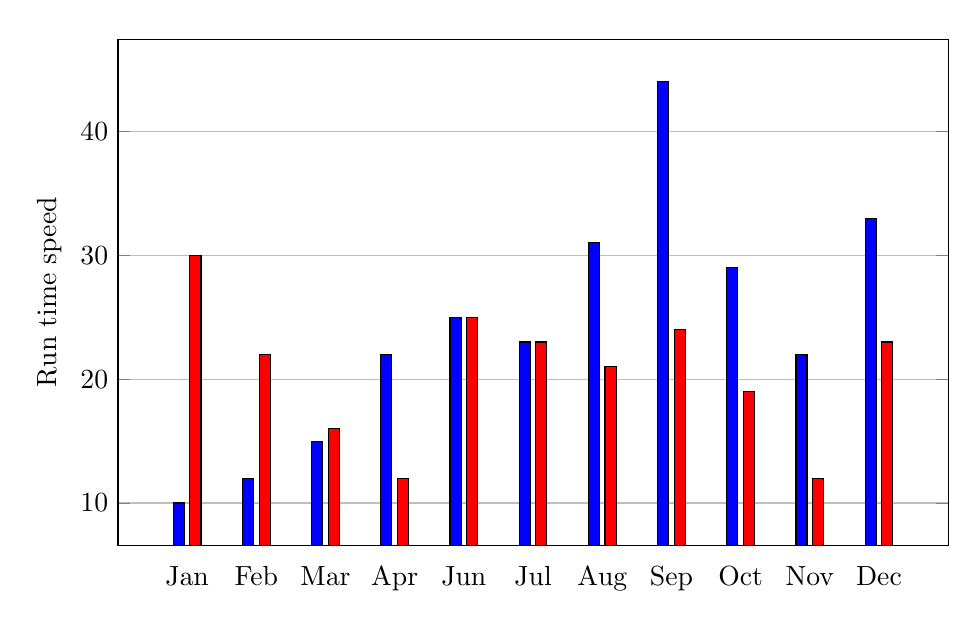
\begin{tikzpicture}	
	\begin{axis} [
	width=1.0\linewidth,      height = 8cm, 
     major x tick style = transparent,
      xtick = data,
	ybar,
	bar width=4pt,
	ymajorgrids = true,
    ylabel = {Run time speed},
       scaled y ticks = false,
    symbolic x coords={Jan, Feb, Mar, Apr, Jun, Jul, Aug, Sep, Oct, Nov, Dec},
	]
	\addplot[ybar,fill=blue] coordinates { (Jan, 10) (Feb, 12) (Mar,15) (Apr,22) (Jun,25) (Jul,23) (Aug,31) (Sep,44) (Oct,29) (Nov,22) (Dec,33) };
	\addplot[ybar,fill=red] coordinates { (Jan, 30) (Feb, 22) (Mar,16) (Apr,12) (Jun,25) (Jul,23) (Aug,21) (Sep,24) (Oct,19) (Nov,12) (Dec,23) };
	\end{axis}
	\end{tikzpicture}
	\caption{Chart name.}
	\label{fig:annu}
	\end{figure}
	figure \ref{fig:annu}.
	
	

	\begin{figure} 
	 \begin{tikzpicture}
		\begin{axis} [
			width=1\linewidth,   height = 8cm, 
		major x tick style = transparent,
		    xtick = data,
		%grid=major, 
		%zeichnet Koordinatengitter
	    symbolic x coords={Jan, Feb, Mar, Apr, May, Jun, Jul, Aug, Sep, Oct, Nov, Dec},
	%	xlabel= Kraft $\lbrack{}$ \si{F} $\rbrack$, 
	%	xmin=0,
	%	xmax=15,
		ylabel= Strom $\lbrack{}$ \si{kA} $\rbrack$,
		ymin=0,	ystep=.25, 	ymax=2.0,
		scaled y ticks = false,
		%nodes near coords, % data 값 표시
		% % % % % Ausrichten der Punktbeschriftung
		every node near coord/.append style={font=\scriptsize,/pgf/number format/precision=3}]
		\addplot table [x=Month, y=2003] {monGAC.csv};
		\addplot table [x=Month, y=2004] {monGAC.csv};
		\addplot table [x=Month, y=2005] {monGAC.csv};
		\addplot table [x=Month, y=2006] {monGAC.csv};
		%   \fill[gray,fill opacity=0.25] (axis cs:5,0) rectangle (axis cs:7,12); %Bereich einfügen
		\end{axis}
		\end{tikzpicture}
		\caption{Chart name.}
			\label{fig:annu}
		\end{figure}
	figure \ref{fig:annu}.

	\begin{figure} 	
 \begin{tikzpicture}
	\begin{axis} [
		width=1\linewidth,   height = 8cm, 
	major x tick style = transparent,
	    xtick = data,
	%grid=major, 
	%zeichnet Koordinatengitter
%    symbolic x coords={Jan, Feb, Mar, Apr, May, Jun, Jul, Aug, Sep, Oct, Nov, Dec},
%	xlabel= Kraft $\lbrack{}$ \si{F} $\rbrack$, 
%	xmin=0,
%	xmax=15,
	ylabel= Strom $\lbrack{}$ \si{kA} $\rbrack$,
	ymin=0,
	ystep=0.5,
	ymax=2.0,
	scaled y ticks = false,
	%nodes near coords, % data 값 표시
	% % % % % Ausrichten der Punktbeschriftung
	every node near coord/.append style={font=\scriptsize,/pgf/number format/precision=3}]
	[legend pos=north east]
	\addplot table [x=Week, y=2003] {wkyGAC.csv}; \addlegendentry{2003}
	\addplot table [x=Week, y=2004] {wkyGAC.csv}; \addlegendentry{2004}
	\addplot table [x=Week, y=2005] {wkyGAC.csv}; \addlegendentry{2005}
	\addplot table [x=Week, y=2006] {wkyGAC.csv}; \addlegendentry{2006}
	%   \fill[gray,fill opacity=0.25] (axis cs:5,0) rectangle (axis cs:7,12); %Bereich einfügen
	\end{axis}
	\end{tikzpicture}
		\caption{Chart name.}
		\label{fig:annu}
	\end{figure}

	figure \ref{fig:annu}.
	

%%%%%%%%%%%%%%%%%%%%%%%%%%%%%%%%%%%%%%%%%%%%%%%%%%%%%%


\begin{figure} 
	\begin{tikzpicture}
	\begin{axis} [
	width=1\linewidth,   height = 6cm, 
	major x tick style = transparent,
	xtick = data,
	%grid=major, 
	%zeichnet Koordinatengitter
   %symbolic x coords={Jan, Feb, Mar, Apr, May, Jun, Jul, Aug, Sep, Oct, Nov, Dec},
	%	xlabel= Kraft $\lbrack{}$ \si{F} $\rbrack$, 
	%	xmin=0,
	%	xmax=15,
	ylabel= chlorophyll-a concentration ($\rm mg/m^3$),
	ymin=0,	ystep=0.5, 	ymax=3.1,
	xmin=0, xstep=4, xmax=47,
	scaled y ticks = false,
	%nodes near coords, % data 값 표시
	% % % % % Ausrichten der Punktbeschriftung
	every node near coord/.append style={font=\scriptsize,/pgf/number format/precision=3}]
	\addplot table [x=Week, y=2003] {wkyLAC.csv}; \addlegendentry{2003}
	\addplot table [x=Week, y=2004] {wkyLAC.csv}; \addlegendentry{2004}
	\addplot table [x=Week, y=2005] {wkyLAC.csv}; \addlegendentry{2005}
	\addplot table [x=Week, y=2006] {wkyLAC.csv}; \addlegendentry{2006}
	%   \fill[gray,fill opacity=0.25] (axis cs:5,0) rectangle (axis cs:7,12); %Bereich einfügen
	\end{axis}
	\end{tikzpicture}

	\begin{tikzpicture}
	\begin{axis} [
	width=1\linewidth,   height = 6cm, 
	major x tick style = transparent,
	xtick = data,
	%grid=major, 
	%zeichnet Koordinatengitter
	%    symbolic x coords={Jan, Feb, Mar, Apr, May, Jun, Jul, Aug, Sep, Oct, Nov, Dec},
	%	xlabel= Kraft $\lbrack{}$ \si{F} $\rbrack$, 
	%	xmin=0,
	%	xmax=15,
	ylabel= chlorophyll-a concentration ($\rm mg/m^3$),
	ymin=0,	ystep=0.5, 	ymax=3.1,
	xmin=0, xstep=4, xmax=47,
	scaled y ticks = false,
	%nodes near coords, % data 값 표시
	% % % % % Ausrichten der Punktbeschriftung
	every node near coord/.append style={font=\scriptsize,/pgf/number format/precision=3}]
	[legend pos=north east]
	\addplot table [x=Week, y=2003] {wkyGAC.csv}; \addlegendentry{2003}
	\addplot table [x=Week, y=2004] {wkyGAC.csv}; \addlegendentry{2004}
	\addplot table [x=Week, y=2005] {wkyGAC.csv}; \addlegendentry{2005}
	\addplot table [x=Week, y=2006] {wkyGAC.csv}; \addlegendentry{2006}
	%   \fill[gray,fill opacity=0.25] (axis cs:5,0) rectangle (axis cs:7,12); %Bereich einfügen
	\end{axis}
	\end{tikzpicture}
	\caption{Chart name.}
	\label{fig:annu}
\end{figure}

figure \ref{fig:annu}.



	
%	
\section{test1}

%%%%%%%%%%%%%%%%%%%%%%%%%%%%%%%%%%%%%%%%%%%%%%%%%%%%%%%%%%%%%%%%%%%%%%%%%%   

\begin{figure}[h]
	\begin{tikzpicture}
	\begin{axis} [
	width=1.0\linewidth,   height = 5cm, 
	major x tick style = transparent,
	xtick = data,
	%grid=major, 
	%zeichnet Koordinatengitter
	symbolic x coords={Jan, Feb, Mar, Apr, May, Jun, Jul, Aug, Sep, Oct, Nov, Dec},
	%	xlabel= Kraft $\lbrack{}$ \si{F} $\rbrack$, 
	%xmin=0, xstep=4, xmax=47,
	ylabel= {\sffamily\small chlorophyll-a concentration ($\rm mg/m^3$)},
	ymin=0,	ystep=0.5, 	ymax=3.1,
	scaled y ticks = false,
	%nodes near coords, % data 값 표시
	% % % % % Ausrichten der Punktbeschriftung
	every node near coord/.append style={font=\scriptsize,/pgf/number format/precision=3}]
	\addplot table [x=Month, y=2003] {./data/monLAC.csv}; \addlegendentry{\sffamily\scriptsize 2003}
	\addplot table [x=Month, y=2004] {./data/monLAC.csv}; \addlegendentry{\sffamily\scriptsize 2004}
	\addplot table [x=Month, y=2005] {./data/monLAC.csv}; \addlegendentry{\sffamily\scriptsize 2005}
	\addplot table [x=Month, y=2006] {./data/monLAC.csv}; \addlegendentry{\sffamily\scriptsize 2006}
	%   \fill[gray,fill opacity=0.25] (axis cs:5,0) rectangle (axis cs:7,12); %Bereich einfügen
	\end{axis}
	\end{tikzpicture}
	
	\begin{tikzpicture}
	\begin{axis} [
	width=1.0\linewidth,   height = 5cm, 
	major x tick style = transparent,
	xtick = data,
	%grid=major, 
	%zeichnet Koordinatengitter
	symbolic x coords={Jan, Feb, Mar, Apr, May, Jun, Jul, Aug, Sep, Oct, Nov, Dec},
	%	xlabel= Kraft $\lbrack{}$ \si{F} $\rbrack$, 
	%	xmin=0,
	%	xmax=15,
	ylabel= {\sffamily\small chlorophyll-a concentration ($\rm mg/m^3$)},
	ymin=0,	ystep=0.5, 	ymax=3.1,
	%xmin=0, xstep=4, xmax=47,
	scaled y ticks = false,
	%nodes near coords, % data 값 표시
	% % % % % Ausrichten der Punktbeschriftung
	every node near coord/.append style={font=\scriptsize,/pgf/number format/precision=3},]
	[legend pos=north east]
	\addplot table [x=Month, y=2003] {./data/monGAC.csv}; \addlegendentry{\sffamily\scriptsize 2003}
	\addplot table [x=Month, y=2004] {./data/monGAC.csv}; \addlegendentry{\sffamily\scriptsize 2004}
	\addplot table [x=Month, y=2005] {./data/monGAC.csv}; \addlegendentry{\sffamily\scriptsize 2005}
	\addplot table [x=Month, y=2006] {./data/monGAC.csv}; \addlegendentry{\sffamily\scriptsize 2006}
	
	%   \fill[gray,fill opacity=0.25] (axis cs:5,0) rectangle (axis cs:7,12); %Bereich einfügen
	\end{axis}
	\end{tikzpicture}
	\caption{The annual variability of monthly-mean chlorophyll-a concentration in the East Sea (Sea of Japan) from 2003 to 2006, (a) LAC (b) GAC.}
	\label{fig:annualmon}
\end{figure}


%%%%%%%%%%%%%%%%%%%%%%%%%%%%%%%%%%%%%%%%%%%%%%%%%%%%%%%%%%%%%%%%%%%%%%%%%%   

\begin{figure}[h]
	\begin{tikzpicture}
	\begin{axis} [
	width=1.0\linewidth,   height = 6cm, 
	major x tick style = transparent,
	xtick = data,
	%grid=major, 
	%zeichnet Koordinatengitter
	symbolic x coords={Jan, Feb, Mar, Apr, May, Jun, Jul, Aug, Sep, Oct, Nov, Dec},
	%	xlabel= Kraft $\lbrack{}$ \si{F} $\rbrack$, 
	%xmin=0, xstep=4, xmax=47,
	ylabel= {\sffamily\small chlorophyll-a concentration ($\rm mg/m^3$)},
	ymin=0,	ystep=0.5, 	ymax=2.1,
	scaled y ticks = false,
	%nodes near coords, % data 값 표시
	% % % % % Ausrichten der Punktbeschriftung
	every node near coord/.append style={font=\scriptsize,/pgf/number format/precision=3}]
	\addplot table [x=Month, y=2003] {./data/monLAC.csv}; \addlegendentry{\sffamily\scriptsize 2003 LAC}
	\addplot table [x=Month, y=2003] {./data/monGAC.csv}; \addlegendentry{\sffamily\scriptsize 2003 GAC}
%   \fill[gray,fill opacity=0.25] (axis cs:5,0) rectangle (axis cs:7,12); %Bereich einfügen
	\end{axis}
	\end{tikzpicture}
	
	\begin{tikzpicture}
	\begin{axis} [
	width=1.0\linewidth,   height = 5cm, 
	major x tick style = transparent,
	xtick = data,
	%grid=major, 
	%zeichnet Koordinatengitter
	symbolic x coords={Jan, Feb, Mar, Apr, May, Jun, Jul, Aug, Sep, Oct, Nov, Dec},
	%	xlabel= Kraft $\lbrack{}$ \si{F} $\rbrack$, 
	%	xmin=0,
	%	xmax=15,
	ylabel= {\sffamily\small difference ($\rm mg/m^3$)},
	ymin=0,	ystep=0.5, 	ymax=2.1,
	%xmin=0, xstep=4, xmax=47,
	scaled y ticks = false,
	%nodes near coords, % data 값 표시
	% % % % % Ausrichten der Punktbeschriftung
	every node near coord/.append style={font=\scriptsize,/pgf/number format/precision=3},]
	[legend pos=north east]
	\addplot table [x=Month, y=2003] {./data/monDIFF.csv}; %\addlegendentry{\sffamily\scriptsize 2003}

	%   \fill[gray,fill opacity=0.25] (axis cs:5,0) rectangle (axis cs:7,12); %Bereich einfügen
	\end{axis}
	\end{tikzpicture}
	\caption{(a) monthly mean values of chlorophyll-a concentration in 2003 using LAC (blue line) and GAC (red line) and (b) its differences between the LAC and GAC data}
	\label{fig:annualmon}
\end{figure}






\begin{figure}[h]
	\begin{tikzpicture}
	\begin{axis} [
	width=1.0\linewidth,   height = 5cm, 
	major x tick style = transparent,
	xtick = data,
	%grid=major, 
	%zeichnet Koordinatengitter
	symbolic x coords={Jan, Feb, Mar, Apr, May, Jun, Jul, Aug, Sep, Oct, Nov, Dec},
	%	xlabel= Kraft $\lbrack{}$ \si{F} $\rbrack$, 
	%xmin=0, xstep=4, xmax=47,
	ylabel= {\sffamily\small chlorophyll-a concentration ($\rm mg/m^3$)},
	ymin=0,	ystep=0.5, 	ymax=3.1,
	scaled y ticks = false,
	%nodes near coords, % data 값 표시
	% % % % % Ausrichten der Punktbeschriftung
	every node near coord/.append style={font=\scriptsize,/pgf/number format/precision=3}]
	\addplot table [x=Month, y=2003] {./data/monLAC.csv}; \addlegendentry{\sffamily\scriptsize 2003}
	\addplot table [x=Month, y=2004] {./data/monLAC.csv}; \addlegendentry{\sffamily\scriptsize 2004}
	\addplot table [x=Month, y=2005] {./data/monLAC.csv}; \addlegendentry{\sffamily\scriptsize 2005}
	\addplot table [x=Month, y=2006] {./data/monLAC.csv}; \addlegendentry{\sffamily\scriptsize 2006}
	%   \fill[gray,fill opacity=0.25] (axis cs:5,0) rectangle (axis cs:7,12); %Bereich einfügen
	\end{axis}
	\end{tikzpicture}
	
	\begin{tikzpicture}
	\begin{axis} [
	  width  = 1.00*\textwidth,
	height = 8cm,
	major x tick style = transparent,
	ybar=2*\pgflinewidth,
	bar width=14pt,
	ymajorgrids = true,
	ylabel = {Run time speed},
	symbolic x coords={EgyptHD,Hover,Navi},
	xtick = data,
	scaled y ticks = false,
	enlarge x limits=0.25,
	ymin=0,
	legend cell align=left,
	legend style={
		at={(1,1.05)},
		anchor=south east,
		column sep=1ex
	}
	]
  \addplot[style={bblue,fill=bblue,mark=none}] table [x=Month, y=2004] {./data/monGAC.csv};

	%   \fill[gray,fill opacity=0.25] (axis cs:5,0) rectangle (axis cs:7,12); %Bereich einfügen
	\end{axis}
	\end{tikzpicture}
	\caption{The annual variability of monthly-mean chlorophyll-a concentration in the East Sea (Sea of Japan) from 2003 to 2006, (a) LAC (b) GAC.}
	\label{fig:annualmon}
\end{figure}



%	\section{test2}

%%%%%%%%%%%%%%%%%%%%%%%%%%%%%%%%%%%%%%%%%%%%%%%%%%%%%%%%%%%%%%%%%%%%%%%%%%   

\begin{figure}[h]
	\begin{tikzpicture}
%	\node [below left,text width=3cm,align=center] at (img.north wast){(a)\footnotemark} % 글자 넣기 위해 추가했으나 에러뜸.
	\begin{axis} [
	width=1.0\linewidth,   height = 6cm, 
	major x tick style = transparent,
	xtick = data,
	%grid=major, 
	symbolic x coords={Jan, Feb, Mar, Apr, May, Jun, Jul, Aug, Sep, Oct, Nov, Dec},
	%	xlabel= Kraft $\lbrack{}$ \si{F} $\rbrack$, 
	%xmin=0, xstep=4, xmax=47,
	ylabel= {\sffamily\small chlorophyll-a concentration ($\rm mg/m^3$)},
	ymin=0,	ystep=0.5, 	ymax=3.1,
	scaled y ticks = false,
	%nodes near coords, % data 값 표시
	% % % % % Ausrichten der Punktbeschriftung
	every node near coord/.append style={font=\scriptsize,/pgf/number format/precision=3}]
	\addplot table [x=Month, y=2003] {./data/monLAC.csv}; \addlegendentry{\sffamily\scriptsize 2003}
	\addplot table [x=Month, y=2004] {./data/monLAC.csv}; \addlegendentry{\sffamily\scriptsize 2004}
	\addplot table [x=Month, y=2005] {./data/monLAC.csv}; \addlegendentry{\sffamily\scriptsize 2005}
	\addplot table [x=Month, y=2006] {./data/monLAC.csv}; \addlegendentry{\sffamily\scriptsize 2006}
	%   \fill[gray,fill opacity=0.25] (axis cs:5,0) rectangle (axis cs:7,12); %Bereich einfügen
	\end{axis}
	\end{tikzpicture}
	
	\begin{tikzpicture}
	\begin{axis} [
	width=1.0\linewidth,   height = 6cm, 
	major x tick style = transparent,
	xtick = data,
	%grid=major, 
	symbolic x coords={Jan, Feb, Mar, Apr, May, Jun, Jul, Aug, Sep, Oct, Nov, Dec},
	%	xlabel= Kraft $\lbrack{}$ \si{F} $\rbrack$, 
	%	xmin=0,
	%	xmax=15,
	ylabel= {\sffamily\small chlorophyll-a concentration ($\rm mg/m^3$)},
	ymin=0,	ystep=0.5, 	ymax=3.1,
	%xmin=0, xstep=4, xmax=47,
	scaled y ticks = false,
	%nodes near coords, % data 값 표시
	% % % % % Ausrichten der Punktbeschriftung
	every node near coord/.append style={font=\scriptsize,/pgf/number format/precision=3},]
	[legend pos=north east]
	\addplot table [x=Month, y=2003] {./data/monGAC.csv}; \addlegendentry{\sffamily\scriptsize 2003}
	\addplot table [x=Month, y=2004] {./data/monGAC.csv}; \addlegendentry{\sffamily\scriptsize 2004}
	\addplot table [x=Month, y=2005] {./data/monGAC.csv}; \addlegendentry{\sffamily\scriptsize 2005}
	\addplot table [x=Month, y=2006] {./data/monGAC.csv}; \addlegendentry{\sffamily\scriptsize 2006}
	
	%   \fill[gray,fill opacity=0.25] (axis cs:5,0) rectangle (axis cs:7,12); %Bereich einfügen
	\end{axis}
	\end{tikzpicture}
	\caption{The annual variability of monthly-mean chlorophyll-a concentration in the East Sea (Sea of Japan) from 2003 to 2006, (a) LAC (b) GAC.}
	\label{fig:annualmon}
\end{figure}


%%%%%%%%%%%%%%%%%%%%%%%%%%%%%%%%%%%%%%%%%%%%%%%%%%%%%%%%%%%%%%%%%%%%%%%%%%   

\begin{figure}[h]
	\begin{tikzpicture}
	\begin{axis} [
	width=1.0\linewidth,   height = 6cm, 
	major x tick style = transparent,
	xtick = data,
	%grid=major, 
	symbolic x coords={Jan, Feb, Mar, Apr, May, Jun, Jul, Aug, Sep, Oct, Nov, Dec},
	%	xlabel= Kraft $\lbrack{}$ \si{F} $\rbrack$, 
	%xmin=0, xstep=4, xmax=47,
	ylabel= {\sffamily\small chlorophyll-a concentration ($\rm mg/m^3$)},
	ymin=0,	ystep=0.5, 	ymax=2.1,
	scaled y ticks = false,
	%nodes near coords, % data 값 표시
	% % % % % Ausrichten der Punktbeschriftung
	every node near coord/.append style={font=\scriptsize,/pgf/number format/precision=3}]
	\addplot table [x=Month, y=2003] {./data/monLAC.csv}; \addlegendentry{\sffamily\scriptsize 2003 LAC}
	\addplot table [x=Month, y=2003] {./data/monGAC.csv}; \addlegendentry{\sffamily\scriptsize 2003 GAC}
	%   \fill[gray,fill opacity=0.25] (axis cs:5,0) rectangle (axis cs:7,12); %Bereich einfügen
	\end{axis}
	\end{tikzpicture}
	
	\begin{tikzpicture}
	\begin{axis} [
	width=1.0\linewidth,   height = 6cm, 
	major x tick style = transparent,
	xtick = data,
	%grid=major, 
	symbolic x coords={Jan, Feb, Mar, Apr, May, Jun, Jul, Aug, Sep, Oct, Nov, Dec},
	%	xlabel= Kraft $\lbrack{}$ \si{F} $\rbrack$, 
	%	xmin=0,
	%	xmax=15,
	ylabel= {\sffamily\small difference ($\rm mg/m^3$)},
	ymin=-0.2,	ystep=0.1, 	ymax=0.2,
	%xmin=0, xstep=4, xmax=47,
	scaled y ticks = false,
	%nodes near coords, % data 값 표시
	% % % % % Ausrichten der Punktbeschriftung
	every node near coord/.append style={font=\scriptsize,/pgf/number format/precision=3},]
	[legend pos=north east]
	\addplot table [x=Month, y=2003] {./data/monDIFF.csv}; %\addlegendentry{\sffamily\scriptsize 2003}
	
	%   \fill[gray,fill opacity=0.25] (axis cs:5,0) rectangle (axis cs:7,12); %Bereich einfügen
	\end{axis}
	\end{tikzpicture}
	\caption{(a) monthly mean values of chlorophyll-a concentration in 2003 using LAC (blue line) and GAC (red line) and (b) its differences between the LAC and GAC data}
	\label{fig:annualmon}
\end{figure}

%%%%%%%%%%%%%%%%%%%%%%%%%%%%%%%%%%%%%%%%%%%%%%%%%%%%%%%%%%%%%%%%%%%%%%%%%%   

\begin{figure}[h]
	\begin{tikzpicture}
	\begin{axis} [
	width=1.0\linewidth,   height = 6cm, 
	major x tick style = transparent,
	xtick = data,
	%grid=major, 
	symbolic x coords={Jan, Feb, Mar, Apr, May, Jun, Jul, Aug, Sep, Oct, Nov, Dec},
	%	xlabel= Kraft $\lbrack{}$ \si{F} $\rbrack$, 
	%xmin=0, xstep=4, xmax=47,
	ylabel= {\sffamily\small chlorophyll-a concentration ($\rm mg/m^3$)},
	ymin=0,	ystep=0.5, 	ymax=2.1,
	scaled y ticks = false,
	%nodes near coords, % data 값 표시
	% % % % % Ausrichten der Punktbeschriftung
	every node near coord/.append style={font=\scriptsize,/pgf/number format/precision=3}]
	\addplot table [x=Month, y=2003] {./data/monLAC.csv}; \addlegendentry{\sffamily\scriptsize 2003 LAC}
	\addplot table [x=Month, y=2003] {./data/monGAC.csv}; \addlegendentry{\sffamily\scriptsize 2003 GAC}
	%   \fill[gray,fill opacity=0.25] (axis cs:5,0) rectangle (axis cs:7,12); %Bereich einfügen
	\end{axis}
	\end{tikzpicture}
	
	\begin{tikzpicture}
	\begin{axis} [
	width=1.0\linewidth,   height = 4cm, 
	major x tick style = transparent,
	xtick = data,
	%grid=major, 
	symbolic x coords={Jan, Feb, Mar, Apr, May, Jun, Jul, Aug, Sep, Oct, Nov, Dec},
	%	xlabel= Kraft $\lbrack{}$ \si{F} $\rbrack$, 
	%	xmin=0,
	%	xmax=15,
	ylabel= {\sffamily\small difference ($\rm mg/m^3$)},
	ymin=-0.2,	ystep=0.1, 	ymax=0.2,
	%xmin=0, xstep=4, xmax=47,
	scaled y ticks = false,
	%nodes near coords, % data 값 표시
	% % % % % Ausrichten der Punktbeschriftung
	every node near coord/.append style={font=\scriptsize,/pgf/number format/precision=3},]
	[legend pos=north east]
	\addplot table [x=Month, y=2003] {./data/monDIFF.csv}; %\addlegendentry{\sffamily\scriptsize 2003}
	
	%   \fill[gray,fill opacity=0.25] (axis cs:5,0) rectangle (axis cs:7,12); %Bereich einfügen
	\end{axis}
	\end{tikzpicture}
	
	\begin{tikzpicture}
	\begin{axis} [
	width=1.0\linewidth,   height = 6cm, 
	major x tick style = transparent,
	xtick = data,
	%grid=major, 
	symbolic x coords={Jan, Feb, Mar, Apr, May, Jun, Jul, Aug, Sep, Oct, Nov, Dec},
	%	xlabel= Kraft $\lbrack{}$ \si{F} $\rbrack$, 
	%xmin=0, xstep=4, xmax=47,
	ylabel= {\sffamily\small chlorophyll-a concentration ($\rm mg/m^3$)},
	ymin=0,	ystep=0.5, 	ymax=2.1,
	scaled y ticks = false,
	%nodes near coords, % data 값 표시
	% % % % % Ausrichten der Punktbeschriftung
	every node near coord/.append style={font=\scriptsize,/pgf/number format/precision=3}]
	\addplot table [x=Month, y=2004] {./data/monLAC.csv}; \addlegendentry{\sffamily\scriptsize 2004 LAC}
	\addplot table [x=Month, y=2004] {./data/monGAC.csv}; \addlegendentry{\sffamily\scriptsize 2004 GAC}
	%   \fill[gray,fill opacity=0.25] (axis cs:5,0) rectangle (axis cs:7,12); %Bereich einfügen
	\end{axis}
	\end{tikzpicture}
	
	\begin{tikzpicture}
	\begin{axis} [
	width=1.0\linewidth,   height = 4cm, 
	major x tick style = transparent,
	xtick = data,
	%grid=major, 
	symbolic x coords={Jan, Feb, Mar, Apr, May, Jun, Jul, Aug, Sep, Oct, Nov, Dec},
	%	xlabel= Kraft $\lbrack{}$ \si{F} $\rbrack$, 
	%	xmin=0,
	%	xmax=15,
	ylabel= {\sffamily\small difference ($\rm mg/m^3$)},
	ymin=-0.2,	ystep=0.1, 	ymax=0.2,
	%xmin=0, xstep=4, xmax=47,
	scaled y ticks = false,
	%nodes near coords, % data 값 표시
	% % % % % Ausrichten der Punktbeschriftung
	every node near coord/.append style={font=\scriptsize,/pgf/number format/precision=3},]
	[legend pos=north east]
	\addplot table [x=Month, y=2004] {./data/monDIFF.csv}; %\addlegendentry{\sffamily\scriptsize 2003}
	
	%   \fill[gray,fill opacity=0.25] (axis cs:5,0) rectangle (axis cs:7,12); %Bereich einfügen
	\end{axis}
	\end{tikzpicture}
	
	
	\caption{(a) monthly mean values of chlorophyll-a concentration in 2003 using LAC (blue line) and GAC (red line) and (b) its differences between the LAC and GAC data}
	\label{fig:annualmon}
\end{figure}


%%%%%%%%%%%%%%%%%%%%%%%%%%%%%%%%%%%%%%%%%%%%%%%%%%%%%%%%%%%%%%%%%%%%%%%%%%   

\begin{figure}[h]
	
	\begin{tikzpicture}
	\begin{axis} [
	width=1.0\linewidth,   height = 6cm, 
	major x tick style = transparent,
	xtick = data,
	%grid=major, 
	symbolic x coords={Jan, Feb, Mar, Apr, May, Jun, Jul, Aug, Sep, Oct, Nov, Dec},
	%	xlabel= Kraft $\lbrack{}$ \si{F} $\rbrack$, 
	%xmin=0, xstep=4, xmax=47,
	ylabel= {\sffamily\small chlorophyll-a concentration ($\rm mg/m^3$)},
	ymin=0,	ystep=0.5, 	ymax=2.1,
	scaled y ticks = false,
	%nodes near coords, % data 값 표시
	% % % % % Ausrichten der Punktbeschriftung
	every node near coord/.append style={font=\sffamily\scriptsize,/pgf/number format/precision=3}]
	\addplot table [x=Month, y=2005] {./data/monLAC.csv}; \addlegendentry{\sffamily\scriptsize 2005 LAC}
	\addplot table [x=Month, y=2005] {./data/monGAC.csv}; \addlegendentry{\sffamily\scriptsize 2005 GAC}
	%   \fill[gray,fill opacity=0.25] (axis cs:5,0) rectangle (axis cs:7,12); %Bereich einfügen
	\end{axis}
	\end{tikzpicture}
	
	\begin{tikzpicture}
	\begin{axis} [
	width=1.0\linewidth,   height = 4cm, 
	major x tick style = transparent,
	xtick = data,
	%grid=major, 
	symbolic x coords={Jan, Feb, Mar, Apr, May, Jun, Jul, Aug, Sep, Oct, Nov, Dec},
	%	xlabel= Kraft $\lbrack{}$ \si{F} $\rbrack$, 
	%	xmin=0,
	%	xmax=15,
	ylabel= {\sffamily\small difference ($\rm mg/m^3$)},
	ymin=-0.2,	ystep=0.1, 	ymax=0.2,
	%xmin=0, xstep=4, xmax=47,
	scaled y ticks = false,
	%nodes near coords, % data 값 표시
	% % % % % Ausrichten der Punktbeschriftung
	every node near coord/.append style={font=\scriptsize,/pgf/number format/precision=3},]
	[legend pos=north east]
	\addplot table [x=Month, y=2005] {./data/monDIFF.csv}; %\addlegendentry{\sffamily\scriptsize 2003}
	
	%   \fill[gray,fill opacity=0.25] (axis cs:5,0) rectangle (axis cs:7,12); %Bereich einfügen
	\end{axis}
	\end{tikzpicture}
	
	\begin{tikzpicture}
	\begin{axis} [
	width=1.0\linewidth,   height = 6cm, 
	major x tick style = transparent,
	xtick = data,
	%grid=major, 
	symbolic x coords={Jan, Feb, Mar, Apr, May, Jun, Jul, Aug, Sep, Oct, Nov, Dec},
	%	xlabel= Kraft $\lbrack{}$ \si{F} $\rbrack$, 
	%xmin=0, xstep=4, xmax=47,
	ylabel= {\sffamily\small chlorophyll-a concentration ($\rm mg/m^3$)},
	ymin=0,	ystep=0.5, 	ymax=2.1,
	scaled y ticks = false,
	%nodes near coords, % data 값 표시
	% % % % % Ausrichten der Punktbeschriftung
	every node near coord/.append style={font=\sffamily\scriptsize,/pgf/number format/precision=3}]
	\addplot table [x=Month, y=2006] {./data/monLAC.csv}; \addlegendentry{\sffamily\scriptsize 2006 LAC}
	\addplot table [x=Month, y=2006] {./data/monGAC.csv}; \addlegendentry{\sffamily\scriptsize 2006 GAC}
	\end{axis}
	\end{tikzpicture}
	
	\begin{tikzpicture}
	\begin{axis} [
	width=1.0\linewidth,   height = 4cm, 
	major x tick style = transparent,
	xtick = data,
	%grid=major, 
	symbolic x coords={Jan, Feb, Mar, Apr, May, Jun, Jul, Aug, Sep, Oct, Nov, Dec},
	%	xlabel= Kraft $\lbrack{}$ \si{F} $\rbrack$, 
	%	xmin=0,
	%	xmax=15,
	ylabel= {\sffamily\small difference ($\rm mg/m^3$)},
	ymin=-0.2,	ystep=0.1, 	ymax=0.2,
	%xmin=0, xstep=4, xmax=47,
	scaled y ticks = false,
	%nodes near coords, % data 값 표시
	% % % % % Ausrichten der Punktbeschriftung
	every node near coord/.append style={font=\scriptsize,/pgf/number format/precision=3},]
	[legend pos=north east]
	\addplot table [x=Month, y=2006] {./data/monDIFF.csv}; %\addlegendentry{\sffamily\scriptsize 2003}
	
	%   \fill[gray,fill opacity=0.25] (axis cs:5,0) rectangle (axis cs:7,12); %Bereich einfügen
	\end{axis}
	\end{tikzpicture}
	
	\caption{(a) monthly mean values of chlorophyll-a concentration in 2003 using LAC (blue line) and GAC (red line) and (b) its differences between the LAC and GAC data}
	\label{fig:annualmon}
\end{figure}


%	\section{test}

%%%%%%%%%%%%%%%%%%%%%%%%%%%%%%%%%%%%%%%%%%%%%%%%%%%%%%%%%%%%%%%%%%%%%%%%%%   

\begin{figure}[h]
	\begin{tikzpicture}
%	\node [below left,text width=3cm,align=center] at (img.north wast){(a)\footnotemark} % 글자 넣기 위해 추가했으나 에러뜸.
	\begin{axis} [
	width=1.0\linewidth,   height = 6cm, 
	major x tick style = transparent,
	xtick = data,
	%grid=major, 
	symbolic x coords={Jan, Feb, Mar, Apr, May, Jun, Jul, Aug, Sep, Oct, Nov, Dec},
	%	xlabel= Kraft $\lbrack{}$ \si{F} $\rbrack$, 
	%xmin=0, xstep=4, xmax=47,
	ylabel= {\sffamily\small chlorophyll-a concentration ($\rm mg/m^3$)},
	ymin=0,	ystep=0.5, 	ymax=3.1,
	scaled y ticks = false,
	%nodes near coords, % data 값 표시
	% % % % % Ausrichten der Punktbeschriftung
	every node near coord/.append style={font=\scriptsize,/pgf/number format/precision=3}]
	\addplot table [x=Month, y=2003] {./data/monLAC.csv}; \addlegendentry{\sffamily\scriptsize 2003}
	\addplot table [x=Month, y=2004] {./data/monLAC.csv}; \addlegendentry{\sffamily\scriptsize 2004}
	\addplot table [x=Month, y=2005] {./data/monLAC.csv}; \addlegendentry{\sffamily\scriptsize 2005}
	\addplot table [x=Month, y=2006] {./data/monLAC.csv}; \addlegendentry{\sffamily\scriptsize 2006}
	%   \fill[gray,fill opacity=0.25] (axis cs:5,0) rectangle (axis cs:7,12); %Bereich einfügen
	\end{axis}
	\end{tikzpicture}
	
	\begin{tikzpicture}
	\begin{axis} [
	width=1.0\linewidth,   height = 6cm, 
	major x tick style = transparent,
	xtick = data,
	%grid=major, 
	symbolic x coords={Jan, Feb, Mar, Apr, May, Jun, Jul, Aug, Sep, Oct, Nov, Dec},
	%	xlabel= Kraft $\lbrack{}$ \si{F} $\rbrack$, 
	%	xmin=0,
	%	xmax=15,
	ylabel= {\sffamily\small chlorophyll-a concentration ($\rm mg/m^3$)},
	ymin=0,	ystep=0.5, 	ymax=3.1,
	%xmin=0, xstep=4, xmax=47,
	scaled y ticks = false,
	%nodes near coords, % data 값 표시
	% % % % % Ausrichten der Punktbeschriftung
	every node near coord/.append style={font=\scriptsize,/pgf/number format/precision=3},]
	[legend pos=north east]
	\addplot table [x=Month, y=2003] {./data/monGAC.csv}; \addlegendentry{\sffamily\scriptsize 2003}
	\addplot table [x=Month, y=2004] {./data/monGAC.csv}; \addlegendentry{\sffamily\scriptsize 2004}
	\addplot table [x=Month, y=2005] {./data/monGAC.csv}; \addlegendentry{\sffamily\scriptsize 2005}
	\addplot table [x=Month, y=2006] {./data/monGAC.csv}; \addlegendentry{\sffamily\scriptsize 2006}
	
	%   \fill[gray,fill opacity=0.25] (axis cs:5,0) rectangle (axis cs:7,12); %Bereich einfügen
	\end{axis}
	\end{tikzpicture}
	\caption{The annual variability of monthly-mean chlorophyll-a concentration in the East Sea (Sea of Japan) from 2003 to 2006, (a) LAC (b) GAC.}
	\label{fig:annualmon}
\end{figure}


%%%%%%%%%%%%%%%%%%%%%%%%%%%%%%%%%%%%%%%%%%%%%%%%%%%%%%%%%%%%%%%%%%%%%%%%%%   

\begin{figure}[h]
	\begin{tikzpicture}
	\begin{axis} [
	width=1.0\linewidth,   height = 6cm, 
	major x tick style = transparent,
	xtick = data,
	%grid=major, 
	symbolic x coords={Jan, Feb, Mar, Apr, May, Jun, Jul, Aug, Sep, Oct, Nov, Dec},
	%	xlabel= Kraft $\lbrack{}$ \si{F} $\rbrack$, 
	%xmin=0, xstep=4, xmax=47,
	ylabel= {\sffamily\small chlorophyll-a concentration ($\rm mg/m^3$)},
	ymin=0,	ystep=0.5, 	ymax=2.1,
	scaled y ticks = false,
	%nodes near coords, % data 값 표시
	% % % % % Ausrichten der Punktbeschriftung
	every node near coord/.append style={font=\scriptsize,/pgf/number format/precision=3}]
	\addplot table [x=Month, y=2003] {./data/monLAC.csv}; \addlegendentry{\sffamily\scriptsize 2003 LAC}
	\addplot table [x=Month, y=2003] {./data/monGAC.csv}; \addlegendentry{\sffamily\scriptsize 2003 GAC}
	%   \fill[gray,fill opacity=0.25] (axis cs:5,0) rectangle (axis cs:7,12); %Bereich einfügen
	\end{axis}
	\end{tikzpicture}
	
	\begin{tikzpicture}
	\begin{axis} [
	width=1.0\linewidth,   height = 6cm, 
	major x tick style = transparent,
	xtick = data,
	%grid=major, 
	symbolic x coords={Jan, Feb, Mar, Apr, May, Jun, Jul, Aug, Sep, Oct, Nov, Dec},
	%	xlabel= Kraft $\lbrack{}$ \si{F} $\rbrack$, 
	%	xmin=0,
	%	xmax=15,
	ylabel= {\sffamily\small difference ($\rm mg/m^3$)},
	ymin=-0.2,	ystep=0.1, 	ymax=0.2,
	%xmin=0, xstep=4, xmax=47,
	scaled y ticks = false,
	%nodes near coords, % data 값 표시
	% % % % % Ausrichten der Punktbeschriftung
	every node near coord/.append style={font=\scriptsize,/pgf/number format/precision=3},]
	[legend pos=north east]
	\addplot table [x=Month, y=2003] {./data/monDIFF.csv}; %\addlegendentry{\sffamily\scriptsize 2003}
	
	%   \fill[gray,fill opacity=0.25] (axis cs:5,0) rectangle (axis cs:7,12); %Bereich einfügen
	\end{axis}
	\end{tikzpicture}
	\caption{(a) monthly mean values of chlorophyll-a concentration in 2003 using LAC (blue line) and GAC (red line) and (b) its differences between the LAC and GAC data}
	\label{fig:annualmon}
\end{figure}

%%%%%%%%%%%%%%%%%%%%%%%%%%%%%%%%%%%%%%%%%%%%%%%%%%%%%%%%%%%%%%%%%%%%%%%%%%   

\begin{figure}[h]
	\begin{tikzpicture}
	\begin{axis} [
	width=1.0\linewidth,   height = 6cm, 
	major x tick style = transparent,
	xtick = data,
	%grid=major, 
	symbolic x coords={Jan, Feb, Mar, Apr, May, Jun, Jul, Aug, Sep, Oct, Nov, Dec},
	%	xlabel= Kraft $\lbrack{}$ \si{F} $\rbrack$, 
	%xmin=0, xstep=4, xmax=47,
	ylabel= {\sffamily\small chlorophyll-a concentration ($\rm mg/m^3$)},
	ymin=0,	ystep=0.5, 	ymax=2.1,
	scaled y ticks = false,
	%nodes near coords, % data 값 표시
	% % % % % Ausrichten der Punktbeschriftung
	every node near coord/.append style={font=\scriptsize,/pgf/number format/precision=3}]
	\addplot table [x=Month, y=2003] {./data/monLAC.csv}; \addlegendentry{\sffamily\scriptsize 2003 LAC}
	\addplot table [x=Month, y=2003] {./data/monGAC.csv}; \addlegendentry{\sffamily\scriptsize 2003 GAC}
	%   \fill[gray,fill opacity=0.25] (axis cs:5,0) rectangle (axis cs:7,12); %Bereich einfügen
	\end{axis}
	\end{tikzpicture}
	
	\begin{tikzpicture}
	\begin{axis} [
	width=1.0\linewidth,   height = 4cm, 
	major x tick style = transparent,
	xtick = data,
	%grid=major, 
	symbolic x coords={Jan, Feb, Mar, Apr, May, Jun, Jul, Aug, Sep, Oct, Nov, Dec},
	%	xlabel= Kraft $\lbrack{}$ \si{F} $\rbrack$, 
	%	xmin=0,
	%	xmax=15,
	ylabel= {\sffamily\small difference ($\rm mg/m^3$)},
	ymin=-0.2,	ystep=0.1, 	ymax=0.2,
	%xmin=0, xstep=4, xmax=47,
	scaled y ticks = false,
	%nodes near coords, % data 값 표시
	% % % % % Ausrichten der Punktbeschriftung
	every node near coord/.append style={font=\scriptsize,/pgf/number format/precision=3},]
	[legend pos=north east]
	\addplot table [x=Month, y=2003] {./data/monDIFF.csv}; %\addlegendentry{\sffamily\scriptsize 2003}
	
	%   \fill[gray,fill opacity=0.25] (axis cs:5,0) rectangle (axis cs:7,12); %Bereich einfügen
	\end{axis}
	\end{tikzpicture}
	
	\begin{tikzpicture}
	\begin{axis} [
	width=1.0\linewidth,   height = 6cm, 
	major x tick style = transparent,
	xtick = data,
	%grid=major, 
	symbolic x coords={Jan, Feb, Mar, Apr, May, Jun, Jul, Aug, Sep, Oct, Nov, Dec},
	%	xlabel= Kraft $\lbrack{}$ \si{F} $\rbrack$, 
	%xmin=0, xstep=4, xmax=47,
	ylabel= {\sffamily\small chlorophyll-a concentration ($\rm mg/m^3$)},
	ymin=0,	ystep=0.5, 	ymax=2.1,
	scaled y ticks = false,
	%nodes near coords, % data 값 표시
	% % % % % Ausrichten der Punktbeschriftung
	every node near coord/.append style={font=\scriptsize,/pgf/number format/precision=3}]
	\addplot table [x=Month, y=2004] {./data/monLAC.csv}; \addlegendentry{\sffamily\scriptsize 2004 LAC}
	\addplot table [x=Month, y=2004] {./data/monGAC.csv}; \addlegendentry{\sffamily\scriptsize 2004 GAC}
	%   \fill[gray,fill opacity=0.25] (axis cs:5,0) rectangle (axis cs:7,12); %Bereich einfügen
	\end{axis}
	\end{tikzpicture}
	
	\begin{tikzpicture}
	\begin{axis} [
	width=1.0\linewidth,   height = 4cm, 
	major x tick style = transparent,
	xtick = data,
	%grid=major, 
	symbolic x coords={Jan, Feb, Mar, Apr, May, Jun, Jul, Aug, Sep, Oct, Nov, Dec},
	%	xlabel= Kraft $\lbrack{}$ \si{F} $\rbrack$, 
	%	xmin=0,
	%	xmax=15,
	ylabel= {\sffamily\small difference ($\rm mg/m^3$)},
	ymin=-0.2,	ystep=0.1, 	ymax=0.2,
	%xmin=0, xstep=4, xmax=47,
	scaled y ticks = false,
	%nodes near coords, % data 값 표시
	% % % % % Ausrichten der Punktbeschriftung
	every node near coord/.append style={font=\scriptsize,/pgf/number format/precision=3},]
	[legend pos=north east]
	\addplot table [x=Month, y=2004] {./data/monDIFF.csv}; %\addlegendentry{\sffamily\scriptsize 2003}
	
	%   \fill[gray,fill opacity=0.25] (axis cs:5,0) rectangle (axis cs:7,12); %Bereich einfügen
	\end{axis}
	\end{tikzpicture}
	
	
	\caption{(a) monthly mean values of chlorophyll-a concentration in 2003 using LAC (blue line) and GAC (red line) and (b) its differences between the LAC and GAC data}
	\label{fig:annualmon}
\end{figure}


%%%%%%%%%%%%%%%%%%%%%%%%%%%%%%%%%%%%%%%%%%%%%%%%%%%%%%%%%%%%%%%%%%%%%%%%%%   

\begin{figure}[h]
	
	\begin{tikzpicture}
	\begin{axis} [
	width=1.0\linewidth,   height = 6cm, 
	major x tick style = transparent,
	xtick = data,
	%grid=major, 
	symbolic x coords={Jan, Feb, Mar, Apr, May, Jun, Jul, Aug, Sep, Oct, Nov, Dec},
	%	xlabel= Kraft $\lbrack{}$ \si{F} $\rbrack$, 
	%xmin=0, xstep=4, xmax=47,
	ylabel= {\sffamily\small chlorophyll-a concentration ($\rm mg/m^3$)},
	ymin=0,	ystep=0.5, 	ymax=2.1,
	scaled y ticks = false,
	%nodes near coords, % data 값 표시
	% % % % % Ausrichten der Punktbeschriftung
	every node near coord/.append style={font=\sffamily\scriptsize,/pgf/number format/precision=3}]
	\addplot table [x=Month, y=2005] {./data/monLAC.csv}; \addlegendentry{\sffamily\scriptsize 2005 LAC}
	\addplot table [x=Month, y=2005] {./data/monGAC.csv}; \addlegendentry{\sffamily\scriptsize 2005 GAC}
	%   \fill[gray,fill opacity=0.25] (axis cs:5,0) rectangle (axis cs:7,12); %Bereich einfügen
	\end{axis}
	\end{tikzpicture}
	
	\begin{tikzpicture}
	\begin{axis} [
	width=1.0\linewidth,   height = 4cm, 
	major x tick style = transparent,
	xtick = data,
	%grid=major, 
	symbolic x coords={Jan, Feb, Mar, Apr, May, Jun, Jul, Aug, Sep, Oct, Nov, Dec},
	%	xlabel= Kraft $\lbrack{}$ \si{F} $\rbrack$, 
	%	xmin=0,
	%	xmax=15,
	ylabel= {\sffamily\small difference ($\rm mg/m^3$)},
	ymin=-0.2,	ystep=0.1, 	ymax=0.2,
	%xmin=0, xstep=4, xmax=47,
	scaled y ticks = false,
	%nodes near coords, % data 값 표시
	% % % % % Ausrichten der Punktbeschriftung
	every node near coord/.append style={font=\scriptsize,/pgf/number format/precision=3},]
	[legend pos=north east]
	\addplot table [x=Month, y=2005] {./data/monDIFF.csv}; %\addlegendentry{\sffamily\scriptsize 2003}
	
	%   \fill[gray,fill opacity=0.25] (axis cs:5,0) rectangle (axis cs:7,12); %Bereich einfügen
	\end{axis}
	\end{tikzpicture}
	
	\begin{tikzpicture}
	\begin{axis} [
	width=1.0\linewidth,   height = 6cm, 
	major x tick style = transparent,
	xtick = data,
	%grid=major, 
	symbolic x coords={Jan, Feb, Mar, Apr, May, Jun, Jul, Aug, Sep, Oct, Nov, Dec},
	%	xlabel= Kraft $\lbrack{}$ \si{F} $\rbrack$, 
	%xmin=0, xstep=4, xmax=47,
	ylabel= {\sffamily\small chlorophyll-a concentration ($\rm mg/m^3$)},
	ymin=0,	ystep=0.5, 	ymax=2.1,
	scaled y ticks = false,
	%nodes near coords, % data 값 표시
	% % % % % Ausrichten der Punktbeschriftung
	every node near coord/.append style={font=\sffamily\scriptsize,/pgf/number format/precision=3}]
	\addplot table [x=Month, y=2006] {./data/monLAC.csv}; \addlegendentry{\sffamily\scriptsize 2006 LAC}
	\addplot table [x=Month, y=2006] {./data/monGAC.csv}; \addlegendentry{\sffamily\scriptsize 2006 GAC}
	\end{axis}
	\end{tikzpicture}
	
	\begin{tikzpicture}
	\begin{axis} [
	width=1.0\linewidth,   height = 4cm, 
	major x tick style = transparent,
	xtick = data,
	%grid=major, 
	symbolic x coords={Jan, Feb, Mar, Apr, May, Jun, Jul, Aug, Sep, Oct, Nov, Dec},
	%	xlabel= Kraft $\lbrack{}$ \si{F} $\rbrack$, 
	%	xmin=0,
	%	xmax=15,
	ylabel= {\sffamily\small difference ($\rm mg/m^3$)},
	ymin=-0.2,	ystep=0.1, 	ymax=0.2,
	%xmin=0, xstep=4, xmax=47,
	scaled y ticks = false,
	%nodes near coords, % data 값 표시
	% % % % % Ausrichten der Punktbeschriftung
	every node near coord/.append style={font=\scriptsize,/pgf/number format/precision=3},]
	[legend pos=north east]
	\addplot table [x=Month, y=2006] {./data/monDIFF.csv}; %\addlegendentry{\sffamily\scriptsize 2003}
	
	%   \fill[gray,fill opacity=0.25] (axis cs:5,0) rectangle (axis cs:7,12); %Bereich einfügen
	\end{axis}
	\end{tikzpicture}
	
	\caption{(a) monthly mean values of chlorophyll-a concentration in 2003 using LAC (blue line) and GAC (red line) and (b) its differences between the LAC and GAC data}
	\label{fig:annualmon}
\end{figure}


%	\section{test4}


%%%%%%%%%%%%%%%%%%%%%%%%%%%%%%%%%%%%%%%%%%%%%%%%%%%%%%%%%%%%%%%%%%%%%%%%%%   
%4-1 4-1 4-1 4-1

\begin{figure}[h]
	\begin{tikzpicture}
	%	\node [below left,text width=3cm,align=center] at (img.north wast){(a)\footnotemark} % 글자 넣기 위해 추가했으나 에러뜸.
	\begin{axis} [
	width=1.0\linewidth,   height = 6cm, 
	major x tick style = transparent,
%xtick = data,
xtick = {03Jan, , , , , , 03Jul, , , , , ,
	04Jan, , , , , , 04Jul, , , , , ,
	05Jan, , , , , , 05Jul, , , , , ,
	06Jan, , , , , , 06Jul, , , , , 06Dec},
	%grid=major, 
	symbolic x coords={	03Jan, 03Feb, 03Mar, 03Apr, 03May, 03Jun, 03Jul, 03Aug, 03Sep, 03Oct, 03Nov, 03Dec,
		04Jan, 04Feb, 04Mar, 04Apr, 04May, 04Jun, 04Jul, 04Aug, 04Sep, 04Oct, 04Nov,  04Dec, 
		05Jan, 05Feb,05Mar, 05Apr, 05May, 05Jun, 05Jul, 05Aug, 05Sep, 05Oct, 05Nov, 		05Dec,
		06Jan, 06Feb, 06Mar, 06Apr, 06May, 06Jun, 06Jul, 06Aug, 06Sep, 06Oct, 06Nov, 06Dec
	},
	%	xlabel= Kraft $\lbrack{}$ \si{F} $\rbrack$, 
	%xmin=0, xstep=4, xmax=47,
	ylabel= {\sffamily\small chlorophyll-a concentration ($\rm mg/m^3$)},
	ymin=0,	ystep=0.5, 	ymax=4.1,
	scaled y ticks = false,
	%nodes near coords, % data 값 표시
	% % % % % Ausrichten der Punktbeschriftung
	every node near coord/.append style={font=\scriptsize,/pgf/number format/precision=3}]
	\addplot table [x=YMonth, y=meanLAC] {./data/mon_over00_all.csv}; \addlegendentry{\sffamily\scriptsize LAC}
	\addplot table [x=YMonth, y=meanGAC] {./data/mon_over00_all.csv}; \addlegendentry{\sffamily\scriptsize GAC}	%   \fill[gray,fill opacity=0.25] (axis cs:5,0) rectangle (axis cs:7,12); %Bereich einfügen
	\end{axis}
	\end{tikzpicture}
	
	\begin{tikzpicture}
	\begin{axis} [
	width=1.0\linewidth,   height = 6cm, 
	major x tick style = transparent,
%xtick = data,
xtick = {03Jan, , , , , , 03Jul, , , , , ,
	04Jan, , , , , , 04Jul, , , , , ,
	05Jan, , , , , , 05Jul, , , , , ,
	06Jan, , , , , , 06Jul, , , , , 06Dec},
	%grid=major, 
	symbolic x coords={	03Jan, 03Feb, 03Mar, 03Apr, 03May, 03Jun, 03Jul, 03Aug, 03Sep, 03Oct, 03Nov, 03Dec,
		04Jan, 04Feb, 04Mar, 04Apr, 04May, 04Jun, 04Jul, 04Aug, 04Sep, 04Oct, 04Nov, 04Dec, 
		05Jan, 05Feb, 05Mar, 05Apr, 05May, 05Jun, 05Jul, 05Aug, 05Sep, 05Oct, 05Nov, 05Dec,
		06Jan, 06Feb, 06Mar, 06Apr, 06May, 06Jun, 06Jul, 06Aug, 06Sep, 06Oct, 06Nov, 06Dec },
	%	xlabel= Kraft $\lbrack{}$ \si{F} $\rbrack$, 
	%	xmin=0,
	%	xmax=15,
	ylabel= {\sffamily\small difference ($\rm mg/m^3$)},
	ymin=-2.0,	ystep=0.1, 	ymax=2.0,
	%xmin=0, xstep=4, xmax=47,
	scaled y ticks = false,
	%nodes near coords, % data 값 표시
	% % % % % Ausrichten der Punktbeschriftung
	every node near coord/.append style={font=\scriptsize,/pgf/number format/precision=3},]
	[legend pos=north east]
	\addplot table [x=YMonth, y=meanDIFF] {./data/mon_over00_all.csv}; %\addlegendentry{\sffamily\scriptsize 2003}
	%Month,YMonth,fileLAC,sumLAC,meanLAC,medianLAC,stdLAC,varLAC,maxLAC,minLAC,totalpixLAC,nanpixLAC,statipixLAC,percentLAC,fileGAC,sumGAC,meanGAC,medianGAC,stdGAC,varGAC,maxGAC,minGAC,totalpixGAC,nanpixGAC,statipixGAC,percentGAC,sumDIFF,meanDIFF,medianDIFF,stdDIFF,varDIFF,maxDIFF,minDIFF,totalpixDIFF,nanpixDIFF,statipixDIFF,percentDIFF
	
	%   \fill[gray,fill opacity=0.25] (axis cs:5,0) rectangle (axis cs:7,12); %Bereich einfügen
	\end{axis}
	\end{tikzpicture}
	\caption{The annual variability of monthly-mean chlorophyll-a concentration ( > 0 $\rm mg/m^3$) of in the East Sea (Sea of Japan) from 2003 to 2006.(4-2 4-2 4-2 4-2)}
	\label{fig:annualmon}
\end{figure}


%%%%%%%%%%%%%%%%%%%%%%%%%%%%%%%%%%%%%%%%%%%%%%%%%%%%%%%%%%%%%%%%%%%%%%%%%%   
%4-2 4-2 4-2 4-2

\begin{figure}[h]
	\begin{tikzpicture}
	%	\node [below left,text width=3cm,align=center] at (img.north wast){(a)\footnotemark} % 글자 넣기 위해 추가했으나 에러뜸.
	\begin{axis} [
	width=1.0\linewidth,   height = 6cm, 
	major x tick style = transparent,
%xtick = data,
xtick = {03Jan, , , , , , 03Jul, , , , , ,
	04Jan, , , , , , 04Jul, , , , , ,
	05Jan, , , , , , 05Jul, , , , , ,
	06Jan, , , , , , 06Jul, , , , , 06Dec},
	%grid=major, 
	symbolic x coords={	03Jan, 03Feb, 03Mar, 03Apr, 03May, 03Jun, 03Jul, 03Aug, 03Sep, 03Oct, 03Nov, 03Dec,
		04Jan, 04Feb, 04Mar, 04Apr, 04May, 04Jun, 04Jul, 04Aug, 04Sep, 04Oct, 04Nov,  04Dec, 
		05Jan, 05Feb,05Mar, 05Apr, 05May, 05Jun, 05Jul, 05Aug, 05Sep, 05Oct, 05Nov, 		05Dec,
		06Jan, 06Feb, 06Mar, 06Apr, 06May, 06Jun, 06Jul, 06Aug, 06Sep, 06Oct, 06Nov, 06Dec
	},
	%	xlabel= Kraft $\lbrack{}$ \si{F} $\rbrack$, 
	%xmin=0, xstep=4, xmax=47,
	ylabel= {\sffamily\small chlorophyll-a concentration ($\rm mg/m^3$)},
	ymin=0,	ystep=0.5, 	ymax=4.1,
	scaled y ticks = false,
	%nodes near coords, % data 값 표시
	% % % % % Ausrichten der Punktbeschriftung
	every node near coord/.append style={font=\scriptsize,/pgf/number format/precision=3}]
	\addplot table [x=YMonth, y=meanLAC] {./data/mon_over01_all.csv}; \addlegendentry{\sffamily\scriptsize LAC}
	\addplot table [x=YMonth, y=meanGAC] {./data/mon_over01_all.csv}; \addlegendentry{\sffamily\scriptsize GAC}	%   \fill[gray,fill opacity=0.25] (axis cs:5,0) rectangle (axis cs:7,12); %Bereich einfügen
	\end{axis}
	\end{tikzpicture}
	
	\begin{tikzpicture}
	\begin{axis} [
	width=1.0\linewidth,   height = 6cm, 
	major x tick style = transparent,
%xtick = data,
xtick = {03Jan, , , , , , 03Jul, , , , , ,
	04Jan, , , , , , 04Jul, , , , , ,
	05Jan, , , , , , 05Jul, , , , , ,
	06Jan, , , , , , 06Jul, , , , , 06Dec},
	%grid=major, 
	symbolic x coords={	03Jan, 03Feb, 03Mar, 03Apr, 03May, 03Jun, 03Jul, 03Aug, 03Sep, 03Oct, 03Nov, 03Dec,
		04Jan, 04Feb, 04Mar, 04Apr, 04May, 04Jun, 04Jul, 04Aug, 04Sep, 04Oct, 04Nov, 04Dec, 
		05Jan, 05Feb, 05Mar, 05Apr, 05May, 05Jun, 05Jul, 05Aug, 05Sep, 05Oct, 05Nov, 05Dec,
		06Jan, 06Feb, 06Mar, 06Apr, 06May, 06Jun, 06Jul, 06Aug, 06Sep, 06Oct, 06Nov, 06Dec },
	%	xlabel= Kraft $\lbrack{}$ \si{F} $\rbrack$, 
	%	xmin=0,
	%	xmax=15,
	ylabel= {\sffamily\small difference ($\rm mg/m^3$)},
	ymin=-2.0,	ystep=0.1, 	ymax=2.0,
	%xmin=0, xstep=4, xmax=47,
	scaled y ticks = false,
	%nodes near coords, % data 값 표시
	% % % % % Ausrichten der Punktbeschriftung
	every node near coord/.append style={font=\scriptsize,/pgf/number format/precision=3},]
	[legend pos=north east]
	\addplot table [x=YMonth, y=meanDIFF] {./data/mon_over01_all.csv}; %\addlegendentry{\sffamily\scriptsize 2003}
	%Month,YMonth,fileLAC,sumLAC,meanLAC,medianLAC,stdLAC,varLAC,maxLAC,minLAC,totalpixLAC,nanpixLAC,statipixLAC,percentLAC,fileGAC,sumGAC,meanGAC,medianGAC,stdGAC,varGAC,maxGAC,minGAC,totalpixGAC,nanpixGAC,statipixGAC,percentGAC,sumDIFF,meanDIFF,medianDIFF,stdDIFF,varDIFF,maxDIFF,minDIFF,totalpixDIFF,nanpixDIFF,statipixDIFF,percentDIFF

	%   \fill[gray,fill opacity=0.25] (axis cs:5,0) rectangle (axis cs:7,12); %Bereich einfügen
	\end{axis}
	\end{tikzpicture}
	\caption{The annual variability of monthly-mean chlorophyll-a concentration ( > 1 $\rm mg/m^3$) of in the East Sea (Sea of Japan) from 2003 to 2006.(4-2 4-2 4-2 4-2)}
	\label{fig:annualmon}
\end{figure}


%%%%%%%%%%%%%%%%%%%%%%%%%%%%%%%%%%%%%%%%%%%%%%%%%%%%%%%%%%%%%%%%%%%%%%%%%%   
%4-3 4-3 4-3 4-3

\begin{figure}[h]
	\begin{tikzpicture}
%	\node [below left,text width=3cm,align=center] at (img.north wast){(a)\footnotemark} % 글자 넣기 위해 추가했으나 에러뜸.
	\begin{axis} [
	width=1.0\linewidth,   height = 6cm, 
	major x tick style = transparent,
%xtick = data,
xtick = {03Jan, , , , , , 03Jul, , , , , ,
	04Jan, , , , , , 04Jul, , , , , ,
	05Jan, , , , , , 05Jul, , , , , ,
	06Jan, , , , , , 06Jul, , , , , 06Dec},
	%grid=major, 
	symbolic x coords={	03Jan, 03Feb, 03Mar, 03Apr, 03May, 03Jun, 03Jul, 03Aug, 03Sep, 03Oct, 03Nov, 03Dec,
						04Jan, 04Feb, 04Mar, 04Apr, 04May, 04Jun, 04Jul, 04Aug, 04Sep, 04Oct, 04Nov,  04Dec, 
						05Jan, 05Feb,05Mar, 05Apr, 05May, 05Jun, 05Jul, 05Aug, 05Sep, 05Oct, 05Nov, 		05Dec,
						06Jan, 06Feb, 06Mar, 06Apr, 06May, 06Jun, 06Jul, 06Aug, 06Sep, 06Oct, 06Nov, 06Dec
						},
	%	xlabel= Kraft $\lbrack{}$ \si{F} $\rbrack$, 
	%xmin=0, xstep=4, xmax=47,
	ylabel= {\sffamily\small chlorophyll-a concentration ($\rm mg/m^3$)},
	ymin=0,	ystep=0.5, 	ymax=10.1,
	scaled y ticks = false,
	%nodes near coords, % data 값 표시
	% % % % % Ausrichten der Punktbeschriftung
	every node near coord/.append style={font=\scriptsize,/pgf/number format/precision=3}]
	\addplot table [x=Month, y=mean] {./data/over03LAC.csv}; \addlegendentry{\sffamily\scriptsize LAC}
	\addplot table [x=Month, y=mean] {./data/over03GAC.csv}; \addlegendentry{\sffamily\scriptsize GAC}
	
	%   \fill[gray,fill opacity=0.25] (axis cs:5,0) rectangle (axis cs:7,12); %Bereich einfügen
	\end{axis}
	\end{tikzpicture}
	
	\begin{tikzpicture}
	\begin{axis} [
			width=1.0\linewidth,   height = 6cm, 
			major x tick style = transparent,
%xtick = data,
xtick = {03Jan, , , , , , 03Jul, , , , , ,
	04Jan, , , , , , 04Jul, , , , , ,
	05Jan, , , , , , 05Jul, , , , , ,
	06Jan, , , , , , 06Jul, , , , , 06Dec},
			%grid=major, 
			symbolic x coords={	03Jan, 03Feb, 03Mar, 03Apr, 03May, 03Jun, 03Jul, 03Aug, 03Sep, 03Oct, 03Nov, 03Dec,
			04Jan, 04Feb, 04Mar, 04Apr, 04May, 04Jun, 04Jul, 04Aug, 04Sep, 04Oct, 04Nov, 04Dec, 
			05Jan, 05Feb, 05Mar, 05Apr, 05May, 05Jun, 05Jul, 05Aug, 05Sep, 05Oct, 05Nov, 05Dec,
			06Jan, 06Feb, 06Mar, 06Apr, 06May, 06Jun, 06Jul, 06Aug, 06Sep, 06Oct, 06Nov, 06Dec },
		%	xlabel= Kraft $\lbrack{}$ \si{F} $\rbrack$, 
		%	xmin=0,
		%	xmax=15,
		ylabel= {\sffamily\small difference ($\rm mg/m^3$)},
		ymin=-2.0,	ystep=0.1, 	ymax=2.0,
		%xmin=0, xstep=4, xmax=47,
		scaled y ticks = false,
		%nodes near coords, % data 값 표시
		% % % % % Ausrichten der Punktbeschriftung
		every node near coord/.append style={font=\scriptsize,/pgf/number format/precision=3},]
		[legend pos=north east]
		\addplot table [x=YMonth, y=meanDIFF] {./data/mon_over03_all.csv}; %\addlegendentry{\sffamily\scriptsize 2003}
		%Month,YMonth,fileLAC,sumLAC,meanLAC,medianLAC,stdLAC,varLAC,maxLAC,minLAC,totalpixLAC,nanpixLAC,statipixLAC,percentLAC,fileGAC,sumGAC,meanGAC,medianGAC,stdGAC,varGAC,maxGAC,minGAC,totalpixGAC,nanpixGAC,statipixGAC,percentGAC,sumDIFF,meanDIFF,medianDIFF,stdDIFF,varDIFF,maxDIFF,minDIFF,totalpixDIFF,nanpixDIFF,statipixDIFF,percentDIFF

		%   \fill[gray,fill opacity=0.25] (axis cs:5,0) rectangle (axis cs:7,12); %Bereich einfügen
		\end{axis}
		\end{tikzpicture}

		\caption{The annual variability of monthly-mean chlorophyll-a concentration ( > 1 $\rm mg/m^3$) of in the East Sea (Sea of Japan) from 2003 to 2006. (4-3 4-3 4-3 4-3)}
		\label{fig:annualmon}
		\end{figure}


%	\section{test5}


%%%%%%%%%%%%%%%%%%%%%%%%%%%%%%%%%%%%%%%%%%%%%%%%%%%%%%%%%%%%%%%%%%%%%%%%%%   
%5-1 5-1 5-1 5-1

\begin{figure}[h]
	\begin{tikzpicture}
	%	\node [below left,text width=3cm,align=center] at (img.north wast){(a)\footnotemark} % 글자 넣기 위해 추가했으나 에러뜸.
	\begin{axis} [
	width=1.0\linewidth,   height = 6cm, 
	major x tick style = transparent,
	%xtick = data,
 	xtick = {03Jan, , , , , , 03Jul, , , , , ,
			04Jan, , , , , , 04Jul, , , , , ,
			05Jan, , , , , , 05Jul, , , , , ,
			06Jan, , , , , , 06Jul, , , , , 06Dec},
	%grid=major, 
	symbolic x coords = {03Jan, 03Feb, 03Mar, 03Apr, 03May, 03Jun, 03Jul, 03Aug, 03Sep, 03Oct, 03Nov, 03Dec,
		04Jan, 04Feb, 04Mar, 04Apr, 04May, 04Jun, 04Jul, 04Aug, 04Sep, 04Oct, 04Nov,  04Dec, 
		05Jan, 05Feb,05Mar, 05Apr, 05May, 05Jun, 05Jul, 05Aug, 05Sep, 05Oct, 05Nov, 		05Dec,
		06Jan, 06Feb, 06Mar, 06Apr, 06May, 06Jun, 06Jul, 06Aug, 06Sep, 06Oct, 06Nov, 06Dec
	},
	%	xlabel= Kraft $\lbrack{}$ \si{F} $\rbrack$, 
	%xmin=0, xstep=4, xmax=47,
	ylabel= {\sffamily\small chlorophyll-a concentration ($\rm mg/m^3$)},
	ymin=0,	ystep=0.5, 	ymax=2.1,
	scaled y ticks = false,
	%nodes near coords, % data 값 표시
	% % % % % Ausrichten der Punktbeschriftung
	every node near coord/.append style={font=\scriptsize,/pgf/number format/precision=3}]
	\addplot table [x=YMonth, y=meanLAC] {./data/mon_over00_all.csv}; \addlegendentry{\sffamily\scriptsize LAC}
	\addplot table [x=YMonth, y=meanGAC] {./data/mon_over00_all.csv}; \addlegendentry{\sffamily\scriptsize GAC}	%   \fill[gray,fill opacity=0.25] (axis cs:5,0) rectangle (axis cs:7,12); %Bereich einfügen
		%Month,YMonth,fileLAC,sumLAC,meanLAC,medianLAC,stdLAC,varLAC,maxLAC,minLAC,totalpixLAC,nanpixLAC,statipixLAC,percentLAC,fileGAC,sumGAC,meanGAC,medianGAC,stdGAC,varGAC,maxGAC,minGAC,totalpixGAC,nanpixGAC,statipixGAC,percentGAC,sumDIFF,meanDIFF,medianDIFF,stdDIFF,varDIFF,maxDIFF,minDIFF,totalpixDIFF,nanpixDIFF,statipixDIFF,percentDIFF
		\end{axis}
	\end{tikzpicture}
	
	\begin{tikzpicture}
	\begin{axis} [
	width=1.0\linewidth,   height = 4cm, 
major x tick style = transparent,
%xtick = data,
xtick = {03Jan, , , , , , 03Jul, , , , , ,
	04Jan, , , , , , 04Jul, , , , , ,
	05Jan, , , , , , 05Jul, , , , , ,
	06Jan, , , , , , 06Jul, , , , , 06Dec},
%grid=major, 
symbolic x coords = {	03Jan, 03Feb, 03Mar, 03Apr, 03May, 03Jun, 03Jul, 03Aug, 03Sep, 03Oct, 03Nov, 03Dec,
	04Jan, 04Feb, 04Mar, 04Apr, 04May, 04Jun, 04Jul, 04Aug, 04Sep, 04Oct, 04Nov,  04Dec, 
	05Jan, 05Feb,05Mar, 05Apr, 05May, 05Jun, 05Jul, 05Aug, 05Sep, 05Oct, 05Nov, 		05Dec,
	06Jan, 06Feb, 06Mar, 06Apr, 06May, 06Jun, 06Jul, 06Aug, 06Sep, 06Oct, 06Nov, 06Dec
},
	%grid=major, 
	%	xlabel= Kraft $\lbrack{}$ \si{F} $\rbrack$, 
	%xmin=0, xstep=4, xmax=47,
	ylabel= {\sffamily\small difference ($\rm mg/m^3$)},
	ymin=-0.5,	ystep=0.1, 	ymax=0.5,
	scaled y ticks = false,
	%nodes near coords, % data 값 표시
	% % % % % Ausrichten der Punktbeschriftung
	every node near coord/.append style={font=\scriptsize,/pgf/number format/precision=3},]
	[legend pos=north east]
	\addplot table [x=YMonth, y=meanDIFF] {./data/mon_over00_all.csv}; %\addlegendentry{\sffamily\scriptsize 2003}

	%   \fill[gray,fill opacity=0.25] (axis cs:5,0) rectangle (axis cs:7,12); %Bereich einfügen
	\end{axis}
	\end{tikzpicture}
	\caption{The annual variability of monthly-mean chlorophyll-a concentration ( > 0 $\rm mg/m^3$) of in the East Sea (Sea of Japan) from 2003 to 2006.(5-1 5-1 5-1 5-1)}
	\label{fig:annualmon}
\end{figure}


%	\section{test6}

%%%%%%%%%%%%%%%%%%%%%%%%%%%%%%%%%%%%%%%%%%%%%%%%%%%%%%%%%%%%%%%%%%%%%%%%%%   
%6-1 6-1  6-1  6-1  6-1  

\begin{figure}[h]
	\begin{tikzpicture}
	\begin{axis} [
	width=1.0\linewidth,   height = 6cm, 
	major x tick style = transparent,
	xtick = data,
	%grid=major, 
	symbolic x coords={Jan, Feb, Mar, Apr, May, Jun, Jul, Aug, Sep, Oct, Nov, Dec},
	%	xlabel= Kraft $\lbrack{}$ \si{F} $\rbrack$, 
	%xmin=0, xstep=4, xmax=47,
	ylabel= {\sffamily\small chlorophyll-a concentration ($\rm mg/m^3$)},
	ymin=0,	ystep=0.5, 	%ymax=2.1,
	scaled y ticks = false,
	ymajorgrids = true,
	%nodes near coords, % data 값 표시
	% % % % % Ausrichten der Punktbeschriftung
	every node near coord/.append style={font=\scriptsize,/pgf/number format/precision=3}]
	\addplot table [x=Month, y=maxLAC_2003] {./data/mon_over03_year.csv}; \addlegendentry{\sffamily\scriptsize 2003 LAC}
	\addplot table [x=Month, y=maxGAC_2003] {./data/mon_over03_year.csv}; \addlegendentry{\sffamily\scriptsize 2003 GAC}
	%Month,YMonth,FileLAC_2003,sumLAC_2003,meanLAC_2003,medianLAC_2003,stdLAC_2003,varLAC_2003,maxLAC_2003,minLAC_2003,totalpixLAC_2003,nanpixLAC_2003,statipixLAC_2003,percentLAC_2003,fileGAC_2003,sumGAC_2003,meanGAC_2003,medianGAC_2003,stdGAC_2003,varGAC_2003,maxGAC_2003,minGAC_2003,totalpixGAC_2003,nanpixGAC_2003,statipixGAC_2003,percentGAC_2003,sumDIFF_2003,meanDIFF_2003,medianDIFF_2003,stdDIFF_2003,varDIFF_2003,maxDIFF_2003,minDIFF_2003,totalpixDIFF_2003,nanpixDIFF_2003,statipixDIFF_2003,percentDIFF_2003,
	
	%   \fill[gray,fill opacity=0.25] (axis cs:5,0) rectangle (axis cs:7,12); %Bereich einfügen
	\end{axis}
	\end{tikzpicture}
	
	\begin{tikzpicture}
	\begin{axis} [
	width=1.0\linewidth,   height = 5cm, 
	major x tick style = transparent,
	%xmin=0, xstep=4, xmax=47,
	xtick = data,
	%grid=major, 
	symbolic x coords={Jan, Feb, Mar, Apr, May, Jun, Jul, Aug, Sep, Oct, Nov, Dec},
	%	xlabel= Kraft $\lbrack{}$ \si{F} $\rbrack$, 
	%	xmin=0,
	%	xmax=15,
	ylabel= {\sffamily\small difference ($\rm mg/m^3$)},
	%ymin=-0.2,	
	ystep=0.1, 	%ymax=0.2,
	scaled y ticks = false,
	ymajorgrids = true,
	%nodes near coords, % data 값 표시
	% % % % % Ausrichten der Punktbeschriftung
	every node near coord/.append style={font=\scriptsize,/pgf/number format/precision=3},]
	[legend pos=north east]
	\addplot table [x=Month, y=maxDIFF_2003] {./data/mon_over03_year.csv}; %\addlegendentry{\sffamily\scriptsize 2003 LAC}
	
	%Month,YMonth,FileLAC_2003,sumLAC_2003,meanLAC_2003,medianLAC_2003,stdLAC_2003,varLAC_2003,maxLAC_2003,minLAC_2003,totalpixLAC_2003,nanpixLAC_2003,statipixLAC_2003,percentLAC_2003,fileGAC_2003,sumGAC_2003,meanGAC_2003,medianGAC_2003,stdGAC_2003,varGAC_2003,maxGAC_2003,minGAC_2003,totalpixGAC_2003,nanpixGAC_2003,statipixGAC_2003,percentGAC_2003,sumDIFF_2003,meanDIFF_2003,medianDIFF_2003,stdDIFF_2003,varDIFF_2003,maxDIFF_2003,minDIFF_2003,totalpixDIFF_2003,nanpixDIFF_2003,statipixDIFF_2003,percentDIFF_2003,
	
	%   \fill[gray,fill opacity=0.25] (axis cs:5,0) rectangle (axis cs:7,12); %Bereich einfügen
	\end{axis}
	\end{tikzpicture}
	
	\begin{tikzpicture}	
	\begin{axis} [
	width=1.0\linewidth,   height = 6cm, 
	major x tick style = transparent,
	xtick = data,
	symbolic x coords={Jan, Feb, Mar, Apr, May, Jun, Jul, Aug, Sep, Oct, Nov, Dec},
	ybar=4*\pgflinewidth,
	bar width=8pt,
	ymajorgrids = true,
	ylabel= {\sffamily\small Number (\%)},
	scaled y ticks = false,
	%enlarge x limits=0.25,
	ymin=0, ystep=10, %ymax=100,
	%legend cell align=left,
	%legend style={	%at={(1,1.05)},		anchor=south east, 		%column sep=1ex, 	}]
	legend pos=north east
	]
	\addplot[style={blue,fill=bblue,mark=none}] table [x=Month, y=percentLAC_2003] {./data/mon_over03_year.csv}; \addlegendentry{\sffamily\scriptsize 2003 LAC}
	\addplot[style={red,fill=rred,mark=none}] table [x=Month, y=percentGAC_2003] {./data/mon_over03_year.csv}; \addlegendentry{\sffamily\scriptsize 2003 GAC}
	
	%Month,YMonth,FileLAC_2003,sumLAC_2003,meanLAC_2003,medianLAC_2003,stdLAC_2003,varLAC_2003,maxLAC_2003,minLAC_2003,totalpixLAC_2003,nanpixLAC_2003,statipixLAC_2003,percentLAC_2003,fileGAC_2003,sumGAC_2003,meanGAC_2003,medianGAC_2003,stdGAC_2003,varGAC_2003,maxGAC_2003,minGAC_2003,totalpixGAC_2003,nanpixGAC_2003,statipixGAC_2003,percentGAC_2003,sumDIFF_2003,meanDIFF_2003,medianDIFF_2003,stdDIFF_2003,varDIFF_2003,maxDIFF_2003,minDIFF_2003,totalpixDIFF_2003,nanpixDIFF_2003,statipixDIFF_2003,percentDIFF_2003,
	\end{axis}
	\end{tikzpicture}
	
	\caption{(a) monthly mean values of chlorophyll-a concentration in 2003 using LAC (blue line) and GAC (red line) and (b) its differences between the LAC and GAC data and (c) is shown the percent of pixel number ( > 3 ) (6-1  6-1  6-1  6-1  6-1  )}
	\label{fig:annualmon}
\end{figure}


%%%%%%%%%%%%%%%%%%%%%%%%%%%%%%%%%%%%%%%%%%%%%%%%%%%%%%%%%%%%%%%%%%%%%%%%%%   
%6-2  6-2  6-2  6-2  6-2  

\begin{figure}[h]
	\begin{tikzpicture}
	\begin{axis} [
	width=1.0\linewidth,   height = 6cm, 
	major x tick style = transparent,
	xtick = data,
	%grid=major, 
	symbolic x coords={Jan, Feb, Mar, Apr, May, Jun, Jul, Aug, Sep, Oct, Nov, Dec},
	%	xlabel= Kraft $\lbrack{}$ \si{F} $\rbrack$, 
	%xmin=0, xstep=4, xmax=47,
	ylabel= {\sffamily\small chlorophyll-a concentration ($\rm mg/m^3$)},
	ymin=0,	ystep=0.5, 	%ymax=2.1,
	scaled y ticks = false,
	ymajorgrids = true,
	%nodes near coords, % data 값 표시
	% % % % % Ausrichten der Punktbeschriftung
	every node near coord/.append style={font=\scriptsize,/pgf/number format/precision=3}]
	\addplot table [x=Month, y=maxLAC_2004] {./data/mon_over03_year.csv}; \addlegendentry{\sffamily\scriptsize 2004 LAC}
	\addplot table [x=Month, y=maxGAC_2004] {./data/mon_over03_year.csv}; \addlegendentry{\sffamily\scriptsize 2004 GAC}
	%Month,YMonth,FileLAC_2003,sumLAC_2003,meanLAC_2003,medianLAC_2003,stdLAC_2003,varLAC_2003,maxLAC_2003,minLAC_2003,totalpixLAC_2003,nanpixLAC_2003,statipixLAC_2003,percentLAC_2003,fileGAC_2003,sumGAC_2003,meanGAC_2003,medianGAC_2003,stdGAC_2003,varGAC_2003,maxGAC_2003,minGAC_2003,totalpixGAC_2003,nanpixGAC_2003,statipixGAC_2003,percentGAC_2003,sumDIFF_2003,meanDIFF_2003,medianDIFF_2003,stdDIFF_2003,varDIFF_2003,maxDIFF_2003,minDIFF_2003,totalpixDIFF_2003,nanpixDIFF_2003,statipixDIFF_2003,percentDIFF_2003,
	
	%   \fill[gray,fill opacity=0.25] (axis cs:5,0) rectangle (axis cs:7,12); %Bereich einfügen
	\end{axis}
	\end{tikzpicture}
	
	\begin{tikzpicture}
	\begin{axis} [
	width=1.0\linewidth,   height = 4cm, 
	major x tick style = transparent,
	%xmin=0, xstep=4, xmax=47,
	xtick = data,
	%grid=major, 
	symbolic x coords={Jan, Feb, Mar, Apr, May, Jun, Jul, Aug, Sep, Oct, Nov, Dec},
	%	xlabel= Kraft $\lbrack{}$ \si{F} $\rbrack$, 
	%	xmin=0,
	%	xmax=15,
	ylabel= {\sffamily\small difference ($\rm mg/m^3$)},
	%ymin=-0.2,	
	ystep=0.1, 		%ymax=0.2,
	scaled y ticks = false,
	ymajorgrids = true,
	%nodes near coords, % data 값 표시
	% % % % % Ausrichten der Punktbeschriftung
	every node near coord/.append style={font=\scriptsize,/pgf/number format/precision=3},]
	[legend pos=north east]
	\addplot table [x=Month, y=maxDIFF_2004] {./data/mon_over03_year.csv}; %\addlegendentry{\sffamily\scriptsize 2004 LAC}
	
	%Month,YMonth,FileLAC_2003,sumLAC_2003,meanLAC_2003,medianLAC_2003,stdLAC_2003,varLAC_2003,maxLAC_2003,minLAC_2003,totalpixLAC_2003,nanpixLAC_2003,statipixLAC_2003,percentLAC_2003,fileGAC_2003,sumGAC_2003,meanGAC_2003,medianGAC_2003,stdGAC_2003,varGAC_2003,maxGAC_2003,minGAC_2003,totalpixGAC_2003,nanpixGAC_2003,statipixGAC_2003,percentGAC_2003,sumDIFF_2003,meanDIFF_2003,medianDIFF_2003,stdDIFF_2003,varDIFF_2003,maxDIFF_2003,minDIFF_2003,totalpixDIFF_2003,nanpixDIFF_2003,statipixDIFF_2003,percentDIFF_2003,
	
	%   \fill[gray,fill opacity=0.25] (axis cs:5,0) rectangle (axis cs:7,12); %Bereich einfügen
	\end{axis}
	\end{tikzpicture}
	
	\begin{tikzpicture}	
	\begin{axis} [
	width=1.0\linewidth,   height = 6cm, 
	major x tick style = transparent,
	xtick = data,
	symbolic x coords={Jan, Feb, Mar, Apr, May, Jun, Jul, Aug, Sep, Oct, Nov, Dec},
	ybar=4*\pgflinewidth,
	bar width=8pt,
	ymajorgrids = true,
	ylabel= {\sffamily\small Number (\%)},
	scaled y ticks = false,
	%enlarge x limits=0.25,
	ymin=0, ystep=10, %ymax=100,
	%legend cell align=left,
	%legend style={	%at={(1,1.05)},		anchor=south east, 		%column sep=1ex, 	}]
	legend pos=north east
	]
	\addplot[style={blue,fill=bblue,mark=none}] table [x=Month, y=percentLAC_2004] {./data/mon_over03_year.csv}; \addlegendentry{\sffamily\scriptsize 2004 LAC}
	\addplot[style={red,fill=rred,mark=none}] table [x=Month, y=percentGAC_2004] {./data/mon_over03_year.csv}; \addlegendentry{\sffamily\scriptsize 2004 GAC}
	
	%Month,YMonth,FileLAC_2003,sumLAC_2003,meanLAC_2003,medianLAC_2003,stdLAC_2003,varLAC_2003,maxLAC_2003,minLAC_2003,totalpixLAC_2003,nanpixLAC_2003,statipixLAC_2003,percentLAC_2003,fileGAC_2003,sumGAC_2003,meanGAC_2003,medianGAC_2003,stdGAC_2003,varGAC_2003,maxGAC_2003,minGAC_2003,totalpixGAC_2003,nanpixGAC_2003,statipixGAC_2003,percentGAC_2003,sumDIFF_2003,meanDIFF_2003,medianDIFF_2003,stdDIFF_2003,varDIFF_2003,maxDIFF_2003,minDIFF_2003,totalpixDIFF_2003,nanpixDIFF_2003,statipixDIFF_2003,percentDIFF_2003,
	\end{axis}
	\end{tikzpicture}
	
	\caption{(a) monthly mean values of chlorophyll-a concentration in 2003 using LAC (blue line) and GAC (red line) and (b) its differences between the LAC and GAC data and (c) is shown the percent of pixel number ( > 3 ) (6-2  6-2  6-2  6-2  6-2  )}
	\label{fig:annualmon}
\end{figure}


%%%%%%%%%%%%%%%%%%%%%%%%%%%%%%%%%%%%%%%%%%%%%%%%%%%%%%%%%%%%%%%%%%%%%%%%%%   
%6-3  6-3  6-3  6-3  6-3  

\begin{figure}[h]
	\begin{tikzpicture}
	\begin{axis} [
	width=1.0\linewidth,   height = 6cm, 
	major x tick style = transparent,
	xtick = data,
	%grid=major, 
	symbolic x coords={Jan, Feb, Mar, Apr, May, Jun, Jul, Aug, Sep, Oct, Nov, Dec},
	%	xlabel= Kraft $\lbrack{}$ \si{F} $\rbrack$, 
	%xmin=0, xstep=4, xmax=47,
	ylabel= {\sffamily\small chlorophyll-a concentration ($\rm mg/m^3$)},
	ymin=0,	ystep=0.5, 	%ymax=2.1,
	scaled y ticks = false,
	ymajorgrids = true,
	%nodes near coords, % data 값 표시
	% % % % % Ausrichten der Punktbeschriftung
	every node near coord/.append style={font=\scriptsize,/pgf/number format/precision=3}]
	\addplot table [x=Month, y=maxLAC_2005] {./data/mon_over03_year.csv}; \addlegendentry{\sffamily\scriptsize 2005 LAC}
	\addplot table [x=Month, y=maxGAC_2005] {./data/mon_over03_year.csv}; \addlegendentry{\sffamily\scriptsize 2005 GAC}
	%Month,YMonth,FileLAC_2003,sumLAC_2003,meanLAC_2003,medianLAC_2003,stdLAC_2003,varLAC_2003,maxLAC_2003,minLAC_2003,totalpixLAC_2003,nanpixLAC_2003,statipixLAC_2003,percentLAC_2003,fileGAC_2003,sumGAC_2003,meanGAC_2003,medianGAC_2003,stdGAC_2003,varGAC_2003,maxGAC_2003,minGAC_2003,totalpixGAC_2003,nanpixGAC_2003,statipixGAC_2003,percentGAC_2003,sumDIFF_2003,meanDIFF_2003,medianDIFF_2003,stdDIFF_2003,varDIFF_2003,maxDIFF_2003,minDIFF_2003,totalpixDIFF_2003,nanpixDIFF_2003,statipixDIFF_2003,percentDIFF_2003,
	
	%   \fill[gray,fill opacity=0.25] (axis cs:5,0) rectangle (axis cs:7,12); %Bereich einfügen
	\end{axis}
	\end{tikzpicture}
	
	\begin{tikzpicture}
	\begin{axis} [
	width=1.0\linewidth,   height = 5cm, 
	major x tick style = transparent,
	%xmin=0, xstep=4, xmax=47,
	xtick = data,
	%grid=major, 
	symbolic x coords={Jan, Feb, Mar, Apr, May, Jun, Jul, Aug, Sep, Oct, Nov, Dec},
	%	xlabel= Kraft $\lbrack{}$ \si{F} $\rbrack$, 
	%	xmin=0,
	%	xmax=15,
	ylabel= {\sffamily\small difference ($\rm mg/m^3$)},
	%ymin=-0.2,	
	ystep=0.1, 	%ymax=0.2,
	scaled y ticks = false,
	ymajorgrids = true,
	%nodes near coords, % data 값 표시
	% % % % % Ausrichten der Punktbeschriftung
	every node near coord/.append style={font=\scriptsize,/pgf/number format/precision=3},]
	[legend pos=north east]
	\addplot table [x=Month, y=maxDIFF_2005] {./data/mon_over03_year.csv}; %\addlegendentry{\sffamily\scriptsize 2005 LAC}
	
	%Month,YMonth,FileLAC_2003,sumLAC_2003,meanLAC_2003,medianLAC_2003,stdLAC_2003,varLAC_2003,maxLAC_2003,minLAC_2003,totalpixLAC_2003,nanpixLAC_2003,statipixLAC_2003,percentLAC_2003,fileGAC_2003,sumGAC_2003,meanGAC_2003,medianGAC_2003,stdGAC_2003,varGAC_2003,maxGAC_2003,minGAC_2003,totalpixGAC_2003,nanpixGAC_2003,statipixGAC_2003,percentGAC_2003,sumDIFF_2003,meanDIFF_2003,medianDIFF_2003,stdDIFF_2003,varDIFF_2003,maxDIFF_2003,minDIFF_2003,totalpixDIFF_2003,nanpixDIFF_2003,statipixDIFF_2003,percentDIFF_2003,
	
	%   \fill[gray,fill opacity=0.25] (axis cs:5,0) rectangle (axis cs:7,12); %Bereich einfügen
	\end{axis}
	\end{tikzpicture}
	
	\begin{tikzpicture}	
	\begin{axis} [
	width=1.0\linewidth,   height = 6cm, 
	major x tick style = transparent,
	xtick = data,
	symbolic x coords={Jan, Feb, Mar, Apr, May, Jun, Jul, Aug, Sep, Oct, Nov, Dec},
	ybar=4*\pgflinewidth,
	bar width=8pt,
	ymajorgrids = true,
	ylabel= {\sffamily\small Number (\%)},
	scaled y ticks = false,
	%enlarge x limits=0.25,
	ymin=0, ystep=10, %ymax=100,
	%legend cell align=left,
	%legend style={	%at={(1,1.05)},		anchor=south east, 		%column sep=1ex, 	}]
	legend pos=north east
	]
	\addplot[style={blue,fill=bblue,mark=none}] table [x=Month, y=percentLAC_2005] {./data/mon_over03_year.csv}; \addlegendentry{\sffamily\scriptsize 2005 LAC}
	\addplot[style={red,fill=rred,mark=none}] table [x=Month, y=percentGAC_2005] {./data/mon_over03_year.csv}; \addlegendentry{\sffamily\scriptsize 2005 GAC}
	
	%Month,YMonth,FileLAC_2003,sumLAC_2003,meanLAC_2003,medianLAC_2003,stdLAC_2003,varLAC_2003,maxLAC_2003,minLAC_2003,totalpixLAC_2003,nanpixLAC_2003,statipixLAC_2003,percentLAC_2003,fileGAC_2003,sumGAC_2003,meanGAC_2003,medianGAC_2003,stdGAC_2003,varGAC_2003,maxGAC_2003,minGAC_2003,totalpixGAC_2003,nanpixGAC_2003,statipixGAC_2003,percentGAC_2003,sumDIFF_2003,meanDIFF_2003,medianDIFF_2003,stdDIFF_2003,varDIFF_2003,maxDIFF_2003,minDIFF_2003,totalpixDIFF_2003,nanpixDIFF_2003,statipixDIFF_2003,percentDIFF_2003,
	\end{axis}
	\end{tikzpicture}
	
	\caption{(a) monthly mean values of chlorophyll-a concentration in 2003 using LAC (blue line) and GAC (red line) and (b) its differences between the LAC and GAC data and (c) is shown the percent of pixel number ( > 3 )(6-3  6-3  6-3  6-3  6-3  )}
	\label{fig:annualmon}
\end{figure}

%%%%%%%%%%%%%%%%%%%%%%%%%%%%%%%%%%%%%%%%%%%%%%%%%%%%%%%%%%%%%%%%%%%%%%%%%%   
%6-4  6-4  6-4  6-4  6-4  

\begin{figure}[h]
	\begin{tikzpicture}
	\begin{axis} [
	width=1.0\linewidth,   height = 6cm, 
	major x tick style = transparent,
	xtick = data,
	%grid=major, 
	symbolic x coords={Jan, Feb, Mar, Apr, May, Jun, Jul, Aug, Sep, Oct, Nov, Dec},
	%	xlabel= Kraft $\lbrack{}$ \si{F} $\rbrack$, 
	%xmin=0, xstep=4, xmax=47,
	ylabel= {\sffamily\small chlorophyll-a concentration ($\rm mg/m^3$)},
	ymin=0,	ystep=0.5, 	%ymax=2.1,
	scaled y ticks = false,
	ymajorgrids = true,
	%nodes near coords, % data 값 표시
	% % % % % Ausrichten der Punktbeschriftung
	every node near coord/.append style={font=\scriptsize,/pgf/number format/precision=3}]
	\addplot table [x=Month, y=maxLAC_2006] {./data/mon_over03_year.csv}; \addlegendentry{\sffamily\scriptsize 2006 LAC}
	\addplot table [x=Month, y=maxGAC_2006] {./data/mon_over03_year.csv}; \addlegendentry{\sffamily\scriptsize 2006 GAC}
	%Month,YMonth,FileLAC_2003,sumLAC_2003,meanLAC_2003,medianLAC_2003,stdLAC_2003,varLAC_2003,maxLAC_2003,minLAC_2003,totalpixLAC_2003,nanpixLAC_2003,statipixLAC_2003,percentLAC_2003,fileGAC_2003,sumGAC_2003,meanGAC_2003,medianGAC_2003,stdGAC_2003,varGAC_2003,maxGAC_2003,minGAC_2003,totalpixGAC_2003,nanpixGAC_2003,statipixGAC_2003,percentGAC_2003,sumDIFF_2003,meanDIFF_2003,medianDIFF_2003,stdDIFF_2003,varDIFF_2003,maxDIFF_2003,minDIFF_2003,totalpixDIFF_2003,nanpixDIFF_2003,statipixDIFF_2003,percentDIFF_2003,
	
	%   \fill[gray,fill opacity=0.25] (axis cs:5,0) rectangle (axis cs:7,12); %Bereich einfügen
	\end{axis}
	\end{tikzpicture}
	
	\begin{tikzpicture}
	\begin{axis} [
	width=1.0\linewidth,   height = 5cm, 
	major x tick style = transparent,
	%xmin=0, xstep=4, xmax=47,
	xtick = data,
	%grid=major, 
	%\sffamily\tiny
	{symbolic x coords={Jan, Feb, Mar, Apr, May, Jun, Jul, Aug, Sep, Oct, Nov, Dec}},
	%	xlabel= Kraft $\lbrack{}$ \si{F} $\rbrack$, 
	%	xmin=0,
	%	xmax=15,
	ylabel= {\sffamily\small difference ($\rm mg/m^3$)},
	%ymin=-0.2,	
	ystep=0.1, 	%ymax=0.2,
	scaled y ticks = false,
	ymajorgrids = true,
	y tick label style={/pgf/number format/.cd,sci,precision=5}]
	%nodes near coords, % data 값 표시
	% % % % % Ausrichten der Punktbeschriftung
	every node near coord/.append style={font=\scriptsize,/pgf/number format/precision=1},]
	[legend pos=north east]
	\addplot table [x=Month, y=maxDIFF_2006] {./data/mon_over03_year.csv}; %\addlegendentry{\sffamily\scriptsize 2006 LAC}
	
	%Month,YMonth,FileLAC_2003,sumLAC_2003,meanLAC_2003,medianLAC_2003,stdLAC_2003,varLAC_2003,maxLAC_2003,minLAC_2003,totalpixLAC_2003,nanpixLAC_2003,statipixLAC_2003,percentLAC_2003,fileGAC_2003,sumGAC_2003,meanGAC_2003,medianGAC_2003,stdGAC_2003,varGAC_2003,maxGAC_2003,minGAC_2003,totalpixGAC_2003,nanpixGAC_2003,statipixGAC_2003,percentGAC_2003,sumDIFF_2003,meanDIFF_2003,medianDIFF_2003,stdDIFF_2003,varDIFF_2003,maxDIFF_2003,minDIFF_2003,totalpixDIFF_2003,nanpixDIFF_2003,statipixDIFF_2003,percentDIFF_2003,
	
	%   \fill[gray,fill opacity=0.25] (axis cs:5,0) rectangle (axis cs:7,12); %Bereich einfügen
	\end{axis}
	\end{tikzpicture}
	
	\begin{tikzpicture}	
	\begin{axis} [
	width=1.0\linewidth,   height = 6cm, 
	major x tick style = transparent,
	xtick = data,
	symbolic x coords={Jan, Feb, Mar, Apr, May, Jun, Jul, Aug, Sep, Oct, Nov, Dec},
	ybar=4*\pgflinewidth,
	bar width=8pt,
	ymajorgrids = true,
	ylabel= {\sffamily\small Number (\%)},
	scaled y ticks = false,
	%enlarge x limits=0.25,
	ymin=0, ystep=10, %ymax=100,
	%legend cell align=left,
	%legend style={	%at={(1,1.05)},		anchor=south east, 		%column sep=1ex, 	}]
	legend pos=north east
	]
	\addplot[style={blue,fill=bblue,mark=none}] table [x=Month, y=percentLAC_2006] {./data/mon_over03_year.csv}; \addlegendentry{\sffamily\scriptsize 2006 LAC}
	\addplot[style={red,fill=rred,mark=none}] table [x=Month, y=percentGAC_2006] {./data/mon_over03_year.csv}; \addlegendentry{\sffamily\scriptsize 2006 GAC}
	
	%Month,YMonth,FileLAC_2003,sumLAC_2003,meanLAC_2003,medianLAC_2003,stdLAC_2003,varLAC_2003,maxLAC_2003,minLAC_2003,totalpixLAC_2003,nanpixLAC_2003,statipixLAC_2003,percentLAC_2003,fileGAC_2003,sumGAC_2003,meanGAC_2003,medianGAC_2003,stdGAC_2003,varGAC_2003,maxGAC_2003,minGAC_2003,totalpixGAC_2003,nanpixGAC_2003,statipixGAC_2003,percentGAC_2003,sumDIFF_2003,meanDIFF_2003,medianDIFF_2003,stdDIFF_2003,varDIFF_2003,maxDIFF_2003,minDIFF_2003,totalpixDIFF_2003,nanpixDIFF_2003,statipixDIFF_2003,percentDIFF_2003,
	\end{axis}
	\end{tikzpicture}
	
	\caption{(a) monthly mean values of chlorophyll-a concentration in 2003 using LAC (blue line) and GAC (red line) and (b) its differences between the LAC and GAC data and (c) is shown the percent of pixel number ( > 3 ) (6-4  6-4  6-4  6-4  6-4  )}
	\label{fig:annualmon}
\end{figure}

%	\subsection{TEST7}
 
The GAC and LAC 자료를 이용하여 chlorophyll-a concentration의 월평균 농도를 구하여 2003년 부터 2006년 까지의 매월 월평균 값과 그 차이를 Figure \ref{fig:diff_2003} - Figure \ref{fig:diff_2006}에 나타내었다. 또한 그림에는 농도 값이 10  ${\rm mg/m^3}$ 보다 큰 픽셀의 수도 나타내었다. 2003년부터 2006년 까지의 자료 분석 결과로 LAC 자료를 이용하여 구한 월평균 농도 값이 GAC 자료를 이용하여 구한 값 보다 더 크게 나타났으며, 가장 차이가 컸던 달은 2004년 5월 이었다.
 

%%%%%%%%%%%%%%%%%%%%%%%%%%%%%%%%%%%%%%%%%%%%%%%%%%%%%%%%%%%%%%%%%%%%%%%%%%   
%7-1 7--1  7-1  7-1  7-1  
%Month,YMonth,FileLAC_2003,sumLAC_2003,meanLAC_2003,medianLAC_2003,stdLAC_2003,varLAC_2003,maxLAC_2003,minLAC_2003,totalpixLAC_2003,nanpixLAC_2003,statipixLAC_2003,percentLAC_2003,fileGAC_2003,sumGAC_2003,meanGAC_2003,medianGAC_2003,stdGAC_2003,varGAC_2003,maxGAC_2003,minGAC_2003,totalpixGAC_2003,nanpixGAC_2003,statipixGAC_2003,percentGAC_2003,sumDIFF_2003,meanDIFF_2003,medianDIFF_2003,stdDIFF_2003,varDIFF_2003,maxDIFF_2003,minDIFF_2003,totalpixDIFF_2003,nanpixDIFF_2003,statipixDIFF_2003,percentDIFF_2003,

\begin{figure}[h]
\begin{tikzpicture}
\begin{axis} [
	width=1.00\textwidth,%
	height = 6cm,%
	xtick = data,%
	symbolic x coords={Jan, Feb, Mar, Apr, May, Jun, Jul, Aug, Sep, Oct, Nov, Dec},%
	ylabel= {Chlorophyll-a concentration ( ${\rm mg/m^3}$)},%
	ymin=0,ystep=0.5,ymax=2.0,%
	scaled y ticks = false,%
	ymajorgrids = true,
	legend style={at={(0.02,0.02)}},legend pos=north west]%
	\addplot table [x=Month, y=meanLAC_2003] {./data/mon_over00_year.csv}; \addlegendentry {2003 LAC}%
	\addplot table [x=Month, y=meanGAC_2003] {./data/mon_over00_year.csv}; \addlegendentry {2003 GAC}%
	\end{axis}

	\begin{axis} [
	width=1.00\textwidth,height=6cm,%
	axis y line*=right,%
	xtick=data,%
	symbolic x coords={Jan, Feb, Mar, Apr, May, Jun, Jul, Aug, Sep, Oct, Nov, Dec},%
	ylabel={Difference (${\rm mg/m^3}$)},%
	ystep=0.1,ymax=0.4,ymin=-0.4,%
	scaled y ticks=false,%
	legend style={at={(0.02,0.02)}},legend pos=north east]
	\addplot [smooth,mark=x,black] table [x=Month, y=meanDIFF_2003] {./data/mon_over00_year.csv}; 
	\addlegendentry {Difference}
\end{axis}
	\end{tikzpicture}
	
	\begin{tikzpicture}	
	\begin{axis} [
	width=1.00\textwidth,   height = 6cm, 
	major x tick style = transparent,
	xtick = data,
	symbolic x coords={Jan, Feb, Mar, Apr, May, Jun, Jul, Aug, Sep, Oct, Nov, Dec},
	ybar=4*\pgflinewidth,
	bar width=8pt,
	ymajorgrids = true,
	ylabel= {Number of pixels ( > 10 ${\rm mg/m^3})$},
	scaled y ticks = false,
	ymin=0, ystep=1, %ymax=100,
	ymode=log]
    %nodes near coords,
	\addplot[style={blue,fill=blue,mark=none}] table [x=Month, y=statipixLAC_2003] {./data/mon_over10_year.csv}; \addlegendentry{2003 LAC}
	\addplot[style={red,fill=red,mark=none}] table [x=Month, y=statipixGAC_2003] {./data/mon_over10_year.csv}; \addlegendentry{2003 GAC}
	\end{axis}
	\end{tikzpicture}
	\scriptsize\caption{(a) monthly mean values of chlorophyll-a concentration in 2003 using LAC (blue line) and GAC (red line) and its differences between the LAC and GAC data and (b) is shown a number of pixels with a vlaue over 10 ${\rm {mg/m^3}}$.}
	\label{fig:diff_2003}
\end{figure}

%%%%%%%%%%%%%%%%%%%%%%%%%%%%%%%%%%%%%%%%%%%%%%%%%%%%%%%%%%%%%%%%%%%%%%%%%%   
%7-2  7-2  7-2  7-2  7-2  

\begin{figure}[h]
	\begin{tikzpicture}
	\begin{axis} [
	width=1.00\textwidth,%
	height = 6cm,%
	xtick = data,%
	symbolic x coords={Jan, Feb, Mar, Apr, May, Jun, Jul, Aug, Sep, Oct, Nov, Dec},%
	ylabel= {Chlorophyll-a concentration (${\rm mg/m^3}$)},%
	ymin=0,	ystep=0.5, 	ymax=2.0,%
	scaled y ticks = false,%
	ymajorgrids = true,
	legend style={at={(0.02,0.02)}},legend pos=north west]%
	\addplot table [x=Month, y=meanLAC_2004] {./data/mon_over00_year.csv}; \addlegendentry {2004 LAC}%
	\addplot table [x=Month, y=meanGAC_2004] {./data/mon_over00_year.csv}; \addlegendentry {2004 GAC}%
	\end{axis}
	
	\begin{axis} [
	width=1.00\textwidth,height = 6cm,%
	axis y line*=right,
	xtick = data,%
	symbolic x coords={Jan, Feb, Mar, Apr, May, Jun, Jul, Aug, Sep, Oct, Nov, Dec},%
	ylabel= {Difference (${\rm mg/m^3}$)},%
	ystep=0.1,ymax=0.4,ymin=-0.4,%
	scaled y ticks = false,%
	legend style={at={(0.02,0.02)}},legend pos=north east]
	\addplot [smooth,mark=x,black] table [x=Month, y=meanDIFF_2004] {./data/mon_over00_year.csv}; 
	\addlegendentry {Difference}
	\end{axis}
	\end{tikzpicture}
	
	\begin{tikzpicture}	
	\begin{axis} [
	width=1.00\textwidth,   height = 6cm, 
	major x tick style = transparent,
	xtick = data,
	symbolic x coords={Jan, Feb, Mar, Apr, May, Jun, Jul, Aug, Sep, Oct, Nov, Dec},
	ybar=4*\pgflinewidth,
	bar width=8pt,
	ymajorgrids = true,
	ylabel= {Number of pixels ( > 10 ${\rm mg/m^3})$},
	scaled y ticks = false,
	ymin=0, ystep=1, %ymax=100,
	ymode=log]
	%nodes near coords,
	\addplot[style={blue,fill=blue,mark=none}] table [x=Month, y=statipixLAC_2004] {./data/mon_over10_year.csv}; \addlegendentry{2004 LAC}
	\addplot[style={red,fill=red,mark=none}] table [x=Month, y=statipixGAC_2004] {./data/mon_over10_year.csv}; \addlegendentry{2004 GAC}
	\end{axis}
	\end{tikzpicture}
	\scriptsize\caption{(a) monthly mean values of chlorophyll-a concentration in 2004 using LAC (blue line) and GAC (red line) and its differences between the LAC and GAC data and (b) is shown a number of pixels with a vlaue over 10 ${\rm {mg/m^3}}$.}
	\label{fig:diff_2004}
\end{figure}

%%%%%%%%%%%%%%%%%%%%%%%%%%%%%%%%%%%%%%%%%%%%%%%%%%%%%%%%%%%%%%%%%%%%%%%%%%   
%7-3  7-3  7-3  7-3  7-3  

\begin{figure}[h]
	\begin{tikzpicture}
	\begin{axis} [
	width=1.00\textwidth,%
	height = 6cm,%
	xtick = data,%
	symbolic x coords={Jan, Feb, Mar, Apr, May, Jun, Jul, Aug, Sep, Oct, Nov, Dec},%
	ylabel= {Chlorophyll-a concentration ( ${\rm mg/m^3}$)},%
	ymin=0,	ystep=0.5, 	ymax=2.0,%
	scaled y ticks = false,%
	ymajorgrids = true,%
	legend style={at={(0.02,0.02)}},legend pos=north west]%
	\addplot table [x=Month, y=meanLAC_2005] {./data/mon_over00_year.csv}; \addlegendentry {2005 LAC}%
	\addplot table [x=Month, y=meanGAC_2005] {./data/mon_over00_year.csv}; \addlegendentry {2005 GAC}%
	\end{axis}
	
	\begin{axis} [
	width=1.00\textwidth,  height = 6cm, 
	axis y line*=right,
	xtick = data, 
	symbolic x coords={Jan, Feb, Mar, Apr, May, Jun, Jul, Aug, Sep, Oct, Nov, Dec}, 
	ylabel= {Difference (${\rm mg/m^3}$)},
	ystep=0.1, 	ymax=0.4, 	ymin=-0.4,	
	scaled y ticks = false,
	legend style={at={(0.02,0.02)}},legend pos=north east]
	\addplot [smooth,mark=x,black] table [x=Month, y=meanDIFF_2005] {./data/mon_over00_year.csv}; 
	\addlegendentry {Difference}
	\end{axis}
	\end{tikzpicture}
	
	\begin{tikzpicture}	
	\begin{axis} [
	width=1.00\textwidth,   height = 6cm, 
	major x tick style = transparent,
	xtick = data,
	symbolic x coords={Jan, Feb, Mar, Apr, May, Jun, Jul, Aug, Sep, Oct, Nov, Dec},
	ybar=4*\pgflinewidth,
	bar width=8pt,
	ymajorgrids = true,
	ylabel= {Number of pixels ( > 10 ${\rm mg/m^3})$},
	scaled y ticks = false,
	ymin=0, ystep=1, %ymax=100,
	ymode=log]
	%nodes near coords,
	\addplot[style={blue,fill=blue,mark=none}] table [x=Month, y=statipixLAC_2005] {./data/mon_over10_year.csv}; \addlegendentry{2005 LAC}
	\addplot[style={red,fill=red,mark=none}] table [x=Month, y=statipixGAC_2005] {./data/mon_over10_year.csv}; \addlegendentry{2005 GAC}
	\end{axis}
	\end{tikzpicture}
	\scriptsize\caption{(a) monthly mean values of chlorophyll-a concentration in 2005 using LAC (blue line) and GAC (red line) and its differences between the LAC and GAC data and (b) is shown a number of pixels with a vlaue over 10 ${\rm {mg/m^3}}$.}
	\label{fig:diff_2005}
\end{figure}

%%%%%%%%%%%%%%%%%%%%%%%%%%%%%%%%%%%%%%%%%%%%%%%%%%%%%%%%%%%%%%%%%%%%%%%%%%   
%7-4  7-4  7-4  7-4  7-4  
\begin{figure}[h]
	\begin{tikzpicture}
	\begin{axis} [
	width=1.00\textwidth,%
	height = 6cm,%
	xtick = data,%
	symbolic x coords={Jan, Feb, Mar, Apr, May, Jun, Jul, Aug, Sep, Oct, Nov, Dec},%
	ylabel= {Chlorophyll-a concentration ( ${\rm mg/m^3}$)},%
	ymin=0,	ystep=0.5, 	ymax=2.0,%
	scaled y ticks = false,%
	ymajorgrids = true, 
	legend style={at={(0.02,0.02)}},legend pos=north west]%
	\addplot table [x=Month, y=meanLAC_2006] {./data/mon_over00_year.csv}; \addlegendentry {2006 LAC}%
	\addplot table [x=Month, y=meanGAC_2006] {./data/mon_over00_year.csv}; \addlegendentry {2006 GAC}%
	\end{axis}
	
	\begin{axis} [
	width=1.00\textwidth,  height = 6cm, 
	axis y line*=right,
	xtick = data, 
	symbolic x coords={Jan, Feb, Mar, Apr, May, Jun, Jul, Aug, Sep, Oct, Nov, Dec}, 
	ylabel= {Difference (${\rm mg/m^3}$)},
	ystep=0.1, 	ymax=0.4, 	ymin=-0.4,	
	scaled y ticks = false,
	legend style={at={(0.02,0.02)}},legend pos=north east]
	\addplot [smooth,mark=x,black] table [x=Month, y=meanDIFF_2006] {./data/mon_over00_year.csv}; 
	\addlegendentry {Difference}
	\end{axis}
	\end{tikzpicture}
	
	\begin{tikzpicture}	
	\begin{axis} [
	width=1.00\textwidth,   height = 6cm, 
	major x tick style = transparent,
	xtick = data,
	symbolic x coords={Jan, Feb, Mar, Apr, May, Jun, Jul, Aug, Sep, Oct, Nov, Dec},
	ybar=4*\pgflinewidth,
	bar width=8pt,
	ymajorgrids = true,
	ylabel= {\sffamily\scriptsize Number of pixels ( > 10 ${\rm mg/m^3})$},
	scaled y ticks = false,
	ymin=0, ystep=1, %ymax=100,
	ymode=log]
	%nodes near coords,
	\addplot[style={blue,fill=blue,mark=none}] table [x=Month, y=statipixLAC_2006] {./data/mon_over10_year.csv}; \addlegendentry{2006 LAC}
	\addplot[style={red,fill=red,mark=none}] table [x=Month, y=statipixGAC_2006] {./data/mon_over10_year.csv}; \addlegendentry{2006 GAC}
	\end{axis}
	\end{tikzpicture}
	\scriptsize\caption{(a) monthly mean values of chlorophyll-a concentration in 2006 using LAC (blue line) and GAC (red line) and its differences between the LAC and GAC data and (b) is shown a number of pixels with a vlaue over 10 ${\rm {mg/m^3}}$.}
	\label{fig:diff_2006}
\end{figure}

%	\subsection{TEST8}
 
The GAC and LAC 자료를 이용하여 chlorophyll-a concentration의 월평균 농도를 구하여 2003년 부터 2006년 까지의 매월 월평균 값과 그 차이를 Figure \ref{fig:diff_2003} - Figure \ref{fig:diff_2006}에 나타내었다. 또한 그림에는 농도 값이 10  ${\rm mg/m^3}$ 보다 큰 픽셀의 수도 나타내었다. 2003년부터 2006년 까지의 자료 분석 결과로 LAC 자료를 이용하여 구한 월평균 농도 값이 GAC 자료를 이용하여 구한 값 보다 더 크게 나타났으며, 가장 차이가 컸던 달은 2004년 5월 이었다.
 

%%%%%%%%%%%%%%%%%%%%%%%%%%%%%%%%%%%%%%%%%%%%%%%%%%%%%%%%%%%%%%%%%%%%%%%%%%   
%8-1 8--1  8-1  8-1  8-1  
%Month,YMonth,FileLAC_2003,sumLAC_2003,meanLAC_2003,medianLAC_2003,stdLAC_2003,varLAC_2003,maxLAC_2003,minLAC_2003,totalpixLAC_2003,nanpixLAC_2003,statipixLAC_2003,percentLAC_2003,fileGAC_2003,sumGAC_2003,meanGAC_2003,medianGAC_2003,stdGAC_2003,varGAC_2003,maxGAC_2003,minGAC_2003,totalpixGAC_2003,nanpixGAC_2003,statipixGAC_2003,percentGAC_2003,sumDIFF_2003,meanDIFF_2003,medianDIFF_2003,stdDIFF_2003,varDIFF_2003,maxDIFF_2003,minDIFF_2003,totalpixDIFF_2003,nanpixDIFF_2003,statipixDIFF_2003,percentDIFF_2003,



	\pgfdeclarelayer{foreground}
	\pgfsetlayers{foreground,main}

	\begin{figure}[h]
	\begin{pgfonlayer}{foreground}
	\begin{tikzpicture} [remember picture,overlay]
	\node at (0.35,3.0) {(a)};
	\node at (0.35,-1.0) {(b)};
	\end{tikzpicture}
	\end{pgfonlayer}

	\begin{tikzpicture}
	\begin{axis} [
	width=1.00\textwidth,%
	height = 6cm,%
	xtick = data,%
	symbolic x coords={Jan, Feb, Mar, Apr, May, Jun, Jul, Aug, Sep, Oct, Nov, Dec},%
	ylabel= {Chlorophyll-a concentration ( ${\rm mg/m^3}$)},%
	ymin=0,ystep=0.5,ymax=2.0,%
	scaled y ticks = false,%
	ymajorgrids = true,
	legend style={at={(0.02,10)}},legend pos=north west]%
	\addplot table [x=Month, y=meanLAC_2003] {./data/mon_over00_year.csv}; \addlegendentry {2003 LAC}%
	\addplot table [x=Month, y=meanGAC_2003] {./data/mon_over00_year.csv}; \addlegendentry {2003 GAC}%
	\end{axis}
	
	\begin{axis} [
	width=1.00\textwidth,height=6cm,%
	axis y line*=right,%
	xtick=data,%
	symbolic x coords={Jan, Feb, Mar, Apr, May, Jun, Jul, Aug, Sep, Oct, Nov, Dec},%
	ylabel={Difference (${\rm mg/m^3}$)},%
	ystep=0.1,ymax=0.4,ymin=-0.4,%
	scaled y ticks=false,%
	legend style={at={(0.02,0.02)}},legend pos=north east]
	\addplot [smooth,mark=x,black] table [x=Month, y=meanDIFF_2003] {./data/mon_over00_year.csv}; 
	\addlegendentry {Difference}
	\end{axis}
	\end{tikzpicture}
	
	\begin{tikzpicture}	
	\begin{axis} [
	width=1.00\textwidth,   height = 6cm, 
	major x tick style = transparent,
	xtick = data,
	symbolic x coords={Jan, Feb, Mar, Apr, May, Jun, Jul, Aug, Sep, Oct, Nov, Dec},
	ybar=4*\pgflinewidth,
	bar width=8pt,
	ymajorgrids = true,
	ylabel= {Number of pixels ( > 10 ${\rm mg/m^3})$},
	scaled y ticks = false,
	ymin=0, ystep=1, %ymax=100,
	ymode=log]
	%nodes near coords,
	\addplot[style={blue,fill=blue,mark=none}] table [x=Month, y=statipixLAC_2003] {./data/mon_over10_year.csv}; \addlegendentry{2003 LAC}
	\addplot[style={red,fill=red,mark=none}] table [x=Month, y=statipixGAC_2003] {./data/mon_over10_year.csv}; \addlegendentry{2003 GAC}
	\end{axis}
	\end{tikzpicture}
%	\end{pgfonlayer}
	\scriptsize\caption{(a) monthly mean values of chlorophyll-a concentration in 2003 using LAC (blue line) and GAC (red line) and its differences between the LAC and GAC data and (b) is shown a number of pixels with a vlaue over 10 ${\rm {mg/m^3}}$.}
	\label{fig:diff_2003}
\end{figure}



\pgfdeclarelayer{foreground}
\pgfsetlayers{foreground,main}

\begin{figure}[h]
	\begin{pgfonlayer}{foreground}
		\begin{tikzpicture} [remember picture,overlay]
		\node at (0.35,3.0) {(a)};
		\node at (0.35,-1.0) {(b)};
		\end{tikzpicture}
	\end{pgfonlayer}

	\begin{tikzpicture}
	\begin{axis} [
	width=1.00\textwidth,%
	height = 6cm,%
	xtick = data,%
	symbolic x coords={Jan, Feb, Mar, Apr, May, Jun, Jul, Aug, Sep, Oct, Nov, Dec},%
	ylabel= {Chlorophyll-a concentration (${\rm mg/m^3}$)},%
	ymin=0,	ystep=0.5, 	ymax=2.0,%
	scaled y ticks = false,%
	ymajorgrids = true,
	legend style={at={(0.02,0.02)}},legend pos=north west]%
	\addplot table [x=Month, y=meanLAC_2004] {./data/mon_over00_year.csv}; \addlegendentry {2004 LAC}%
	\addplot table [x=Month, y=meanGAC_2004] {./data/mon_over00_year.csv}; \addlegendentry {2004 GAC}%
	\end{axis}
	
	\begin{axis} [
	width=1.00\textwidth,height = 6cm,%
	axis y line*=right,
	xtick = data,%
	symbolic x coords={Jan, Feb, Mar, Apr, May, Jun, Jul, Aug, Sep, Oct, Nov, Dec},%
	ylabel= {Difference (${\rm mg/m^3}$)},%
	ystep=0.1,ymax=0.4,ymin=-0.4,%
	scaled y ticks = false,%
	legend style={at={(0.02,0.02)}},legend pos=north east]
	\addplot [smooth,mark=x,black] table [x=Month, y=meanDIFF_2004] {./data/mon_over00_year.csv}; 
	\addlegendentry {Difference}
	\end{axis}
	\end{tikzpicture}
	
	\begin{tikzpicture}	
	\begin{axis} [
	width=1.00\textwidth,   height = 6cm, 
	major x tick style = transparent,
	xtick = data,
	symbolic x coords={Jan, Feb, Mar, Apr, May, Jun, Jul, Aug, Sep, Oct, Nov, Dec},
	ybar=4*\pgflinewidth,
	bar width=8pt,
	ymajorgrids = true,
	ylabel= {Number of pixels ( > 10 ${\rm mg/m^3})$},
	scaled y ticks = false,
	ymin=0, ystep=1, %ymax=100,
	ymode=log]
	%nodes near coords,
	\addplot[style={blue,fill=blue,mark=none}] table [x=Month, y=statipixLAC_2004] {./data/mon_over10_year.csv}; \addlegendentry{2004 LAC}
	\addplot[style={red,fill=red,mark=none}] table [x=Month, y=statipixGAC_2004] {./data/mon_over10_year.csv}; \addlegendentry{2004 GAC}
	\end{axis}
	\end{tikzpicture}
	\scriptsize\caption{(a) monthly mean values of chlorophyll-a concentration in 2004 using LAC (blue line) and GAC (red line) and its differences between the LAC and GAC data and (b) is shown a number of pixels with a vlaue over 10 ${\rm {mg/m^3}}$.}
	\label{fig:diff_2004}
\end{figure}

	\pgfdeclarelayer{foreground}
\pgfsetlayers{foreground,main}

\begin{figure}[h]
	\begin{pgfonlayer}{foreground}
		\begin{tikzpicture} [remember picture,overlay]
		\node at (0.35,3.0) {(a)};
		\node at (0.35,-1.0) {(b)};
		\end{tikzpicture}
	\end{pgfonlayer}

	\begin{tikzpicture}
	\begin{axis} [
	width=1.00\textwidth,%
	height = 6cm,%
	xtick = data,%
	symbolic x coords={Jan, Feb, Mar, Apr, May, Jun, Jul, Aug, Sep, Oct, Nov, Dec},%
	ylabel= {Chlorophyll-a concentration ( ${\rm mg/m^3}$)},%
	ymin=0,	ystep=0.5, 	ymax=2.0,%
	scaled y ticks = false,%
	ymajorgrids = true,%
	legend style={at={(0.02,0.02)}},legend pos=north west]%
	\addplot table [x=Month, y=meanLAC_2005] {./data/mon_over00_year.csv}; \addlegendentry {2005 LAC}%
	\addplot table [x=Month, y=meanGAC_2005] {./data/mon_over00_year.csv}; \addlegendentry {2005 GAC}%
	\end{axis}
	
	\begin{axis} [
	width=1.00\textwidth,  height = 6cm, 
	axis y line*=right,
	xtick = data, 
	symbolic x coords={Jan, Feb, Mar, Apr, May, Jun, Jul, Aug, Sep, Oct, Nov, Dec}, 
	ylabel= {Difference (${\rm mg/m^3}$)},
	ystep=0.1, 	ymax=0.4, 	ymin=-0.4,	
	scaled y ticks = false,
	legend style={at={(0.02,0.02)}},legend pos=north east]
	\addplot [smooth,mark=x,black] table [x=Month, y=meanDIFF_2005] {./data/mon_over00_year.csv}; 
	\addlegendentry {Difference}
	\end{axis}
	\end{tikzpicture}
	
	\begin{tikzpicture}	
	\begin{axis} [
	width=1.00\textwidth,   height = 6cm, 
	major x tick style = transparent,
	xtick = data,
	symbolic x coords={Jan, Feb, Mar, Apr, May, Jun, Jul, Aug, Sep, Oct, Nov, Dec},
	ybar=4*\pgflinewidth,
	bar width=8pt,
	ymajorgrids = true,
	ylabel= {Number of pixels ( > 10 ${\rm mg/m^3})$},
	scaled y ticks = false,
	ymin=0, ystep=1, %ymax=100,
	ymode=log]
	%nodes near coords,
	\addplot[style={blue,fill=blue,mark=none}] table [x=Month, y=statipixLAC_2005] {./data/mon_over10_year.csv}; \addlegendentry{2005 LAC}
	\addplot[style={red,fill=red,mark=none}] table [x=Month, y=statipixGAC_2005] {./data/mon_over10_year.csv}; \addlegendentry{2005 GAC}
	\end{axis}
	\end{tikzpicture}
	\scriptsize\caption{(a) monthly mean values of chlorophyll-a concentration in 2005 using LAC (blue line) and GAC (red line) and its differences between the LAC and GAC data and (b) is shown a number of pixels with a vlaue over 10 ${\rm {mg/m^3}}$.}
	\label{fig:diff_2005}
\end{figure}

	\pgfdeclarelayer{foreground}
\pgfsetlayers{foreground,main}

\begin{figure}[h]
	\begin{pgfonlayer}{foreground}
		\begin{tikzpicture} [remember picture,overlay]
		\node at (0.35,3.0) {(a)};
		\node at (0.35,-1.0) {(b)};
		\end{tikzpicture}
	\end{pgfonlayer}

	\begin{tikzpicture}
	\begin{axis} [
	width=1.00\textwidth,%
	height = 6cm,%
	xtick = data,%
	symbolic x coords={Jan, Feb, Mar, Apr, May, Jun, Jul, Aug, Sep, Oct, Nov, Dec},%
	ylabel= {Chlorophyll-a concentration ( ${\rm mg/m^3}$)},%
	ymin=0,	ystep=0.5, 	ymax=2.0,%
	scaled y ticks = false,%
	ymajorgrids = true, 
	legend style={at={(0.02,0.02)}},legend pos=north west]%
	\addplot table [x=Month, y=meanLAC_2006] {./data/mon_over00_year.csv}; \addlegendentry {2006 LAC}%
	\addplot table [x=Month, y=meanGAC_2006] {./data/mon_over00_year.csv}; \addlegendentry {2006 GAC}%
	\end{axis}
	
	\begin{axis} [
	width=1.00\textwidth,  height = 6cm, 
	axis y line*=right,
	xtick = data, 
	symbolic x coords={Jan, Feb, Mar, Apr, May, Jun, Jul, Aug, Sep, Oct, Nov, Dec}, 
	ylabel= {Difference (${\rm mg/m^3}$)},
	ystep=0.1, 	ymax=0.4, 	ymin=-0.4,	
	scaled y ticks = false,
	legend style={at={(0.02,0.02)}},legend pos=north east]
	\addplot [smooth,mark=x,black] table [x=Month, y=meanDIFF_2006] {./data/mon_over00_year.csv}; 
	\addlegendentry {Difference}
	\end{axis}
	\end{tikzpicture}
	
	\begin{tikzpicture}	
	\begin{axis} [
	width=1.00\textwidth,   height = 6cm, 
	major x tick style = transparent,
	xtick = data,
	symbolic x coords={Jan, Feb, Mar, Apr, May, Jun, Jul, Aug, Sep, Oct, Nov, Dec},
	ybar=4*\pgflinewidth,
	bar width=8pt,
	ymajorgrids = true,
	ylabel= {\sffamily\scriptsize Number of pixels ( > 10 ${\rm mg/m^3})$},
	scaled y ticks = false,
	ymin=0, ystep=1, %ymax=100,
	ymode=log]
	%nodes near coords,
	\addplot[style={blue,fill=blue,mark=none}] table [x=Month, y=statipixLAC_2006] {./data/mon_over10_year.csv}; \addlegendentry{2006 LAC}
	\addplot[style={red,fill=red,mark=none}] table [x=Month, y=statipixGAC_2006] {./data/mon_over10_year.csv}; \addlegendentry{2006 GAC}
	\end{axis}
	\end{tikzpicture}
	\scriptsize\caption{(a) monthly mean values of chlorophyll-a concentration in 2006 using LAC (blue line) and GAC (red line) and its differences between the LAC and GAC data and (b) is shown a number of pixels with a vlaue over 10 ${\rm {mg/m^3}}$.}
	\label{fig:diff_2006}
\end{figure}

%	\subsection{TEST9}
 
The GAC and LAC 자료를 이용하여 구한 chlorophyll-a concentration의 월평균 농도를 구하여 2003년 부터 2006년 까지의 매월 월평균 값과 그 차이를 Figure \ref{fig:diff_2003} - Figure \ref{fig:diff_2006}에 나타내었다. 또한 그림에는 농도 값이 10  ${\rm mg/m^3}$ 보다 큰 픽셀의 수도 나타내었다. 2003년부터 2006년 까지의 자료 분석 결과로 LAC 자료를 이용하여 구한 월평균 농도 값이 GAC 자료를 이용하여 구한 값 보다 더 크게 나타났으며, 가장 차이가 컸던 달은 204년 5월 이었다.
 

%%%%%%%%%%%%%%%%%%%%%%%%%%%%%%%%%%%%%%%%%%%%%%%%%%%%%%%%%%%%%%%%%%%%%%%%%%   
%9-1 9-1  9-1  9-1  9-1  
%Month,YMonth,FileLAC_2003,sumLAC_2003,meanLAC_2003,medianLAC_2003,stdLAC_2003,varLAC_2003,maxLAC_2003,minLAC_2003,totalpixLAC_2003,nanpixLAC_2003,statipixLAC_2003,percentLAC_2003,fileGAC_2003,sumGAC_2003,meanGAC_2003,medianGAC_2003,stdGAC_2003,varGAC_2003,maxGAC_2003,minGAC_2003,totalpixGAC_2003,nanpixGAC_2003,statipixGAC_2003,percentGAC_2003,sumDIFF_2003,meanDIFF_2003,medianDIFF_2003,stdDIFF_2003,varDIFF_2003,maxDIFF_2003,minDIFF_2003,totalpixDIFF_2003,nanpixDIFF_2003,statipixDIFF_2003,percentDIFF_2003,
%Month YMonth fileLAC sumLAC meanLAC medianLAC stdLAC varLAC maxLAC minLAC totalpixLAC nanpixLAC statipixLAC percentLAC fileGAC sumGAC meanGAC medianGAC stdGAC varGAC maxGAC minGAC totalpixGAC nanpixGAC statipixGAC percentGAC sumDIFF meanDIFF medianDIFF stdDIFF varDIFF maxDIFF minDIFF totalpixDIFF nanpixDIFF statipixDIFF percentDIFF


\begin{figure}[h]
	\begin{tikzpicture}
	\begin{axis} [
	width=1.00\textwidth,%
	height = 6cm,%
	xtick = {03Jan, , , , , , 03Jul, , , , , ,
	04Jan, , , , , , 04Jul, , , , , ,
	05Jan, , , , , , 05Jul, , , , , ,
	06Jan, , , , , , 06Jul, , , , , 06Dec},
	%grid=major, 
	symbolic x coords={	
		03Jan, 03Feb, 03Mar, 03Apr, 03May, 03Jun, 03Jul, 03Aug, 03Sep, 03Oct, 03Nov, 03Dec,
		04Jan, 04Feb, 04Mar, 04Apr, 04May, 04Jun, 04Jul, 04Aug, 04Sep, 04Oct, 04Nov, 04Dec, 
		05Jan, 05Feb, 05Mar, 05Apr, 05May, 05Jun, 05Jul, 05Aug, 05Sep, 05Oct, 05Nov, 05Dec,
		06Jan, 06Feb, 06Mar, 06Apr, 06May, 06Jun, 06Jul, 06Aug, 06Sep, 06Oct, 06Nov, 06Dec
	},
	ylabel= {Chlorophyll-a concentration ( ${\rm mg/m^3}$)},%
	ymin=0,	ystep=0.5, 	ymax=2.0,%
	scaled y ticks = false,%
	ymajorgrids = true]%
	[legend style={at={(0.02,0.02)}},%
	legend pos=north east]%
	\addplot table [x=YMonth, y=meanLAC] {./data/mon_over00_all.csv}; \addlegendentry {LAC}%
\addplot table [x=YMonth, y=meanGAC] {./data/mon_over00_all.csv}; \addlegendentry {GAC}%
	\end{axis}
	\end{tikzpicture}
	\scriptsize\caption{(a) monthly mean values of chlorophyll-a concentration in 2003 using LAC (blue line) and GAC (red line) and its differences between the LAC and GAC data and (b) is shown a number of pixels with a vlaue over 10 ${\rm {mg/m^3}}$.}
\label{fig:diff_2003}
\end{figure}


\begin{figure}[h]	
	\begin{tikzpicture}	
	\begin{axis} [
	width=1.00\textwidth,   height = 6cm, 
	major x tick style = transparent,
	xtick = {03Jan, , , , , , 03Jul, , , , , ,
	04Jan, , , , , , 04Jul, , , , , ,
	05Jan, , , , , , 05Jul, , , , , ,
	06Jan, , , , , , 06Jul, , , , , 06Dec},
	%grid=major, 
	symbolic x coords={	
		03Jan, 03Feb, 03Mar, 03Apr, 03May, 03Jun, 03Jul, 03Aug, 03Sep, 03Oct, 03Nov, 03Dec,
		04Jan, 04Feb, 04Mar, 04Apr, 04May, 04Jun, 04Jul, 04Aug, 04Sep, 04Oct, 04Nov, 04Dec, 
		05Jan, 05Feb, 05Mar, 05Apr, 05May, 05Jun, 05Jul, 05Aug, 05Sep, 05Oct, 05Nov, 05Dec,
		06Jan, 06Feb, 06Mar, 06Apr, 06May, 06Jun, 06Jul, 06Aug, 06Sep, 06Oct, 06Nov, 06Dec
	},
	scaled y ticks = false,
	ymin=0, ystep=0.5, ymax=2,
	%ymode=log,
	ybar=4*\pgflinewidth,
	bar width=1.5pt,
	ymajorgrids = true,
	ylabel= {Chlorophyll-a concentration ( ${\rm mg/m^3}$)},%
	ymin=0,	ystep=0.5, 	ymax=2.0,%
	scaled y ticks = false,%
	ymajorgrids = true]%
	%nodes near coords,
	\addplot[style={blue,fill=blue,mark=none}] table [x=YMonth, y=meanLAC] {./data/mon_over00_all.csv}; \addlegendentry{LAC}
	\addplot[style={red,fill=red,mark=none}] table [x=YMonth, y=meanGAC] {./data/mon_over00_all.csv}; \addlegendentry{GAC}
	\end{axis}
	\end{tikzpicture}
	\scriptsize\caption{(a) monthly mean values of chlorophyll-a concentration in 2003 using LAC (blue line) and GAC (red line) and its differences between the LAC and GAC data and (b) is shown a number of pixels with a vlaue over 10 ${\rm {mg/m^3}}$.}
	\label{fig:diff_2003}
\end{figure}

%%%%%%%%%%%%%%%%%%%%%%%%%%%%%%%%%%%%%%%%%%%%%%%%%%%%%%%%%%%%%%%%%%%%%%%%%%   
%7-2  7-2  7-2  7-2  7-2  
	
%	\subsection{TEST11}
 
The GAC and LAC 자료를 이용하여 구한 chlorophyll-a concentration의 월평균 농도를 구하여 2003년 부터 2006년 까지의 매월 월평균 값과 그 차이를 Figure \ref{fig:diff_2003} - Figure \ref{fig:diff_2006}에 나타내었다. 또한 그림에는 농도 값이 10  ${\rm mg/m^3}$ 보다 큰 픽셀의 수도 나타내었다. 2003년부터 2006년 까지의 자료 분석 결과로 LAC 자료를 이용하여 구한 월평균 농도 값이 GAC 자료를 이용하여 구한 값 보다 더 크게 나타났으며, 가장 차이가 컸던 달은 204년 5월 이었다.
 

%%%%%%%%%%%%%%%%%%%%%%%%%%%%%%%%%%%%%%%%%%%%%%%%%%%%%%%%%%%%%%%%%%%%%%%%%%   
%11-1  11-1 11-1  11-1  11-1  
%Month,YMonth,FileLAC_2003,sumLAC_2003,meanLAC_2003,medianLAC_2003,stdLAC_2003,varLAC_2003,maxLAC_2003,minLAC_2003,totalpixLAC_2003,nanpixLAC_2003,statipixLAC_2003,percentLAC_2003,fileGAC_2003,sumGAC_2003,meanGAC_2003,medianGAC_2003,stdGAC_2003,varGAC_2003,maxGAC_2003,minGAC_2003,totalpixGAC_2003,nanpixGAC_2003,statipixGAC_2003,percentGAC_2003,sumDIFF_2003,meanDIFF_2003,medianDIFF_2003,stdDIFF_2003,varDIFF_2003,maxDIFF_2003,minDIFF_2003,totalpixDIFF_2003,nanpixDIFF_2003,statipixDIFF_2003,percentDIFF_2003,
%Month YMonth fileLAC sumLAC meanLAC medianLAC stdLAC varLAC maxLAC minLAC totalpixLAC nanpixLAC statipixLAC percentLAC fileGAC sumGAC meanGAC medianGAC stdGAC varGAC maxGAC minGAC totalpixGAC nanpixGAC statipixGAC percentGAC sumDIFF meanDIFF medianDIFF stdDIFF varDIFF maxDIFF minDIFF totalpixDIFF nanpixDIFF statipixDIFF percentDIFF


\begin{figure}[h]	
	\begin{tikzpicture}	
	\begin{axis} [
	width=1.00\textwidth,   height = 6cm, 
	major x tick style = transparent,
	xtick = {
		03Jan, , , , , , 03Jul, , , , , ,
		04Jan, , , , , , 04Jul, , , , , ,
		05Jan, , , , , , 05Jul, , , , , ,
		06Jan, , , , , , 06Jul, , , , , 06Dec},
	%grid=major, 
	symbolic x coords={	
		03Jan, 03Feb, 03Mar, 03Apr, 03May, 03Jun, 03Jul, 03Aug, 03Sep, 03Oct, 03Nov, 03Dec,
		04Jan, 04Feb, 04Mar, 04Apr, 04May, 04Jun, 04Jul, 04Aug, 04Sep, 04Oct, 04Nov, 04Dec, 
		05Jan, 05Feb, 05Mar, 05Apr, 05May, 05Jun, 05Jul, 05Aug, 05Sep, 05Oct, 05Nov, 05Dec,
		06Jan, 06Feb, 06Mar, 06Apr, 06May, 06Jun, 06Jul, 06Aug, 06Sep, 06Oct, 06Nov, 06Dec
	},
	scaled y ticks = false,
	ymin=0, ystep=0.5, %ymax=2,
	%ymode=log,
	ybar=4*\pgflinewidth,
	bar width=1.0pt,
	ylabel= {Chlorophyll-a concentration ( ${\rm mg/m^3}$)},%
	ymajorgrids = true]%
	%nodes near coords,
	\addplot[style={blue,fill=blue,mark=none}] table [x=YMonth, y=maxLAC] {./data/mon_over00_all.csv}; \addlegendentry{LAC}
	\addplot[style={red,fill=red,mark=none}] table [x=YMonth, y=maxGAC] {./data/mon_over00_all.csv}; \addlegendentry{GAC}
	\end{axis}
	\end{tikzpicture}
	\scriptsize\caption{(a) monthly maximum values of chlorophyll-a concentration in 2003 using the LAC (blue line) and GAC (red line) data.}
	\label{fig:weekly_mean}
\end{figure}



%%%%%%%%%%%%%%%%%%%%%%%%%%%%%%%%%%%%%%%%%%%%%%%%%%%%%%%%%%%%%%%%%%%%%%%%%%   
%11-2  11-2 11-2 11-2  11-2  
%Month,YMonth,FileLAC_2003,sumLAC_2003,meanLAC_2003,medianLAC_2003,stdLAC_2003,varLAC_2003,maxLAC_2003,minLAC_2003,totalpixLAC_2003,nanpixLAC_2003,statipixLAC_2003,percentLAC_2003,fileGAC_2003,sumGAC_2003,meanGAC_2003,medianGAC_2003,stdGAC_2003,varGAC_2003,maxGAC_2003,minGAC_2003,totalpixGAC_2003,nanpixGAC_2003,statipixGAC_2003,percentGAC_2003,sumDIFF_2003,meanDIFF_2003,medianDIFF_2003,stdDIFF_2003,varDIFF_2003,maxDIFF_2003,minDIFF_2003,totalpixDIFF_2003,nanpixDIFF_2003,statipixDIFF_2003,percentDIFF_2003,
%Month YMonth fileLAC sumLAC meanLAC medianLAC stdLAC varLAC maxLAC minLAC totalpixLAC nanpixLAC statipixLAC percentLAC fileGAC sumGAC meanGAC medianGAC stdGAC varGAC maxGAC minGAC totalpixGAC nanpixGAC statipixGAC percentGAC sumDIFF meanDIFF medianDIFF stdDIFF varDIFF maxDIFF minDIFF totalpixDIFF nanpixDIFF statipixDIFF percentDIFF


\begin{figure}[h]	
	\begin{tikzpicture}	
	\begin{axis} [
	width=1.00\textwidth,   height = 6cm, 
	major x tick style = transparent,
	xtick = data,%
	symbolic x coords={Jan, Feb, Mar, Apr, May, Jun, Jul, Aug, Sep, Oct, Nov, Dec},%
	%grid=major, 
	scaled y ticks = false,
	ymin=0, ystep=0.5, %ymax=2,
	%ymode=log,
	ybar=4*\pgflinewidth,
	bar width=1.5pt,
	ylabel= {Chlorophyll-a concentration ( ${\rm mg/m^3}$)},%
	ymajorgrids = true]%
	%nodes near coords,
	[legend style={at={(-10,0.02)}},
	anchor=south west,legend columns=-1]
	\addplot[style={blue,fill=blue,mark=none}] table [x=Month, y=maxLAC_2003] {./data/mon_over00_year.csv}; \addlegendentry{2003 LAC}
	\addplot[style={blue,fill=none,mark=none}] table [x=Month, y=maxGAC_2003] {./data/mon_over00_year.csv}; \addlegendentry{2003 GAC}
	\addplot[style={red,fill=red,mark=none}] table [x=Month, y=maxLAC_2004] {./data/mon_over00_year.csv}; \addlegendentry{2004 LAC}
	\addplot[style={red,fill=none,mark=none}] table [x=Month, y=maxGAC_2004] {./data/mon_over00_year.csv}; \addlegendentry{2004 GAC}
	\addplot[style={green,fill=green,mark=none}] table [x=Month, y=maxLAC_2005] {./data/mon_over00_year.csv}; \addlegendentry{2005 LAC}
	\addplot[style={green,fill=none,mark=none}] table [x=Month, y=maxGAC_2005] {./data/mon_over00_year.csv}; \addlegendentry{2005 GAC}
	\addplot[style={orange,fill=orange,mark=none}] table [x=Month, y=maxLAC_2006] {./data/mon_over00_year.csv}; \addlegendentry{2006 LAC}
	\addplot[style={orange,fill=none,mark=none}] table [x=Month, y=maxGAC_2006] {./data/mon_over00_year.csv}; \addlegendentry{2006 GAC}
	\end{axis}
	\end{tikzpicture}
	\scriptsize\caption{(a) Comparison monthly maximum values of chlorophyll-a concentration between the LAC and GAC data.}
	\label{fig:monthly_max}
\end{figure}
	
	\subsection{TEST12}
 
The GAC and LAC 자료를 이용하여 chlorophyll-a concentration의 월평균 농도를 구하여 2003년 부터 2006년 까지의 매월 월평균 값과 그 차이를 Figure \ref{fig:diff_2003} - Figure \ref{fig:diff_2006}에 나타내었다. 또한 그림에는 농도 값이 10  ${\rm mg/m^3}$ 보다 큰 픽셀의 수도 나타내었다. 2003년부터 2006년 까지의 자료 분석 결과로 LAC 자료를 이용하여 구한 월평균 농도 값이 GAC 자료를 이용하여 구한 값 보다 더 크게 나타났으며, 가장 차이가 컸던 달은 2004년 5월 이었다.
 

%%%%%%%%%%%%%%%%%%%%%%%%%%%%%%%%%%%%%%%%%%%%%%%%%%%%%%%%%%%%%%%%%%%%%%%%%%   
%12-1 12--1  12-1  12-1  12-1  
%Month,YMonth,FileLAC_2003,sumLAC_2003,meanLAC_2003,medianLAC_2003,stdLAC_2003,varLAC_2003,maxLAC_2003,minLAC_2003,totalpixLAC_2003,nanpixLAC_2003,statipixLAC_2003,percentLAC_2003,fileGAC_2003,sumGAC_2003,meanGAC_2003,medianGAC_2003,stdGAC_2003,varGAC_2003,maxGAC_2003,minGAC_2003,totalpixGAC_2003,nanpixGAC_2003,statipixGAC_2003,percentGAC_2003,sumDIFF_2003,meanDIFF_2003,medianDIFF_2003,stdDIFF_2003,varDIFF_2003,maxDIFF_2003,minDIFF_2003,totalpixDIFF_2003,nanpixDIFF_2003,statipixDIFF_2003,percentDIFF_2003,

\begin{figure}[h]
\begin{tikzpicture}
\begin{axis} [
	width=1.00\textwidth,%
	height = 6cm,%
	xtick = data,%
	symbolic x coords={Jan, Feb, Mar, Apr, May, Jun, Jul, Aug, Sep, Oct, Nov, Dec},%
	ylabel= {Chlorophyll-a concentration ( ${\rm mg/m^3}$)},%
	ymin=0,ystep=0.5,ymax=2.0,%
	scaled y ticks = false,%
	ymajorgrids = true,
	legend style={at={(10,10)}},legend pos=north west]%
	\addplot table [x=Month, y=meanLAC_2003] {./data/mon_over00_year.csv}; \addlegendentry {2003 LAC}%
	\addplot table [x=Month, y=meanGAC_2003] {./data/mon_over00_year.csv}; \addlegendentry {2003 GAC}%
	\end{axis}

	\begin{axis} [
	width=1.00\textwidth,  height = 6cm, 
	axis y line*=right,
	xtick = data, 
	symbolic x coords={Jan, Feb, Mar, Apr, May, Jun, Jul, Aug, Sep, Oct, Nov, Dec}, 
	ylabel = {Difference (${\rm mg/m^3}$)},
	ystep=0.1, 	ymax=0.4, 	ymin=-0.4,	
	scaled y ticks = false,
	legend style={at={(0.02,0.02)}},legend pos=north east]
	\addplot [smooth,mark=x,black] table [x=Month, y=meanDIFF_2003] {./data/mon_over00_year.csv}; 
	\addlegendentry {Difference}
\end{axis}
	\end{tikzpicture}
	
	\begin{tikzpicture}	
	\begin{axis} [
	width=1.00\textwidth,   height = 6cm, 
	major x tick style = transparent,
	xtick = data,
	symbolic x coords={Jan, Feb, Mar, Apr, May, Jun, Jul, Aug, Sep, Oct, Nov, Dec},
	ybar=4*\pgflinewidth,
	bar width=8pt,
	ymajorgrids = true,
	ylabel= {Number of pixels ( > 10 ${\rm mg/m^3})$},
	scaled y ticks = false,
	ymin=0, ystep=1, %ymax=100,
	ymode=log]
    %nodes near coords,
	\addplot[style={blue,fill=blue,mark=none}] table [x=Month, y=statipixLAC_2003] {./data/mon_over10_year.csv}; \addlegendentry{2003 LAC}
	\addplot[style={red,fill=red,mark=none}] table [x=Month, y=statipixGAC_2003] {./data/mon_over10_year.csv}; \addlegendentry{2003 GAC}
	\end{axis}
	\end{tikzpicture}
	\scriptsize\caption{(a) monthly mean values of chlorophyll-a concentration in 2003 using LAC (blue line) and GAC (red line) and its differences between the LAC and GAC data and (b) is shown a number of pixels with a vlaue over 10 ${\rm {mg/m^3}}$.}
	\label{fig:diff_2003}
\end{figure}




	\section{결론}
글이라는 것은 개인의 개성이 담겨 있기 때문에 모든 사람들이 동일한 방식으로 표현하는 것은 아니다. 그러나 고대로부터 개인의 연구 내용을 글로써 타인에게 전달할 때, 효율적인 방법이라고 공감대를 형성하며 다듬어져 온 것이 지금의 논문 형태이다. 그러므로 처음 논문을 작성하는 학생들은 이 문서에서 지시하는 논문 작성 방식을 따르는 것을 권한다. 하지만 여기서는 다양한 논문들에 대해 일일이 사례를 들어 올바른 논문 작성법을 설명하기에는 한계가 있기에 간략하게만 소개를 했다. 여기서 설명되지 않은 부분들은 다른 사람들의 논문을 참고하자. 이미 서론을 작성하면서 많은 선행 연구 논문들을 읽어 봤을 것이다. 그 논문들에서는 데이터를 어떤 방식으로 표현하는지, 서론은 어떤 흐름으로 구성하는지 등을 살펴보자. 논문을 잘 쓰는 비결의 첫 번째는 논문을 많이 읽어 보는 것이다. 

+ 첨언을 하자면, 본교의 영어논문작성법 수업에 사용되는 `Science Research Writing for Non-Native Speakers of English' 를 참고하면 많은 도움이 될 것이다. % Conclusion
	
	%%\clearpage  %%% Appendix를 새 페이지에서 시작
\appendix
\renewcommand{\thesection}{\Alph{section}} %%% TOC에 appendix numbering 재설정
\renewcommand{\thesubsection}{\arabic{subsection}}
\renewcommand{\thesubsubsection}{\arabic{subsubsection}}
\titleformat{\section}[hang] {\normalfont\fontsize{21}{21}\selectfont\bfseries}{\Alph{section}.}{1em}{} %%% Appendix section title의 재설정
\titleformat{\subsection}[hang] {\normalfont\fontsize{16}{16}\selectfont\bfseries}{\Alph{section}.\arabic{subsection}.}{1em}{}
\titleformat{\subsubsection}[hang] {\normalfont\fontsize{14}{14}\selectfont}{\Alph{section}.\arabic{subsection}.\arabic{subsubsection}.}{1em}{}
\titleformat{\paragraph}[hang] {\normalfont\fontsize{12}{12}\selectfont\it}{}{1em}{}
\renewcommand{\theequation}{\thesection.\arabic{equation}} %%% Appendix equation numbering 의 재설정
\renewcommand{\thefigure}{\thesection-\arabic{figure}} %%% Appendix figure numbering 의 재설정
\renewcommand{\thetable}{\thesection-\arabic{table}} %%% Appendix table numbering 의 재설정
\setcounter{equation}{0} %%% Appendix equation starting number의 초기화
\setcounter{figure}{0} %%% Appendix figure starting number의 초기화
\setcounter{table}{0} %%% Appendix table starting number의 초기화
\section{Appendix title}
논문의 구조 상 본문에 넣지는 못했지만 논문에 수록하고 싶은 부록(appendix)이 있다면 여기에 작성한다. Appendix는 반드시 있어야 하는 건 아니다. 만약 본문에서 연구 내용을 충분히 작성했다면 이 Appendix 파트 전체를 제거한다.  % Appendix가 없는 경우 주석처리하십시오
	
	\bibliography{bibfile} % 참고문헌
	% BibTeX 코드 쉽게 얻어오는 방법 %
	% Google Scholar 에서 검색한 결과에서 `인용'을 클릭한다.
	% BibTeX 코드를 얻고자 한다면, 하단의 `BibTeX' 을 클릭.
	% 코드가 나온다. Ctrl+A, Ctrl+C로 복사, bibfile에 붙여넣기.
	
	%\begin{summary}
\addcontentsline{toc}{section}{Summary}  %%% TOC에 표시
한글로 졸업논문을 작성한 학생은 반드시 5페이지 내외의 영어 요약문을 작성해야 합니다. 영문으로 작성하는 학생은 이 부분을 작성하지 않아도 됩니다.
\end{summary} % Summary
	%(영어로 작성한 학생은 이 부분을 주석 처리하십시오.)
	
	%-----------------------------------------------------
%   감사의 글
%-----------------------------------------------------
\begin{acknowledgements}
\addcontentsline{toc}{section}{감사의 글}  %%% TOC에 표시
정말 감사합니다.
\end{acknowledgements}

%-----------------------------------------------------
%   연구활동 
%-----------------------------------------------------
\begin{researches}
\addcontentsline{toc}{section}{연구활동}  %%% TOC에 표시
\begin{itemize}
\item{2011학년도 교내 R\&E 발표대회에서 장려상 수상}
\item{2012학년도 교내 R\&E 발표대회에서 장려상 수상}
\item{2013학년도 교내 R\&E 발표대회에서 장려상 수상}
\item{2014학년도 교내 R\&E 발표대회에서 장려상 수상}
\item{2015학년도 교내 R\&E 발표대회에서 장려상 수상}
\item{2016학년도 교내 R\&E 발표대회에서 장려상 수상}
\item{2017학년도 교내 R\&E 발표대회에서 장려상 수상}
\item{2018학년도 교내 R\&E 발표대회에서 장려상 수상}
\item{2019년 노벨 물리학상 수상}
\end{itemize}
\end{researches} % 감사의 글 & 연구활동
\end{document}